% Version 1.2 of SN LaTeX, November 2022
%
% See section 11 of the User Manual for version history 
%
%%%%%%%%%%%%%%%%%%%%%%%%%%%%%%%%%%%%%%%%%%%%%%%%%%%%%%%%%%%%%%%%%%%%%%
%%                                                                 %%
%% Please do not use \input{...} to include other tex files.       %%
%% Submit your LaTeX manuscript as one .tex document.              %%
%%                                                                 %%
%% All additional figures and files should be attached             %%
%% separately and not embedded in the \TeX\ document itself.       %%
%%                                                                 %%
%%%%%%%%%%%%%%%%%%%%%%%%%%%%%%%%%%%%%%%%%%%%%%%%%%%%%%%%%%%%%%%%%%%%%

%%\documentclass[referee,sn-basic]{sn-jnl}% referee option is meant for double line spacing

%%=======================================================%%
%% to print line numbers in the margin use lineno option %%
%%=======================================================%%

%%\documentclass[lineno,sn-basic]{sn-jnl}% Basic Springer Nature Reference Style/Chemistry Reference Style

%%======================================================%%
%% to compile with pdflatex/xelatex use pdflatex option %%
%%======================================================%%

%%\documentclass[pdflatex,sn-basic]{sn-jnl}% Basic Springer Nature Reference Style/Chemistry Reference Style


%%Note: the following reference styles support Namedate and Numbered referencing. By default the style follows the most common style. To switch between the options you can add or remove Numbered in the optional parenthesis. 
%%The option is available for: sn-basic.bst, sn-vancouver.bst, sn-chicago.bst, sn-mathphys.bst. %  
 
%%\documentclass[sn-nature]{sn-jnl}% Style for submissions to Nature Portfolio journals
%%\documentclass[sn-basic]{sn-jnl}% Basic Springer Nature Reference Style/Chemistry Reference Style
\documentclass[sn-mathphys,Numbered]{sn-jnl}% Math and Physical Sciences Reference Style
%%\documentclass[sn-aps]{sn-jnl}% American Physical Society (APS) Reference Style
%%\documentclass[sn-vancouver,Numbered]{sn-jnl}% Vancouver Reference Style
%%\documentclass[sn-apa]{sn-jnl}% APA Reference Style 
%%\documentclass[sn-chicago]{sn-jnl}% Chicago-based Humanities Reference Style
%%\documentclass[default]{sn-jnl}% Default
%%\documentclass[default,iicol]{sn-jnl}% Default with double column layout

%%%% Standard Packages
%%<additional latex packages if required can be included here>

\usepackage{graphicx}%
\usepackage{multirow}%
\usepackage{amsmath,amssymb,amsfonts}%
\usepackage{amsthm}%
\usepackage{mathrsfs}%
\usepackage[title]{appendix}%
\usepackage{xcolor}%
\usepackage{textcomp}%
\usepackage{manyfoot}%
\usepackage{booktabs}%
\usepackage{algorithm}%
\usepackage{algorithmicx}%
\usepackage{algpseudocode}%
\usepackage{listings}%
%\usepackage{biblatex}
%\addbibresource{sn-bibliography.bib}
%%%%

%%%%%=============================================================================%%%%
%%%%  Remarks: This template is provided to aid authors with the preparation
%%%%  of original research articles intended for submission to journals published 
%%%%  by Springer Nature. The guidance has been prepared in partnership with 
%%%%  production teams to conform to Springer Nature technical requirements. 
%%%%  Editorial and presentation requirements differ among journal portfolios and 
%%%%  research disciplines. You may find sections in this template are irrelevant 
%%%%  to your work and are empowered to omit any such section if allowed by the 
%%%%  journal you intend to submit to. The submission guidelines and policies 
%%%%  of the journal take precedence. A detailed User Manual is available in the 
%%%%  template package for technical guidance.
%%%%%=============================================================================%%%%

%\jyear{2021}%
\raggedbottom
%%\unnumbered% uncomment this for unnumbered level heads

\begin{document}

\title[Article Title]{Supplementary Material for ``RoBuster: A Richly Annotated Corpus with Risk of Bias Text spans in Randomized Controlled Trials''}

%%\pacs[JEL Classification]{D8, H51}

%%\pacs[MSC Classification]{35A01, 65L10, 65L12, 65L20, 65L70}

\maketitle


%%%%%%%%%%%%%%%%%%%%%%%%%%%%%%%%%%%%%%%%%%%%%%%%%%%%%
\section*{Generic annotation guidelines}
\label{sec:generic}
%%%%%%%%%%%%%%%%%%%%%%%%%%%%%%%%%%%%%%%%%%%%%%%%%%%%%
%
This section provides a comprehensive explanation of the structure of the visual instructional placards and the general guidelines for using them effectively.
The visual placards serve as a guide for annotators and are structured in a specific way to ensure consistent and accurate annotation of the Risk of Bias (RoB) questions.
Each placard begins with a title that clearly indicates which signaling question it provides annotation instructions for. 
Following the title, a flowchart is provided to guide annotators through the process of annotating each RoB question based on the revised Cochrane Risk of Bias tool 2 for assessment of Randomized Controlled Trials (RCTs) (referred to as RoB 2 hereafter).
The flowcharts consist of several components, including:
%
%
%
\begin{enumerate}
    \item Diamond: Each flowchart contains diamond-shaped symbols that prompt annotators to search for specific information and ask decision-based questions. If the required information is found, instructions are provided on how to annotate it or guidance is given to proceed to the next diamond.
    \item Parallelogram: The output answer to the decision-based question is represented by a parallelogram-shaped symbol. Annotators are instructed to assign a label associated with this symbol if the requested information is found.
    These labels align with the labels in the annotation scheme described in the main paper.
    \item Arrows: Color-coded arrows unilaterally flank the diamonds. These arrows provide instructions to annotators to first search for the required information in the full-text section suggested by the green arrow (e.g., Results or Methods section). If the information is not found in the green-coded arrow, they are instructed to check for it in the section suggested by the yellow-coded arrow (e.g., a table or a flowchart). The sections suggested in red arrows with a cross mark denote the information requested by the diamond should not be found in these sections.
    \item Thought bubble: Bubble-shaped text boxes, referred to as thought bubbles, contain comments that provide additional information, explanations, or instructions about specific steps or elements in the flowchart. These boxes are primarily coloured green but may also be red.
\end{enumerate}
%
%
%
The placards also include additional instructions in the bottom left corner, specifying whether annotators should annotate full sentences or only phrases.
In the following subsections, detailed annotation guidelines are provided for each signalling question (SQ), using the instructional placards developed in consultation with RoB assessment and natural language processing experts.
It's important to emphasize that these visual instructional placards should be used in conjunction with the original detailed RoB 2 guidelines.
The aim of our placards is to aid the text annotation rather than replace the original RoB 2 guidelines~\cite{sterne2019rob}.
%
%
%
%%%%%%%%%%%%%%%%%%%%%%%%%%%%%%%%%%%%%%%%%%%%%%%%%%%%%
\section*{Annotation Guidelines for RoB domain 1}
\label{sec:dom1}
%%%%%%%%%%%%%%%%%%%%%%%%%%%%%%%%%%%%%%%%%%%%%%%%%%%%%
%
The first risk domain in the RoB 2 tool assists assessment of the ``bias stemming from the randomization process'' focusing on the three major aspects: I. random sequence generation, II. allocation concealment of the enrolled participants, and III. was the randomized adequately implemented in practice.
Proper randomization is essential to RCTs and it ensures that participants are assigned to intervention groups in an unbiased manner enabling an unbiased comparison of intervention outcomes across all groups~\cite{moher2010consort}.
%
%
%
\subsection*{Signalling question: 1.1}
\label{subsec:1_1}
%
\begin{figure}[hbt]
    \centering
    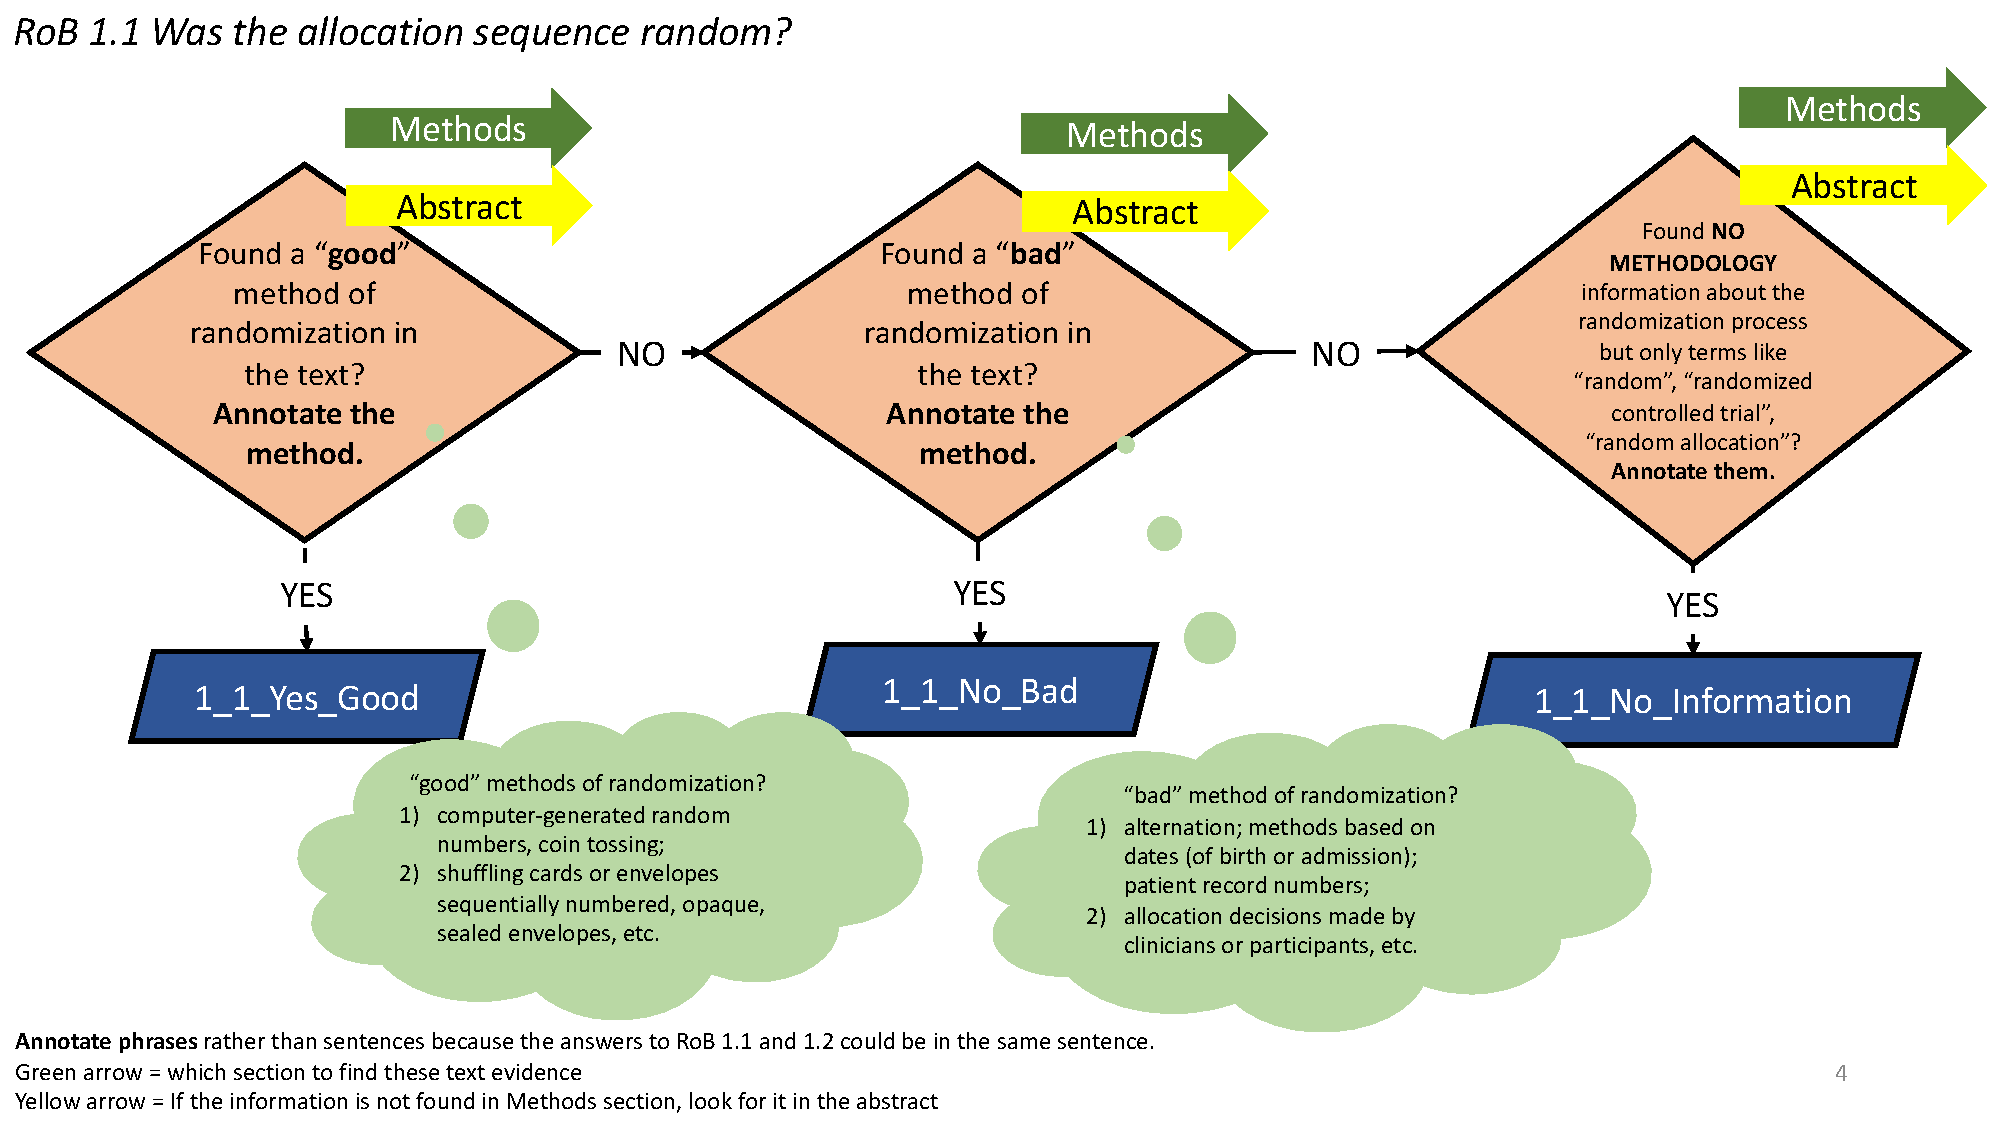
\includegraphics[width=\textwidth]{figures/1_1.pdf}
    \caption{Annotation instructions for the RoB 1.1 signalling question.}
    \label{fig:1_1}
\end{figure}
%
%
%



%Signalling question 1.1 ``Was the allocation sequence random?'' is used to assess the RoB related to the randomization process in a study.
%It aims to determine whether the allocation of participants to different groups or interventions was done in a random manner.
Signalling question 1.1 ``Was the allocation sequence random?'' assesses whether the allocation of participants to different interventions groups was done in a random manner.
If the allocation sequence is generated randomly, this reduces the bias risk, as it ensures that the allocation is not influenced by the researchers' preferences or the participants' characteristics.
Some of the good random allocation methods include simple randomization (coin flipping, random number generator), stratified randomization, blocked randomization, cluster randomization, and adaptive randomization~\cite{sterne2019rob}.
If the allocation sequence was not generated using a proper randomization method, this increases the bias risk in the study.
For e.g., if the allocation sequence was generated using a non-random method, such as alternating assignment or assignment based on participant characteristics, this could introduce bias into the study.
In fact improperly generated allocation sequence or inadequately concealed randomization sequence were associated with larger intervention estimates in RCTs~\cite{bello2017contemporary}.



Follow the Flowchart~\ref{fig:1_1} for annotation instructions of the SQ 1.1: ``Was the allocation sequence random?''.
Following the above explanation, the first diamond in the flowchart instructs the annotators to identify the randomization method for allocation sequence, and if a proper randomization method is found, mark the method description with ``1.1 Yes Good''.
If the text describes a bad or improper method of randomization, mark the text with ``1.1 No Bad''.
This description should be a few words or a phrase and not a complete sentence.
If you did not find any information about the randomization methodology, but if the system finds relating terms like ``random'', ``randomized trial'' or phrases like ``we did random allocation'' are automatically detected, then such phrases will be marked with the label ``1.1 No Information''.
The information about random sequence allocation can be found in the methods section (first priority) or the abstract (second priority).
Notice that for this signalling question, the annotators are required to mark phrases rather than full sentences~\cite{sterne2019rob,saltaji2017randomized}.
%
%
%
\subsection*{Signalling question: 1.2}
%
The signalling question ``Was the allocation sequence concealed until participants were enrolled and assigned to interventions?'' focuses on assessing the bias risk related to allocation concealment in a study.
In RCTs, the allocation sequence determines the order in which participants are assigned to each intervention group.
Adequate concealment of the allocation sequence refers to the process of keeping the sequence hidden from those who are responsible in enrolling and assigning participants to intervention groups.
Proper allocation concealment helps prevent the possibility of selection bias, which can occur if those enrolling participants in the trial have knowledge of the allocation sequence and can manipulate the assignment of participants to intervention groups based on that knowledge.
If the allocation sequence is not adequately concealed until participants are enrolled and assigned to interventions, this can increase the risk of bias and may lead to systematic differences between the intervention groups~\cite{bello2017contemporary}.
For example, if the allocation sequence is known to the investigators or coordinators, they may selectively enroll participants who are more likely to benefit from a particular treatment, or they may assign participants to one treatment group over another based on personal biases.

%
%
%
\begin{figure}[hbt]
    \centering
    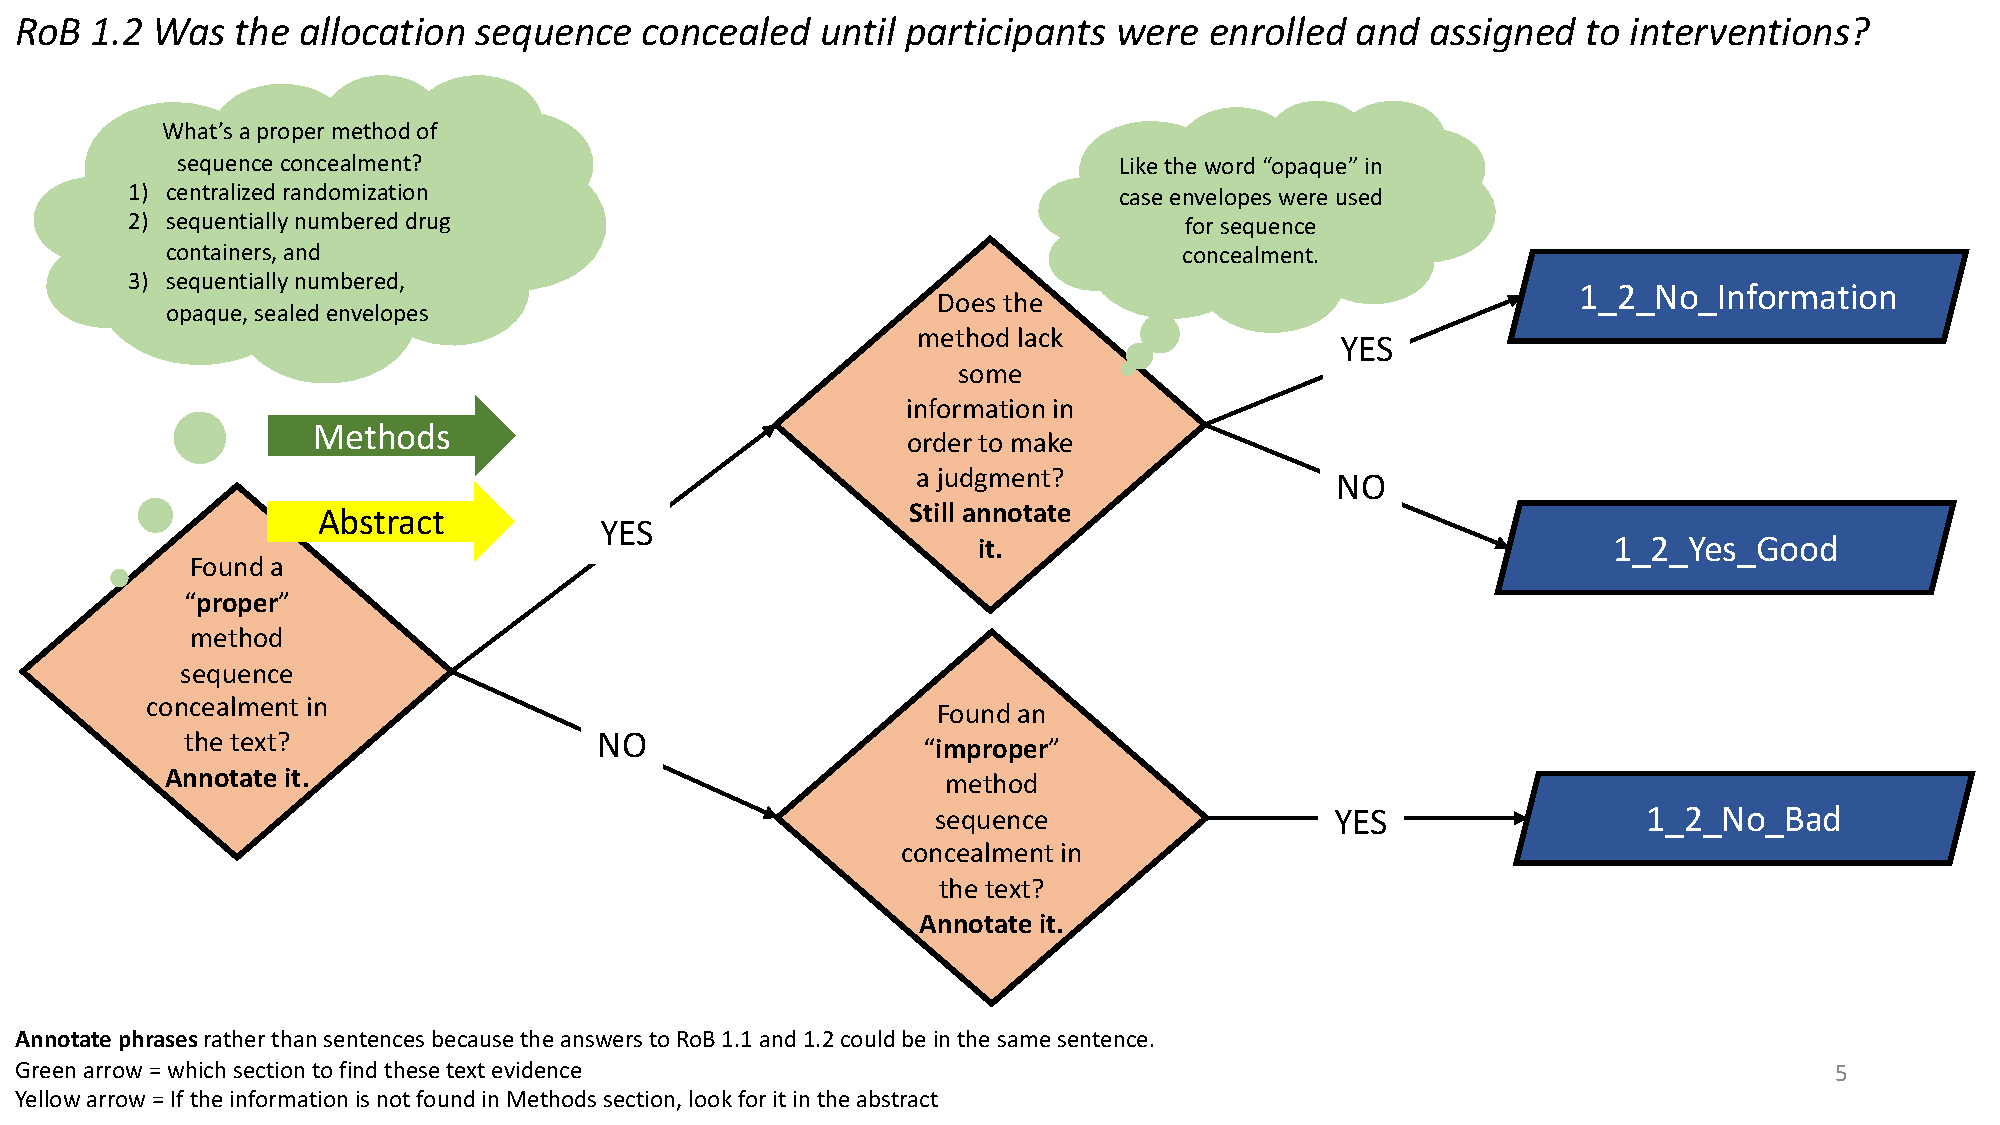
\includegraphics[width=\textwidth]{figures/1_2.pdf}
    \caption{Annotation instructions for the RoB 1.2 signalling question.}
    \label{fig:1_2}
\end{figure}
%
%
%



Follow the Flowchart~\ref{fig:1_2} for annotation instructions of SQ 1.2: ``Was the allocation sequence concealed until participants were enrolled and assigned to interventions?''.
Based on the explanation given earlier, the first diamond in the flowchart guides annotators to identify the method of allocation concealment.
If a proper allocation concealment method is identified but lacks certain details necessary for making a judgment, it should be marked with ``1.2 No Information''.
For instance, if the description mentions the use of sealed envelopes but does not specify whether they were opaque, it would be marked as ``1.2 No Information''.
On the other hand, if enough information is provided to make a judgment, it should be marked with ``1.2 Yes Good''.
Good methods of allocation concealment include central randomization, sealed opaque envelopes, and using online randomization tools that offer to securely generate and conceal the allocation sequence~\cite{sterne2019rob}.
If an improper method of allocation concealment is utilized, then mark the method with ``1.2 No Bad''.
The improper methods of allocation concealment include using an open list, a predictable sequence like alternating using the date of birth or other characteristics, or using the participant's choice.
The primary sources for finding information about allocation concealment are the methods section (first priority, as shown in the Green arrow) and the abstract (second priority, as shown in the yellow arrow)~\cite{sterne2019rob,rahim2021effect}.
%Notice that for this signalling question, too, the annotators are required to mark phrases rather than full sentences.
For this signalling question, annotate a whole sentence if the whole sentence corresponds to answering this question and annotate a phrase if only a part of the sentence does concern answering the question.
For example, annotate the whole sentence ``A computer generated random sequence list was generate with two strata and random block size with sizes of two to eight'' because annotating the whole sentence is necessary to answer the question.
For this next example, annotate only the second part of the sentence, ``A random sequence was generated with a software (stratified for site and with random block sizes), and the allocation was concealed with sealed opaque envelopes.''
%
%
%
\subsection*{Signalling question: 1.3}
%
The signalling question ``Did baseline differences between intervention groups suggest a problem with the randomization process?'' of the RoB 2 tool is related to the potential for bias arising from differences in baseline characteristics between intervention groups that are not related to chance and may suggest a problem with the randomization process.
Even with good randomization, chance imbalances in baseline characteristics can occur leading to an ineffective randomization.
For example, if the treatment group has significantly more female participants, older participants, or participants with more severe disease at baseline compared to the control group, this may suggest that the randomization process was not effective or that there was a problem with the allocation sequence.
This can lead to biased estimates of treatment effects and decrease the internal validity of the study.
If there are significant differences in baseline characteristics between intervention groups that are not related to chance, this may suggest that the randomization process was not effective, and the reliability of the study results may be decreased~\cite{roberts1999baseline}.


%
%
%
\begin{figure}[hbt]
    \centering
    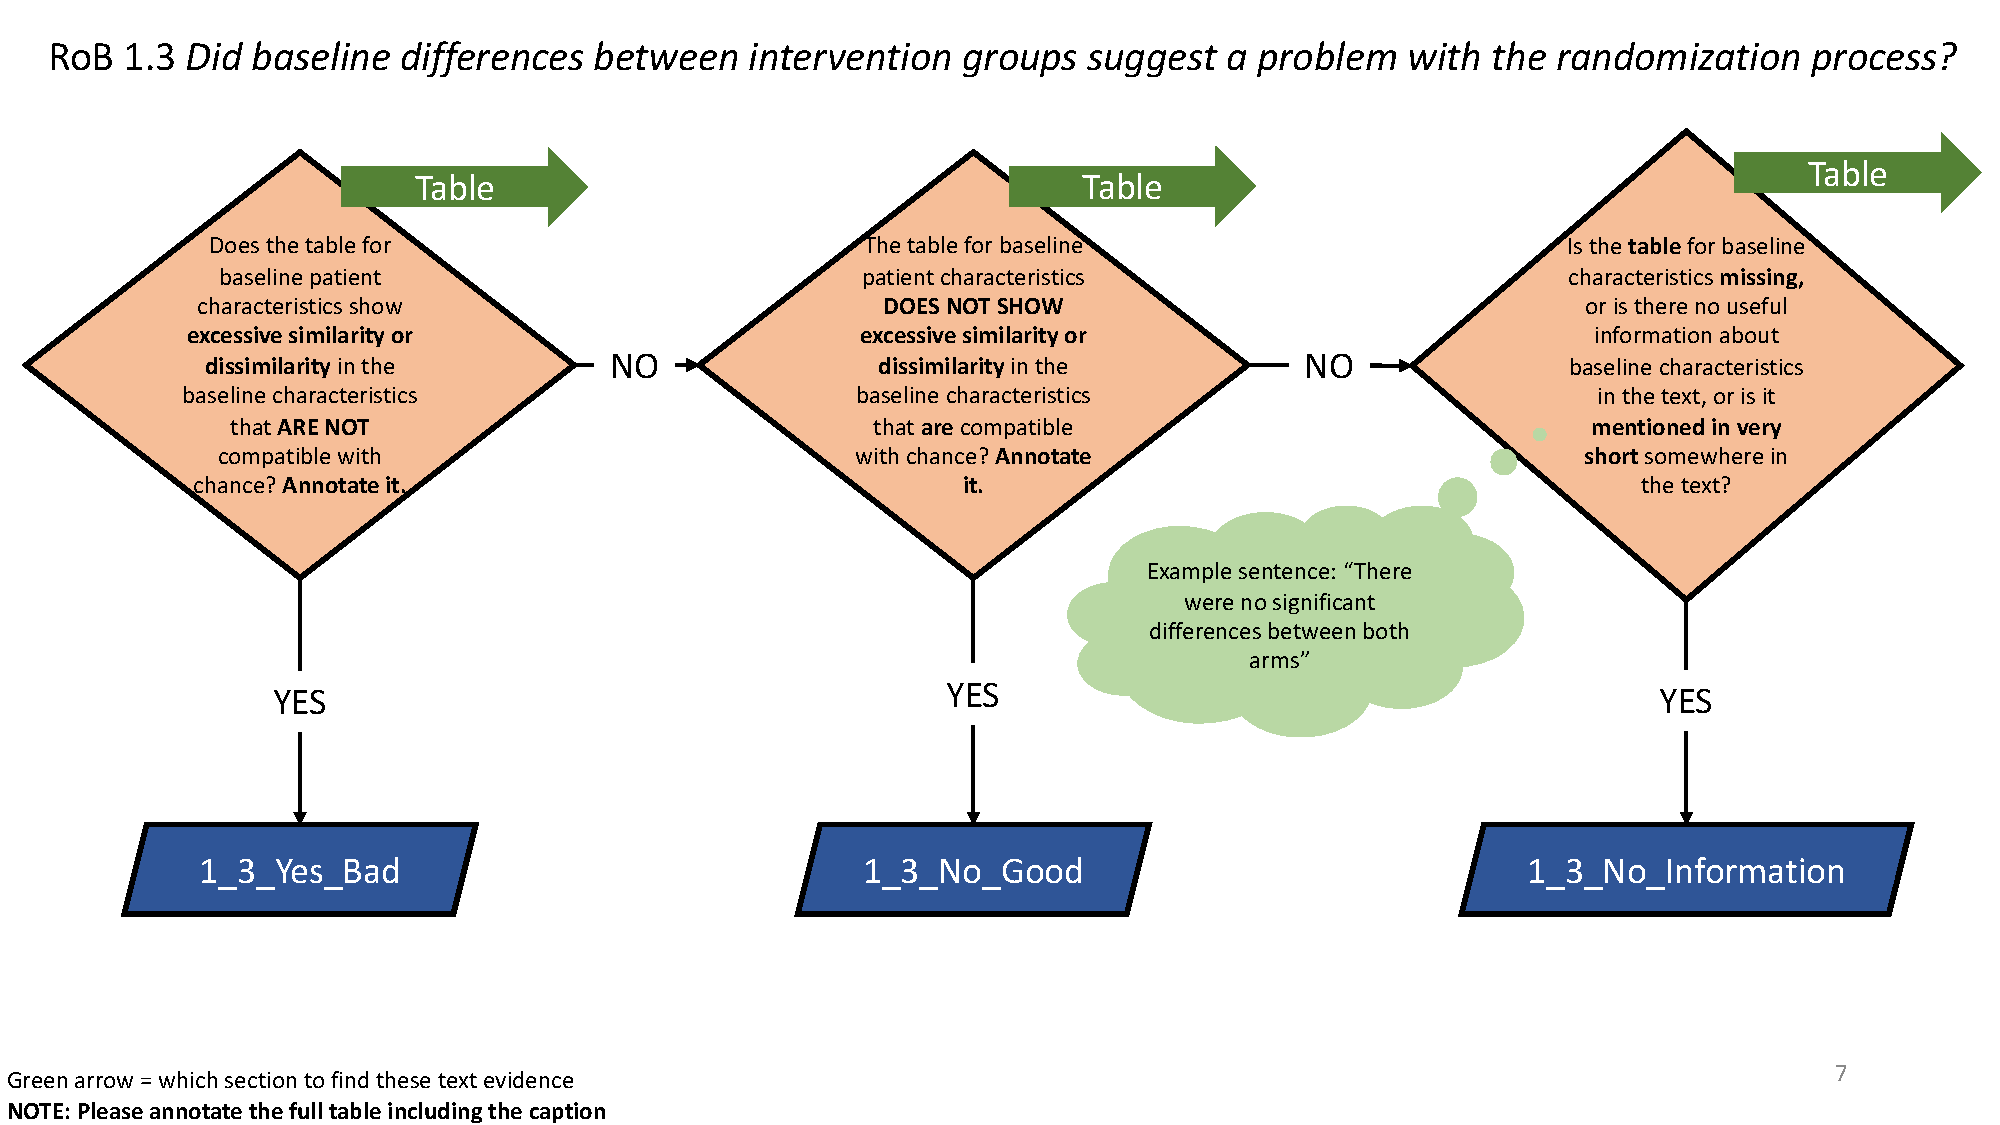
\includegraphics[width=\textwidth]{figures/1_3.pdf}
    \caption{Annotation instructions for the RoB 1.3 signalling question.}
    \label{fig:1_3}
\end{figure}
%
%
%


Follow the Flowchart~\ref{fig:1_3} for annotation instructions of the SQ, ``Did baseline differences between intervention groups suggest a problem with the randomization process?''.
The information to assess this question could be found in the table describing the demographic and clinical baseline characteristics of study participants. 
At this point, the first diamond requests the annotators to mark the full table instead of one or two characteristics, as extracted table text from PDFs lack the inherent structure necessary for training machine learning models.
Therefore, it will be difficult to use the extracted table text to train the machine learning models effectively. 
If the table for baseline patient characteristics shows excessive similarity or dissimilarity in the baseline characteristics that ARE NOT compatible with chance, then mark the full table as well as table caption with the label ``1.3 Yes Bad'' otherwise, mark the full table and the table caption with the label ``1.3 No Good''.
In some cases, this table is missing, but there could be text descriptions that could hint towards baseline differences that could act as confounding factors.
For instance, consider the following sentence, ``Because baseline ODI differences were a potential confounding factor, an adjusted multiple linear and logistic regression analysis was performed for each continuous and categorical outcome measure...''~\citep{cohen2008randomized}.
If you find any such information in the full text, mark it with the label ``1.3 No Information''.
The goal is to capture any relevant information in the full text or table that can help determine if baseline differences between intervention groups indicate a problem with randomization.
%
%
%
%%%%%%%%%%%%%%%%%%%%%%%%%%%%%%%%%%%%%%%%%%%%%%%%%%%%%
\section*{Annotation Guidelines for RoB domain 2}
\label{sec:dom2}
%%%%%%%%%%%%%%%%%%%%%%%%%%%%%%%%%%%%%%%%%%%%%%%%%%%%%
%
The second risk domain in the RoB 2 tool is referred to as ``bias due to deviations from intended interventions''.
In RCTs, it is essential to ensure that participants in a study are assigned to the intended interventions accurately and that the interventions are administered as planned.
However, there can be deviations from the intended interventions when participants do not receive the assigned treatment or when they do not adhere to the prescribed regimen.
This can happen for various reasons, such as non-compliance by participants, crossovers between treatment groups, or missing data due to dropout or loss to follow-up.
In fact, trials that deviated from the intention to treat analysis showed larger intervention effects~\cite{abraha2015deviation}.


NOTE: Before detailing the annotation instructions for signalling questions, we clarify the difference between deviations from intended interventions and dropouts from the trial.
Deviations from intended interventions are any unintentional changes that could have occurred in the treatment under investigation in the trial.
For example, participants may not have complied with the study protocol, or there might have been problems with the delivery of the intervention that could have influenced the study outcomes.
In contrast, dropouts refer to participants who withdrew from the study or were lost to follow-up.
Dropouts can potentially introduce bias into a study if the characteristics of the participants who dropped out are different from those who completed the study.
High dropout rates can also affect the statistical power of the study and its ability to draw valid conclusions.
Although both deviations from the intended intervention and dropout rates can potentially introduce bias into a study, they are not the same thing and should be evaluated separately when assessing the risk of bias in a study~\cite{imel2013meta,cedenilla2023psychosocial}.
%
%
%
\subsection*{Signalling question - 2.1}
\label{subsec:2_1}
%
The SQ 2.1: ``Were participants aware of their assigned intervention during the trial?'' assesses whether the clinical study performed proper blinding or masking of the trial participants.
Blinding or masking of participants is important to minimize the bias risk due to participants' knowledge of their assigned intervention.
When participants are not blinded, they could potentially modify their behaviour, expectations, or reports of outcomes, consciously or unconsciously, based on their knowledge of the assigned intervention, leading to a biased estimate of the treatment effect.
Proper blinding of participants involves concealing the intervention to ensure that the participants do not know which intervention they received~\cite{cedenilla2023psychosocial,swan2003bupropion,o2012rethinking}.
Proper blinding of participants in physiotherapy and rehabilitation domains is challenging due to the nature of the interventions. 
In these domains blinding may not be possible in studies because the treatment and control pairs involve a clear difference in the type or frequency of therapy being delivered, such as exercise interventions, behavioural interventions, educational interventions, and mind-body interventions~\cite{andersson2020effect,buttery2023lung}.
% Some of good blinding strategies for these domain are listed below.
%Proper blinding in rehabilitation trials can be challenging, but several methods can be used to minimize the risk of bias due to the knowledge of the assigned intervention by the study participants and therapists.
%These methods include the use of placebo or sham interventions; for example, in studies of manual therapy, a sham therapy such as light touch or a placebo intervention like ultrasound can be used to blind the participants, and use of standardized interventions, therapist blinding, remote monitoring, and masking techniques.
%Use of placebo or sham interventions: In some rehabilitation trials, a placebo or sham intervention can be used to blind the participants and therapists to the assigned intervention. For example, in studies of manual therapy, a sham therapy such as light touch or a placebo intervention like ultrasound can be used to blind the participants.
%Use of standardized interventions: Standardized interventions can be used to ensure that all participants receive the same intervention regardless of the assigned group. This approach helps reduce the risk of bias and ensures that all participants receive the same level of care.
%Use of therapist blinding: In some rehabilitation trials, therapists can be blinded to the assigned intervention. This approach is particularly useful when the intervention involves physical contact with the participant. For example, in studies of physical therapy, therapists can be trained to provide the same level of care and attention to all participants, regardless of the assigned intervention.
%Use of remote monitoring: In some rehabilitation trials, interventions can be delivered remotely, using telehealth or other technology. This approach can help blind the participants and therapists to the assigned intervention.
%Use of masking techniques: In some rehabilitation trials, masking techniques can be used to conceal the intervention from the participants and therapists. For example, in studies of balance training, participants can be blindfolded to prevent them from seeing the type of training they are receiving.

%
%
%
\begin{figure}[hbt]
    \centering
    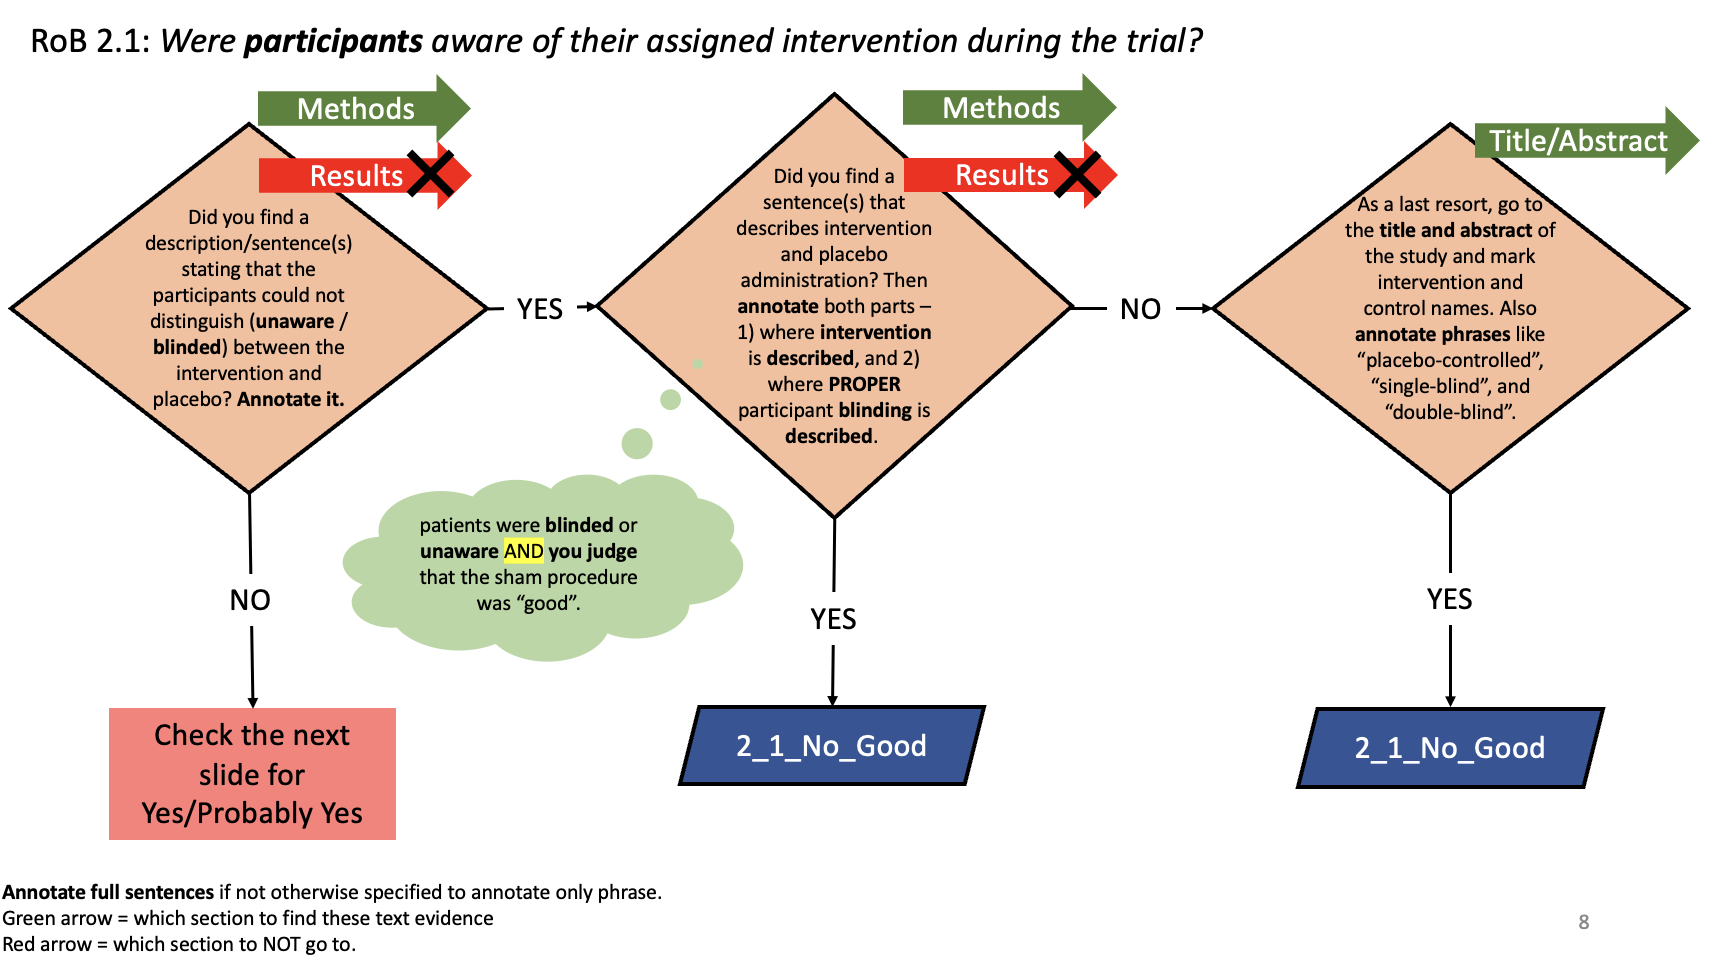
\includegraphics[width=\textwidth]{figures/2_1.png}
    \caption{Annotation instructions for the RoB 2.1 signalling question. (part I)}
    \label{fig:2_1}
\end{figure}
\begin{figure}[hbt]
    \centering
    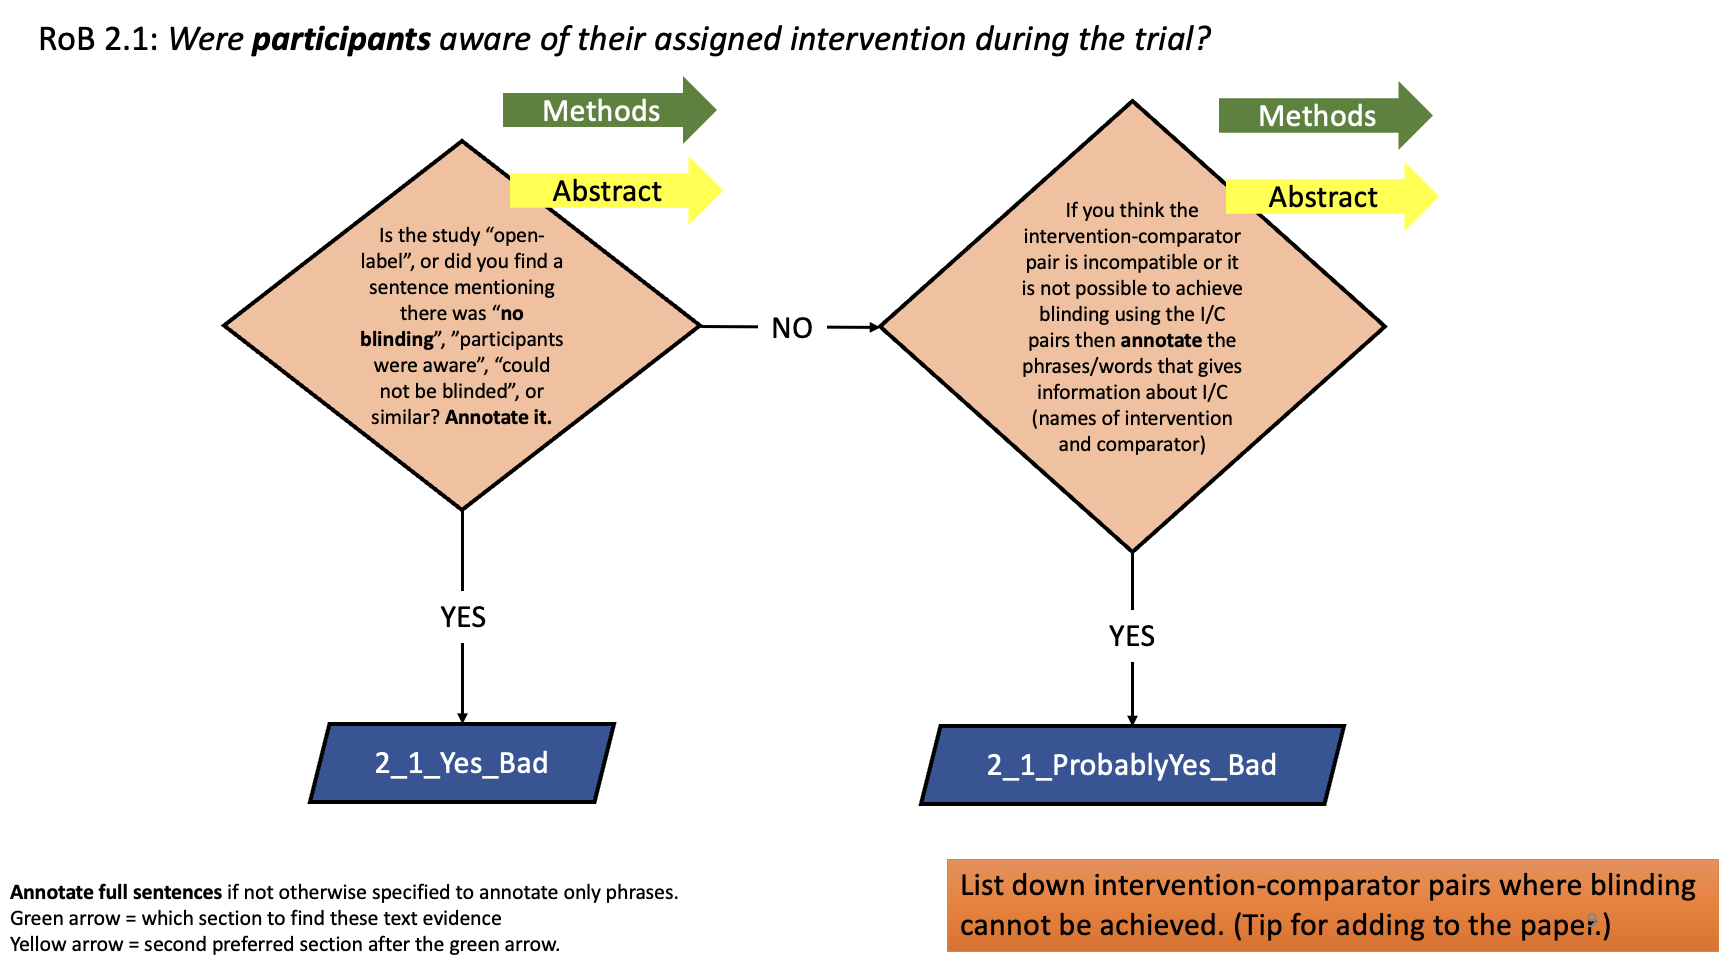
\includegraphics[width=\textwidth]{figures/2_1_1.png}
    \caption{Annotation instructions for the RoB 2.1 signalling question. (part II)}
    \label{fig:2_1_1}
\end{figure}
%
%
%

Follow the Flowcharts~\ref{fig:2_1} and~\ref{fig:2_1_1} for annotation instructions of the SQ 2.1: ``Were participants aware of their assigned intervention during the trial?''.
Following the above explanation, the first diamond in the flowchart asks the annotators to find text descriptions stating that the participants could not distinguish (unaware/blinded) between the assigned interventions (the main intervention and the control intervention).
If such description is found, then annotate it and follow the connector line towards the decision ``yes'', find the sentences that describe intervention and placebo administration and annotate both the descriptions – the first part where intervention administration is described, and the second part where proper participant blinding via a placebo is described.
Annotate these parts with the label ``2.1 No Good''.
Both these administration descriptions can be found either in adjacent sentences or far apart in the same or different paragraphs within the same section.
Annotators are likely to find this information in the methods section and not in the Results section. 
If text parts describing the intervention and placebo administration are not found, but there are phrases in the title or abstract indicating that the study is ``placebo-controlled'', ``single-blind'', ``double-blind'', then mark these phrases with the label ``2.1 No Good''.


Going back to the first diamond, if the annotators did not find any information stating that the participants were unaware of the assigned intervention, they are asked to go to part II of the placard~\ref{fig:2_1_1}.
If the annotators find that the study is ``open-label'', or found the sentence(s) mentioning that there was no blinding, or participants were aware, or could not be blinded, or something along the lines of the sentences mentioned below, then annotate such sentences with the label ``2.1 Yes Bad''.
For example, 1) ``Blinding of trial participants and the trial coordinator was not possible due to the nature of the interventions,...'', and 2) ``...we wanted to evaluate the commonly used methods that often involve parents’ actions, and blinding of parents to participants, care providers, or assessors was not possible due to the nature of the intervention.''~\cite{buttery2023lung,andersson2020effect}.
If the information about the study being ``open-label'' or participants being aware is not found, but the annotator thinks that for the intervention-comparator (IC) pair, it is not possible to achieve blinding using the IC pairs then annotate the phrases/words that give information about IC (names of intervention and comparator) with the label ``2.1 Probably Yes Bad''.
Blinding information can be found either in the methods section or the abstract.
% List down intervention-comparator pairs where blinding cannot be achieved.
%
%
%
\subsection*{Signalling question - 2.2}
\label{subsec:2_2}
%
While the previous signalling question assessed participant blinding, this question, ``Were the carers and people delivering the interventions aware of the participants' assigned intervention during the trial?'' evaluates whether the carers and individuals delivering the interventions were aware of the participants' assigned interventions during the trial.
%Blinding or masking of carers and intervention providers is important to minimize the risk of bias that can arise if they have knowledge of the participants' assigned interventions.
If carers and treatment administrators are not blinded, their awareness of the assigned interventions may influence their behaviour, interactions with participants, and delivery of the interventions potentially introducing bias and affect the study outcomes~\cite{hrobjartsson2011blinding}.



%
%
%
\begin{figure}[hbt]
    \centering
    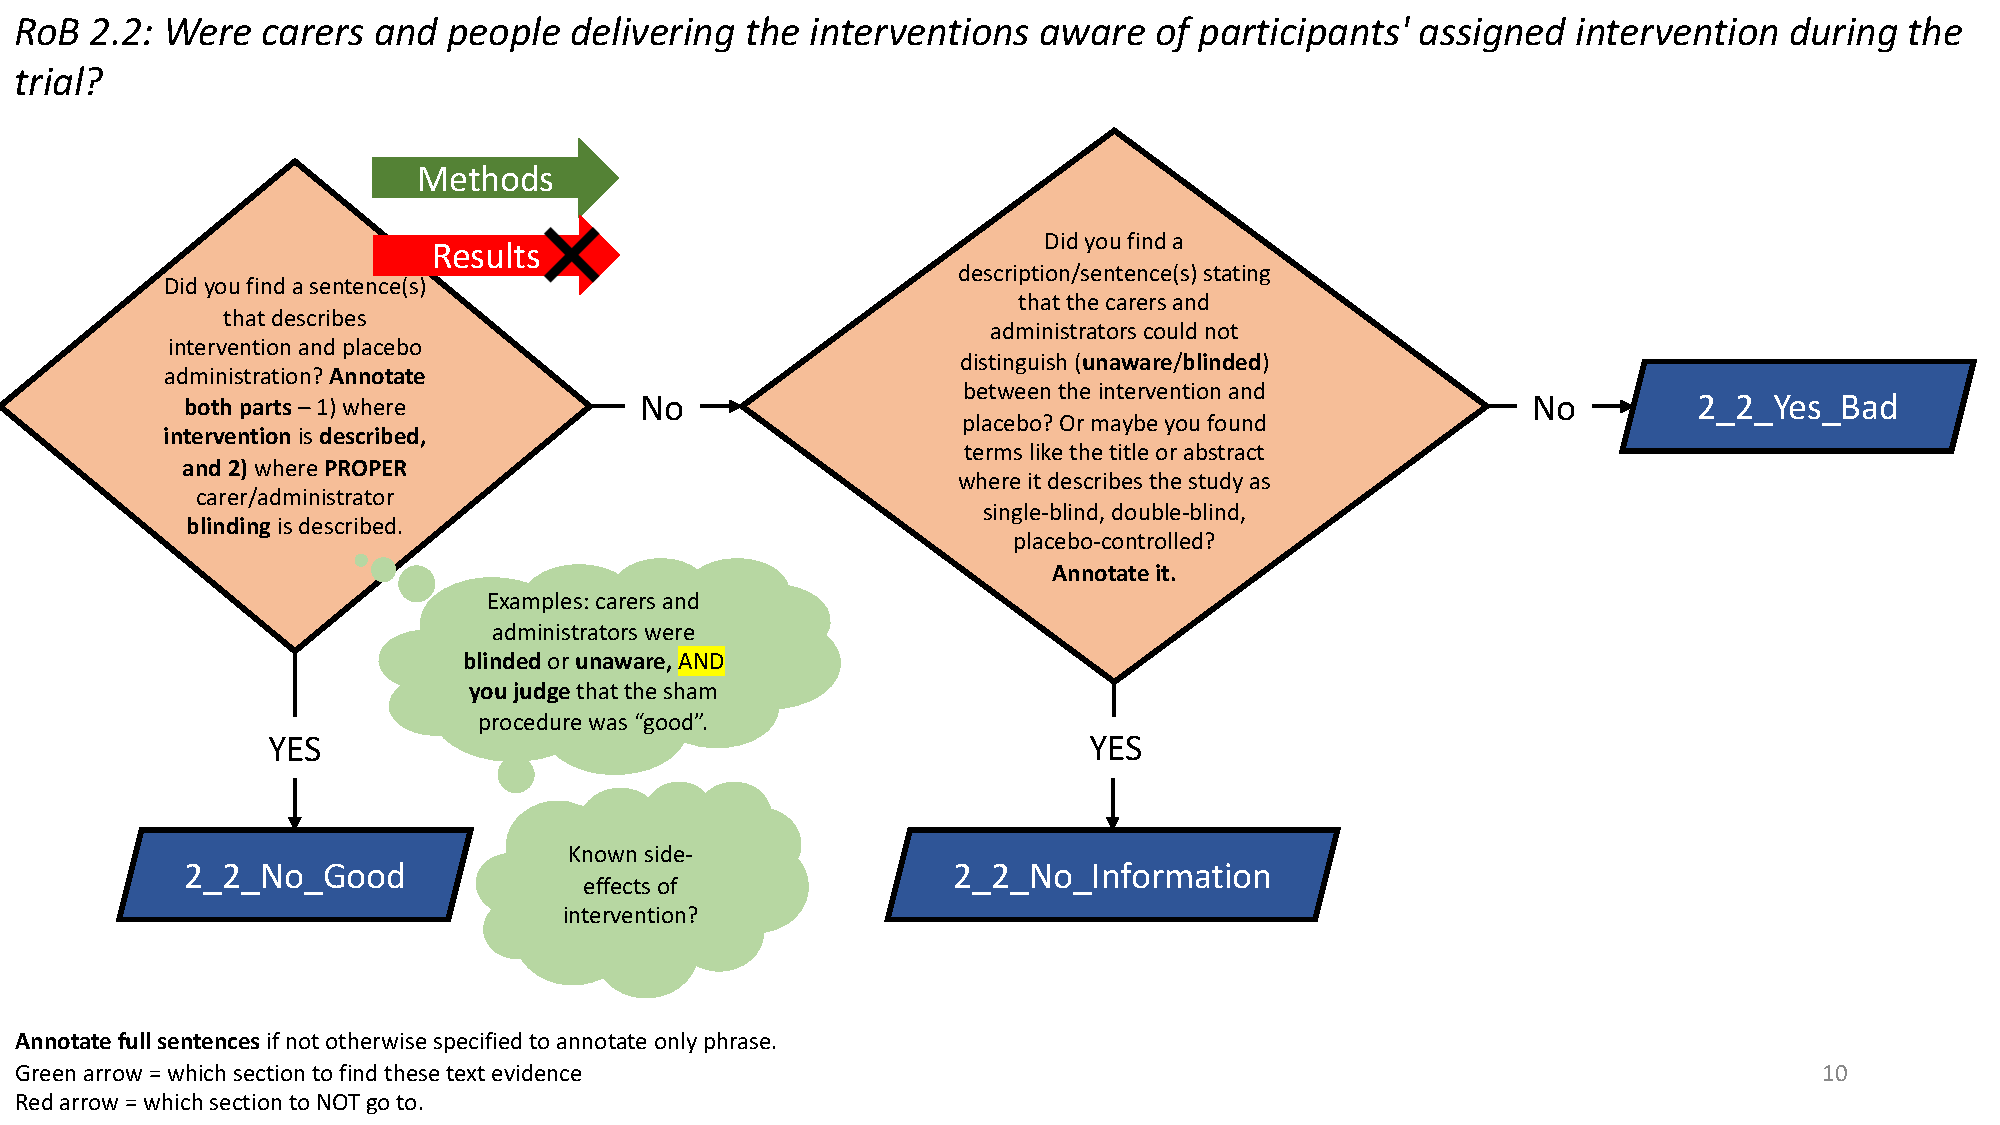
\includegraphics[width=\textwidth]{figures/2_2.pdf}
    \caption{Annotation instructions for the RoB 2.2 signalling question.}
    \label{fig:2_2}
\end{figure}
%
%
%


Follow the Flowcharts~\ref{fig:2_2} for annotation instructions of the signalling question, ``Were the carers and people delivering the interventions aware of the participants' assigned intervention during the trial?''.
Following the above explanation, the first diamond instructs the annotators to find any sentences stating or clearly implying if the carers and administrators could not distinguish between intervention and placebo.
If no such sentences were found, the label ``2.2 No Information'' will be assumed for this question.
If such sentences are found, then annotate them and follow the connector line towards the decision ``yes'', then find the sentences that describe intervention and placebo administration and annotate both the descriptions – the first part where intervention administration is described, and the second part where proper participant blinding via a placebo is described.
Annotate all these parts with the label ``2.1 No Good''.
For example, ``This RCT used a 5-week, double-blind, parallel groups design'', ``Treatment was administered by an RA who was blinded to assessment results and study hypotheses''\cite{chiaravalloti2020efficacy}.
If no proper carer blinding was described or if it was explicitly mentioned that carer blinding was not possible, then the sentences identified using the first diamond should be marked with the label ``2.2 Yes Bad''.
For example, ``...we wanted to evaluate the commonly used methods that often involve parents’ actions, and blinding of parents to participants, care providers, or assessors was not possible due to the nature of the intervention''~\cite{andersson2020effect}.



%
%
%
\subsection*{Signalling question - 2.3}
\label{subsec:2_3}
%
This signalling question 2.3, ``Were there deviations from the intended intervention that arose because of the trial context?'' aims to assess the risk of bias associated with deviations from the intended intervention in a study.
It seeks to determine whether any deviations occurred during the trial due to factors related to the trial context.
The intended intervention refers to the specific treatment or intervention that is planned to be delivered to participants.
Deviations from the intended intervention can occur for various reasons, such as practical challenges, implementation issues, or unforeseen circumstances within the trial context~\cite{paterson2019feasibility}.
This question focuses on assessing whether these deviations from the intended intervention were due to factors directly related to the trial rather than factors outside the trial.
It helps evaluate the extent to which the trial protocol was followed and whether the trial results could have been influenced by these deviations.

%
%
%
\begin{figure}[hbt]
    \centering
    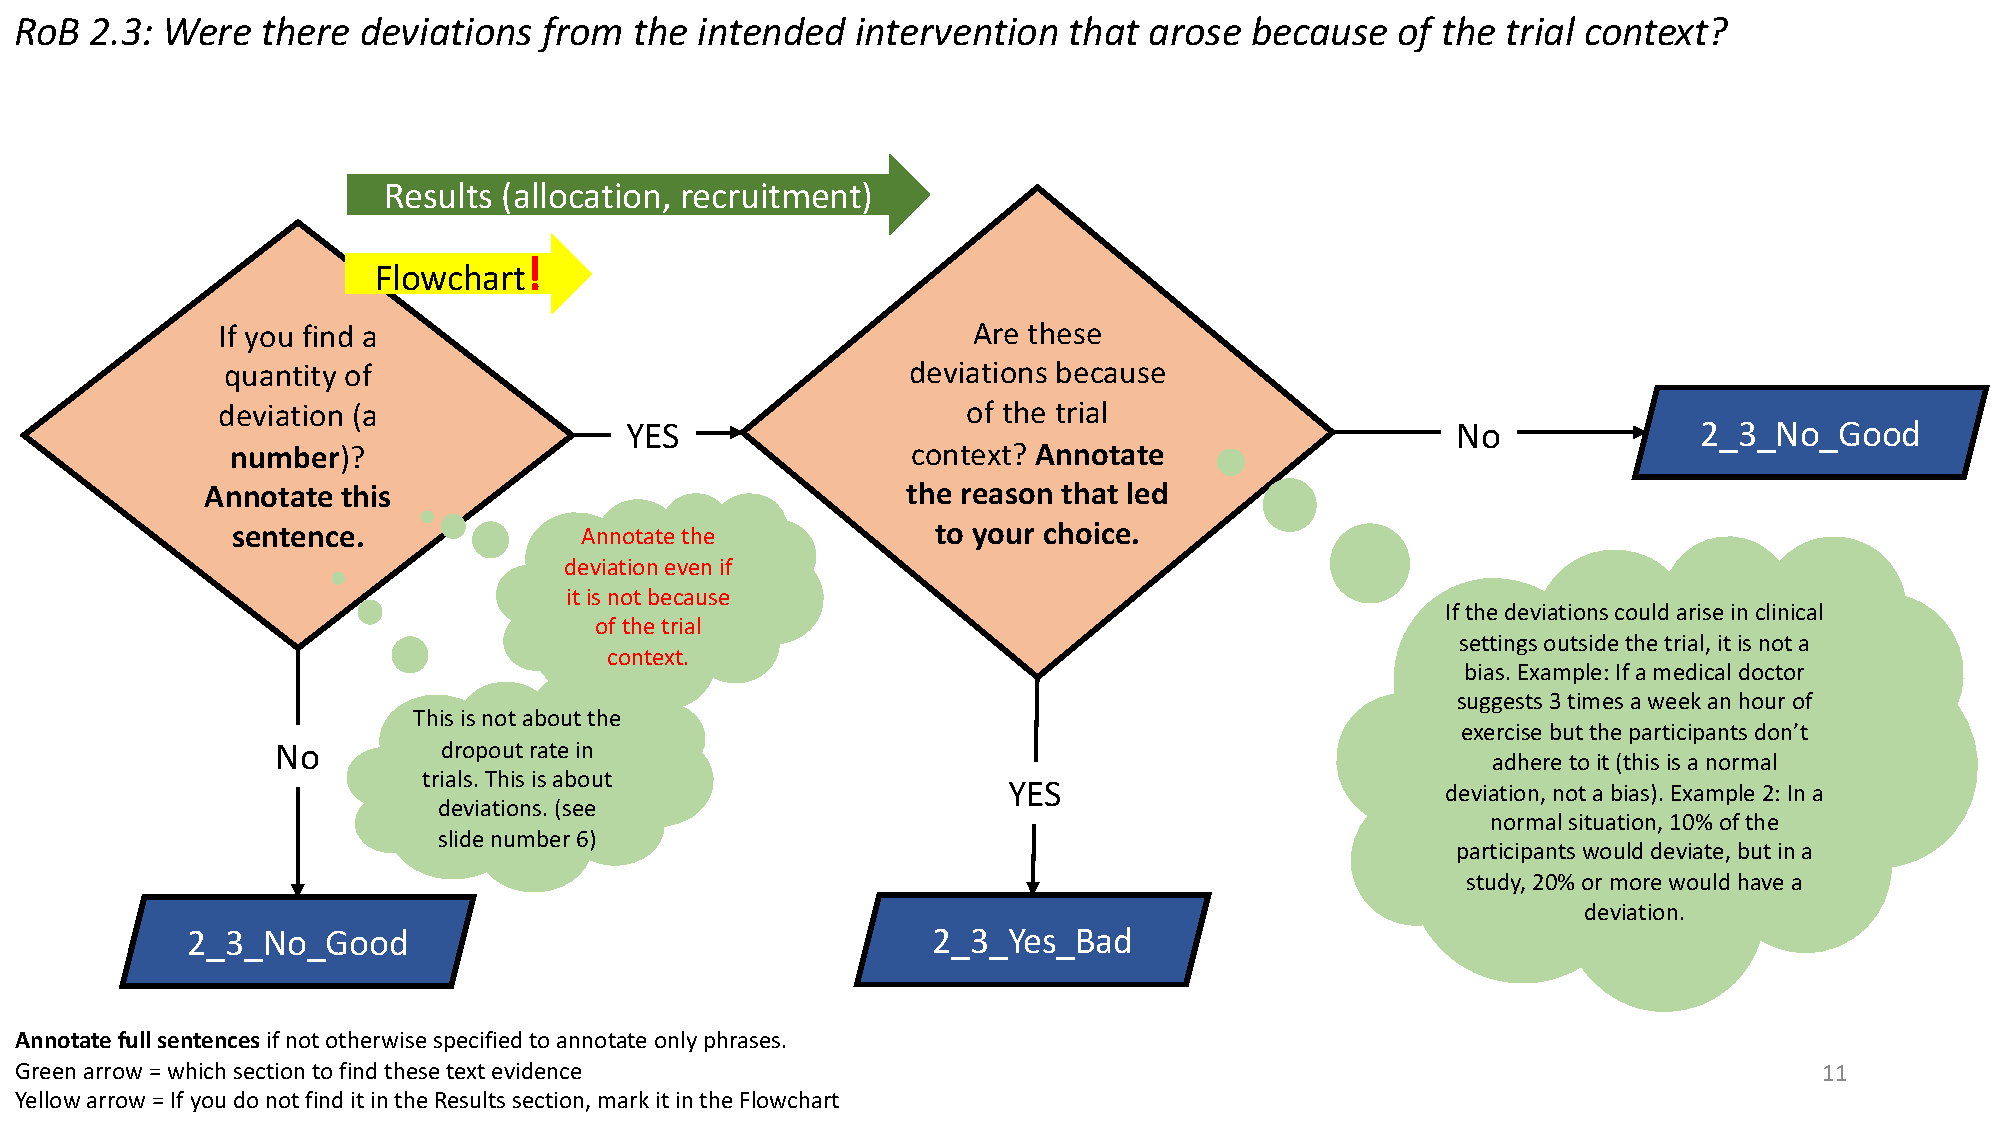
\includegraphics[width=\textwidth]{figures/2_3.pdf}
    \caption{Annotation instructions for the RoB 2.3 signalling question.}
    \label{fig:2_3}
\end{figure}
%
%
%

Follow the Flowchart~\ref{fig:2_3} for annotation instructions of the signalling question, ``Were there deviations from the intended intervention that arose because of the trial context?''.
In the flowchart, the first diamond prompts annotators to search for information regarding the number of deviations from the intended intervention.
It clarifies that these deviations are not related to the dropout rate in the trial.
If no percentage or absolute number of deviations is identified in the text, no annotation is necessary, and the document will be automatically marked as ``2.3 No Information'' for this signalling question, following the  ``No'' arrow.
If the percentage of deviations is identified, annotators should annotate the full sentence where this information is found.
%For example, during the course of a trial, a certain number of patients could deviate from their assigned intervention or failed to adhere to the prescribed treatment due to various reasons such as lack of improvement, side effects, or personal preference.
They should then proceed to the next diamond in the flowchart, following the ``yes'' flow, and assess whether these deviations occurred due to the trial context.
If the deviations are determined to be due to the trial context, the annotated sentence(s) should be marked as ``2.3 Yes Bad''.
If the deviations are not attributed to the trial context, they should be marked as ``2.3 No Good''.
For example, ``Two patients in the control group receiving physiotherapy (usual care) erroneously attended the PT-led education and exercise programme after...''~\cite{osteraas2019implementing}. % Anjani: requires fact-checking if this is 2.3 Yes Bad or No Good
Additionally, if annotators identify the reasons for their choices of ``no good'' or ``yes bad'', they should mark the sentences explaining their rationale.
It is important to note that a second annotation may be required if there are supporting sentences for the reason behind the choice.
This second annotation allows for capturing additional information.
This information can be found in the text of the Results section, specifically within the allocation or recruitment paragraphs (indicated by the green-coded arrow on the diamonds).
Only if the information is not found in the Results section, should the annotators check the flowcharts or their captions for any relevant details.
The judgment regarding the trial context and deviations can be subjective, and it is left to the reviewers' discretion once they have access to the deviation information.
However, at least the annotators will have the annotated information about the percentage/number of deviations which could be used to train the machine learning models.
Ultimately, the review of deviations and trial context is subjective, but the annotated information can be used to train machine learning models.
%
%
%
\subsection*{Signalling question - 2.4 }
\label{subsec:2_4}
%
%
%
\begin{figure}[hbt]
    \centering
    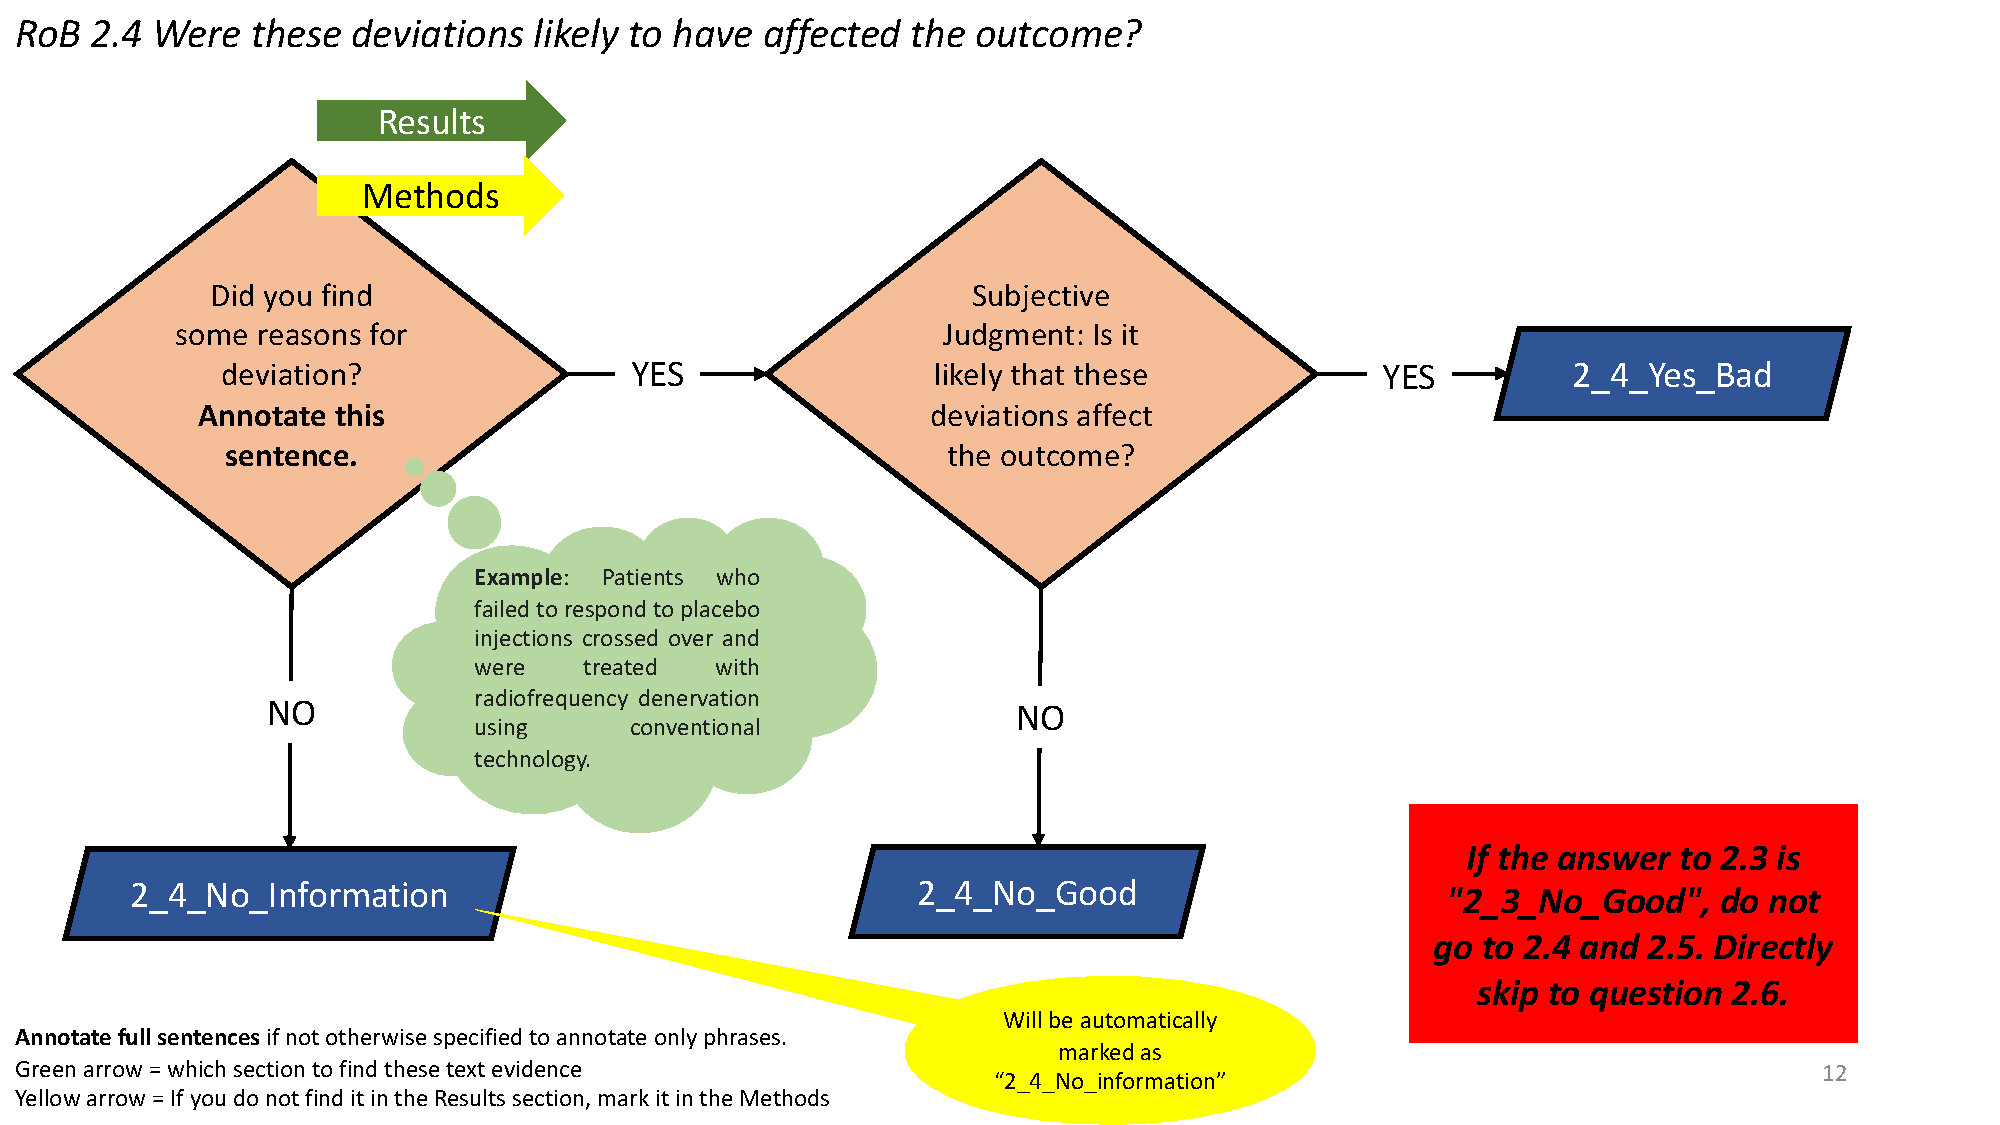
\includegraphics[width=\textwidth]{figures/2_4.pdf}
    \caption{Annotation instructions for the RoB 2.4 signalling question.}
    \label{fig:2_4}
\end{figure}
%
%
%
In RCTs, deviations from the planned study protocol may occur for various reasons, such as the participant not following the intervention as intended, the trial site not adhering to the study procedures, external constraints or trial discontinuation.
These deviations are known as ``protocol deviations''~\cite{folayan2019challenges,merli2020immediate}.
The question ``Were these deviations likely to have affected the outcome?'' refers to whether the protocol deviations had the potential to influence the study outcomes.
If the identified deviations (identified using the previous questions) are determined to have a substantial likelihood of affecting the study outcomes, it suggests a higher risk of bias~\cite{dodd2012nonadherence}. 
Conversely, if the deviations are deemed unlikely to have influenced the outcomes significantly, it indicates a lower risk of bias.
Assessing the impact of deviations on the outcomes requires a thorough understanding of the study design, interventions, and potential sources of bias.
It may involve considering factors such as the timing, frequency, and magnitude of the deviations, as well as their relevance to the study objectives and population under investigation.
%Ultimately, the judgment regarding the influence of deviations on the outcomes is subjective and requires careful interpretation of the available information and expertise in the specific research domain.
%The aim of this question is to assess the RoB due to the protocol deviations, which may have introduced systematic error or affected the internal validity of the study.
%If the deviations were unlikely to have affected the study outcome, then this question would be answered with "No."
%However, if the deviations were likely to have affected the study outcome, then this question would be answered with "Yes," indicating that the study is at high risk of bias.
%If it is unclear whether the deviations affected the outcome, the answer would be "Some concerns."



For annotation instructions for this signalling question, ``Were these deviations likely to have affected the outcome?'' follow the Flowchart~\ref{fig:2_4}.
Before proceeding with the annotation, ensure that the previous question was not marked as ``2.3 No Good'' (in this case either no deviations were identified or they were not significant).
If it was, no annotation is required for this question.
Otherwise, follow the instructions below.
The first diamond prompts the annotators to identify the reasons for deviations and, if found, they mark it, then follow the connector path of ``yes'' and judge whether these deviations could affect the outcome.
If the annotated reasons could cause some deviation, then mark them as ``2.4 Yes Bad'' and ``2.4 No Good'' otherwise.
%For example, ``Due to logistical constraints, three participants in the intervention group did not receive the prescribed medication as per the study protocol.'' could cause high risk of bias.
%Anjani: (TODO) Could this really cause high risk of bias or is it low risk since only three participants are affected? %Anjani: Give examples for low risk of bias deviations and high risk of bias deviations.
Annotate full sentences for this question.
The reasons could be found either in the Results section (main priority) or the Methods section (second priority).
If the reasons for deviations are not found, then the question is assumed to have ``No Information''.
%To annotate the information pertaining to the previous question, the annotators identify the percentage of deviation (a number) and annotate them, while for this question, the annotators are prompted to look for the reasons for these deviations and annotate them.
%The reasons could be found in either the Results section or in the Method section if not in the Results section.
%For example, this sentence from Osteras 2019 Patient Reporting Quality of Care 6months IAA Hilfiker Sattelmayer with Protocol.pdf ... "['Two patients in the control group receiving physiotherapy (usual care) erroneously attended the PT-led education and exercise programme after their PT had attended the workshop.']" says that some participants went to different therapy "by error/mistake" which is a reason for the deviation, but as it was a small deviation, the annotator marked it as "no good".
%
%
%
\subsection*{Signalling question - 2.5 }
%
%
%
\begin{figure}[hbt]
    \centering
    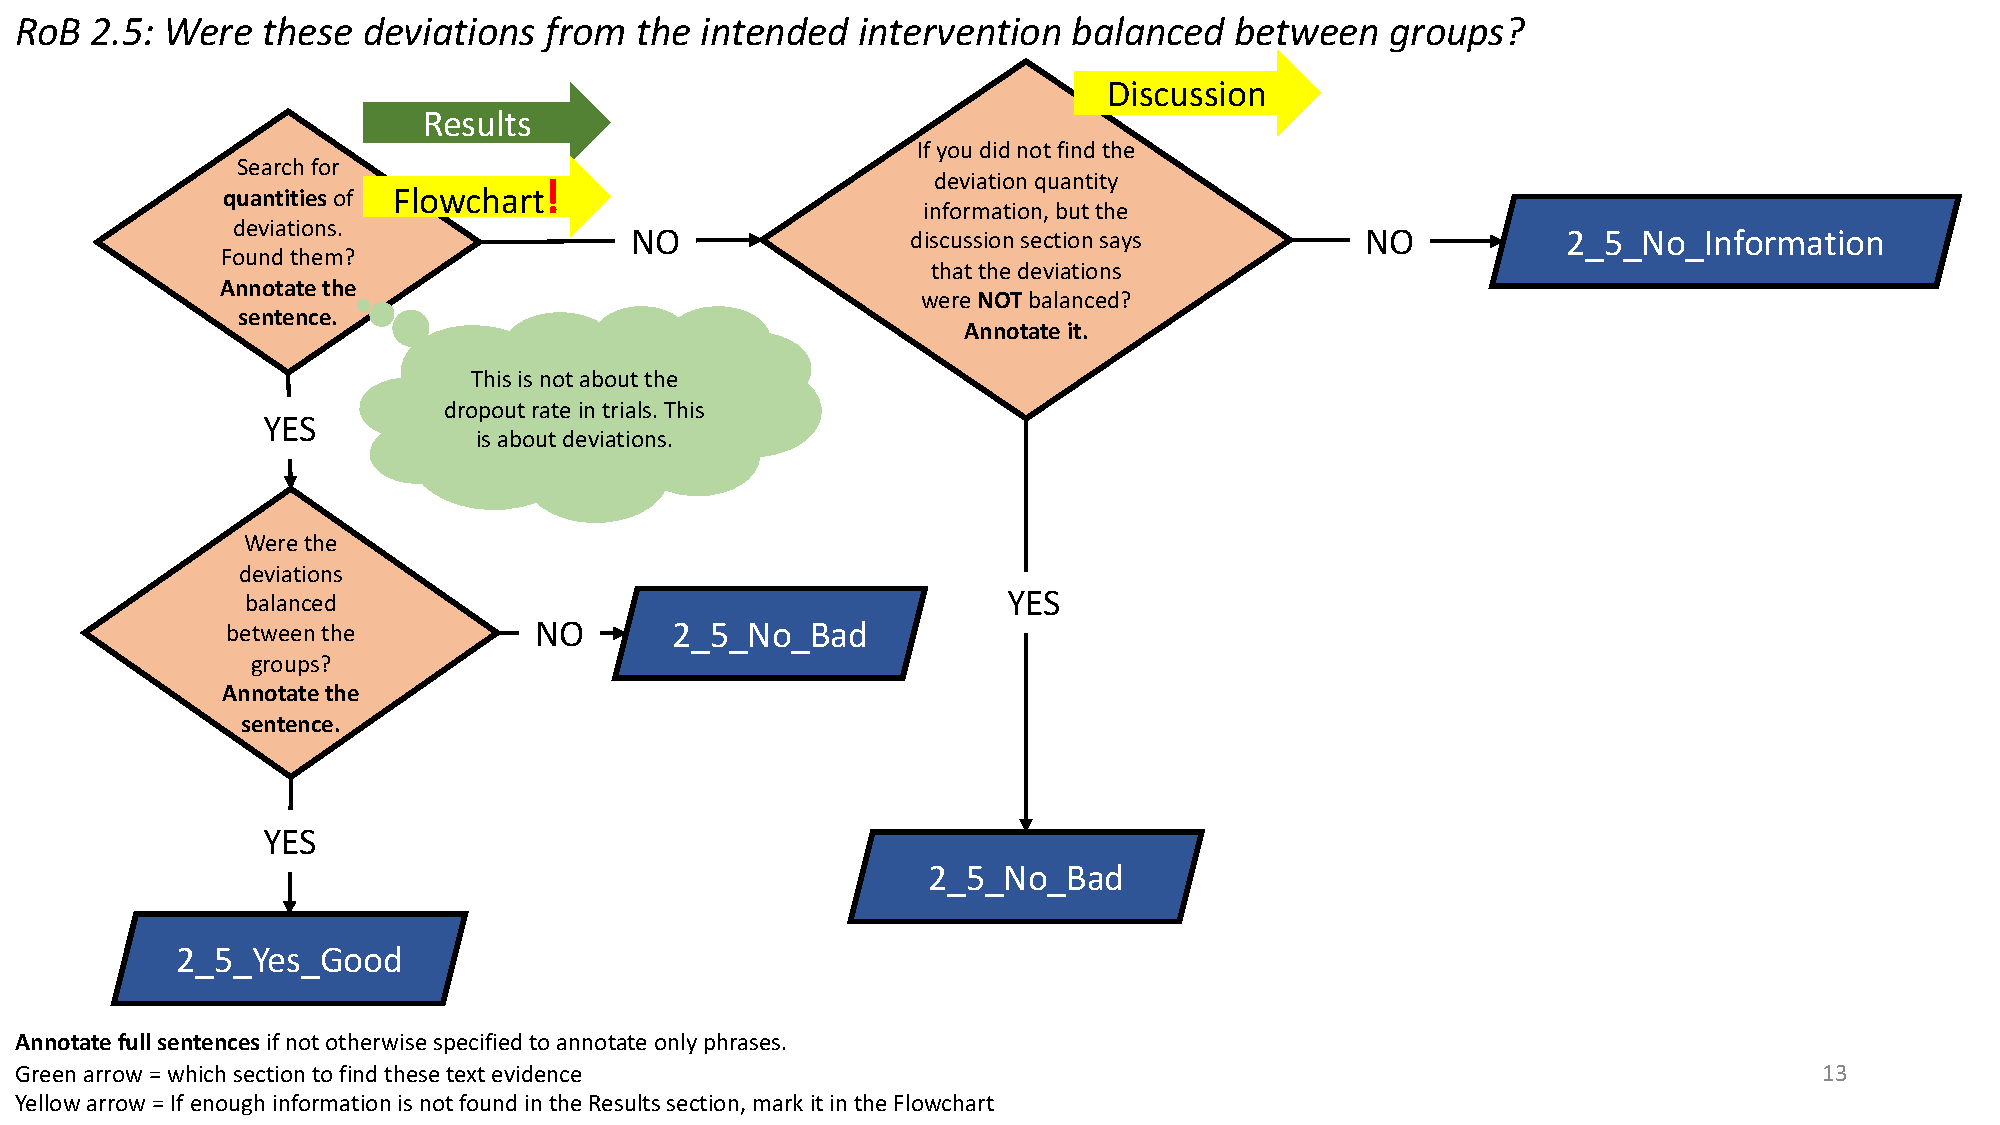
\includegraphics[width=\textwidth]{figures/2_5.pdf}
    \caption{Annotation instructions for the RoB 2.5 signalling question.}
    \label{fig:2_5}
\end{figure}
%
%
%
This signalling question 2.5, ``Were these deviations from the intended intervention balanced between groups?'' aims to assess whether any deviations from the intended intervention were similar in frequency and severity across the different study groups (i.e., intervention group and control group) or whether one group had a greater number or severity of deviations than the other.
Balanced deviations between groups are important for maintaining the internal validity of the study.
If one group had a higher number or severity of deviations from the intended intervention than the other, it could potentially introduce bias and confound the results of the study.
Therefore, it is important to assess whether deviations from the intended intervention were balanced between the groups when evaluating the risk of bias in an RCT~\cite{rozenfeld2006effect}.



For annotation instructions for this signalling question, ``Were these deviations from the intended intervention balanced between groups?'' follow the Flowchart~\ref{fig:2_5}.
The first diamond in the flowchart instructs annotators to search for quantities or numbers indicating deviations from the intended intervention.
It is important to distinguish between deviations and dropout rates (refer to the note in subsection~\ref{sec:dom2} for clarification).
Focus on identifying any numerical information that demonstrates deviations from the intended intervention.
If the deviations are balanced between the groups, mark them as ``2.5 Yes Good''.
If they are not balanced, mark them as ``2.5 No Bad''.
In cases where no quantification of deviations is found, but the Discussion section mentions that the deviations were not balanced, mark that text in the discussion as ``2.5 No Bad''.
For example, ``In the standard care group, the use of corticosteroids in 14 patients (9.4\%) was considered a protocol deviation, and the...'' should be marked as ``2.5 No Bad''~\cite{tomazini2020effect}.
In contrast, ``There were only few missing data because of premature withdrawal, and they were balanced in numbers across the 2 groups with similar reasons for missing data.'' should be marked as ``2.5 Yes Good''~\cite{prodeus2016fermented}.
If no text is marked, the document will receive a ``No Information'' label for this signalling question.
Ensure that the annotation reflects the presence or absence of balanced deviations and consider both quantitative information and relevant discussion text to make an accurate annotation.
%
%
%
\subsection*{Signalling question - 2.6 }
\label{subsec:2_6}
%
The signalling question ``Was an appropriate analysis used to estimate the effect of assignment to intervention?'' evaluates whether the analysis performed to estimate the effect of assigning participants to interventions in the study was reliable and valid.
Participants' assignment to intervention is key to unbiasedly determining the causal relationship between the intervention and outcome.
To ensure the validity and reliability of the study results, it is essential to use appropriate statistical methods and analytical techniques when estimating the effect of assignment to interventions.
So this question assesses the risk of bias associated with the analysis methodology applied. 
An appropriate analysis involves using valid statistical tests, appropriate control for confounding variables, and properly considering potential sources of bias or confounding~\cite{gupta2011intention}. 
%This signalling question evaluates whether the analysis performed in the study was appropriate and reliable in estimating the intervention's effect.
%The aim is to assess the risk of bias associated with the analysis methodology.
%An appropriate analysis involves using valid statistical tests, appropriate control for confounding variables, and proper consideration of potential sources of bias or confounding. 
%The goal is to minimize the risk of drawing incorrect conclusions or overestimating the effect of the intervention.
%By assessing the adequacy of the analysis, this signalling question helps evaluate the internal validity of the study and the confidence in the reported effect of the intervention.


%
%
%
\begin{figure}[hbt]
    \centering
    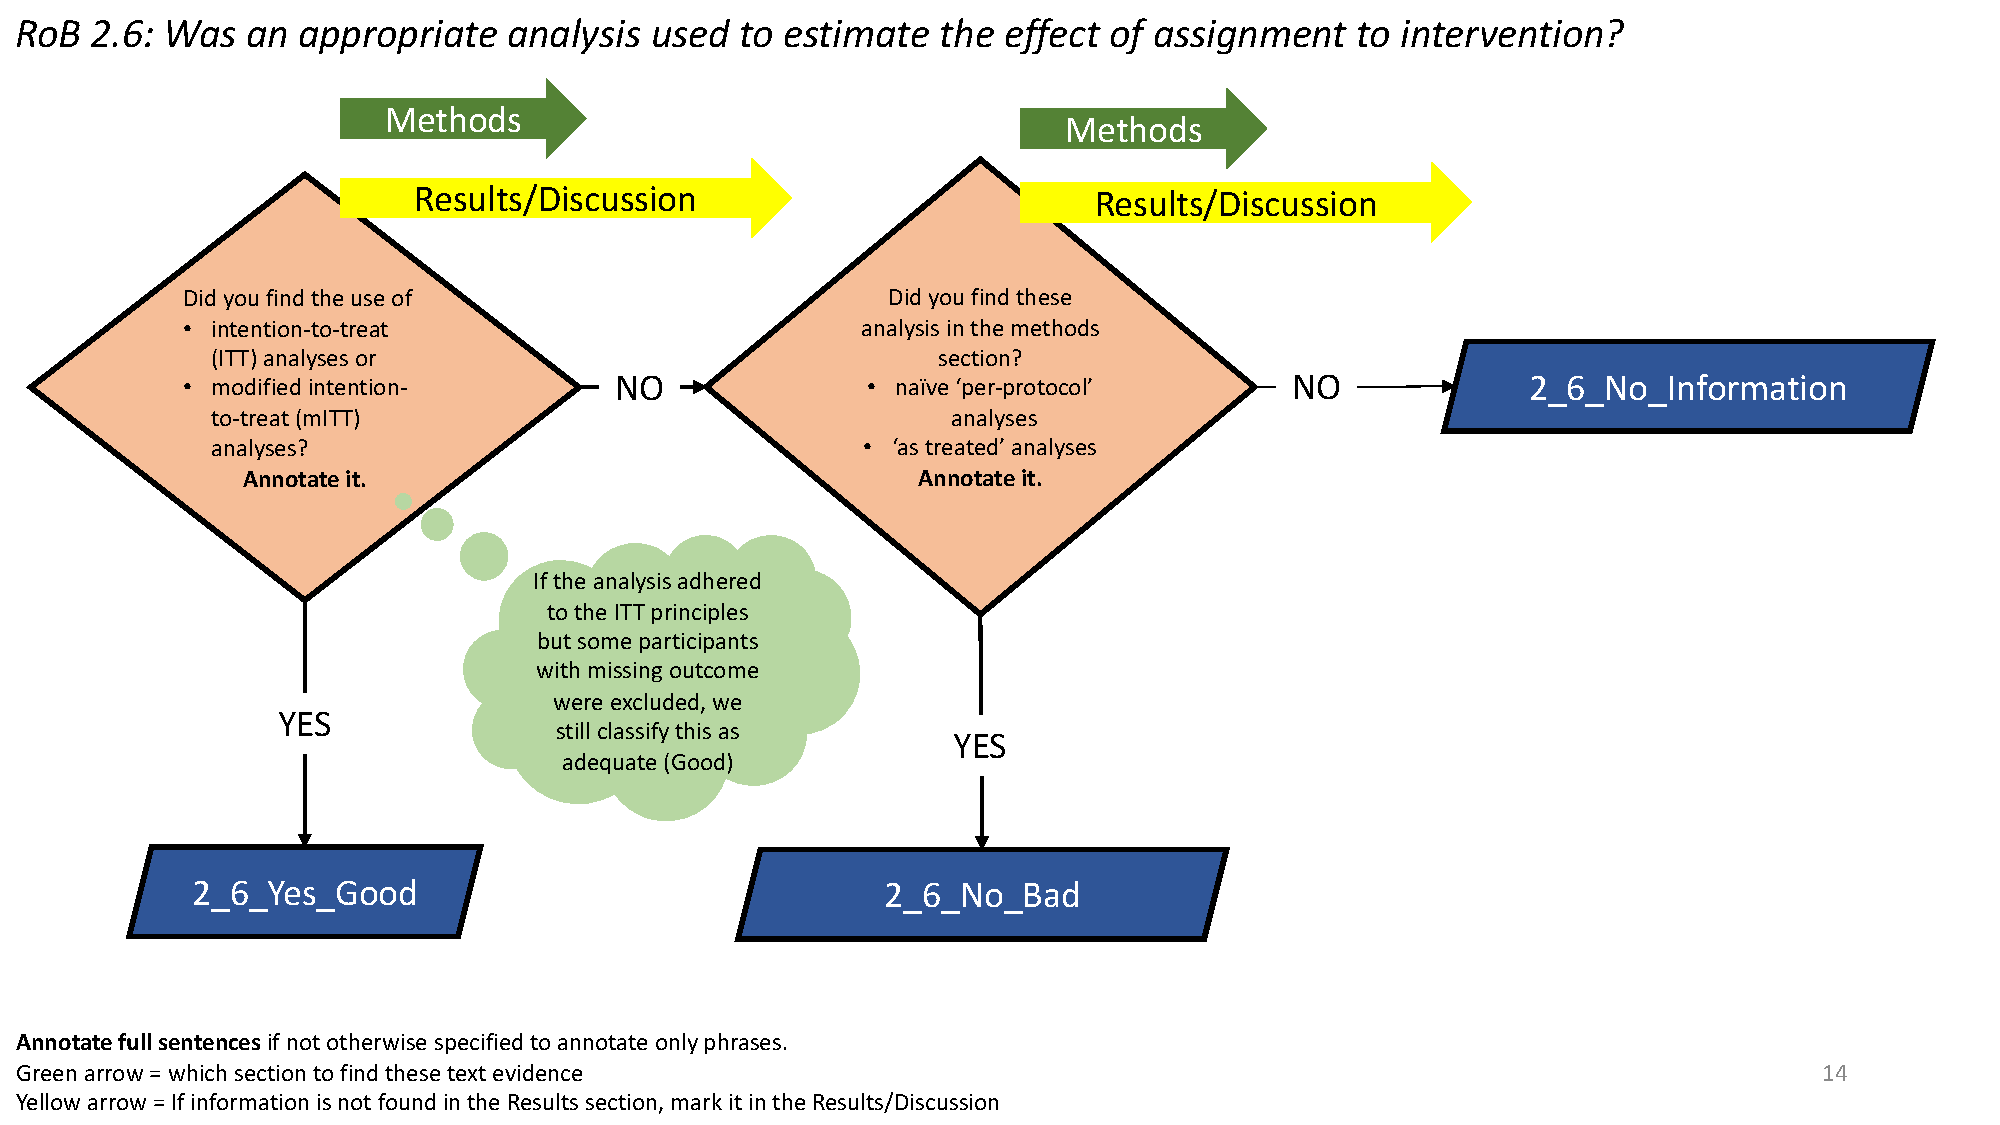
\includegraphics[width=\textwidth]{figures/2_6.pdf}
    \caption{Annotation instructions for the RoB 2.6 signalling question.}
    \label{fig:2_6}
\end{figure}
%
%
%



For annotation instructions regarding the signalling question ``Was an appropriate analysis used to estimate the effect of assignment to intervention?'' please refer to Flowchart~\ref{fig:2_6}.
To clarify, the first diamond in the flowchart guides annotators to identify whether the study used ITT (Intent-to-Treat) or modified ITT analysis.
ITT analysis is a method used to assess the effectiveness of an intervention by analyzing outcomes based on participants' initial assigned treatment group, regardless of whether they actually received the assigned treatment or not.
If the annotators find information indicating the use of ITT analysis, they should mark and label the corresponding sentences as ``2.6 Yes Good''.
Alternatively, if the study did not use ITT analysis and employed methods like naive ``per-protocol'' analysis or ``as treated" analysis to handle deviations from intended interventions, annotators should mark and label the relevant text as ``2.6 No Bad''.
To locate this information, annotators should prioritize checking the Methods section, followed by the Results or Discussion section.
If no information regarding ITT analysis, naive ``per-protocol'' analysis, or ``as treated'' analysis is found, it is assumed that no information is available to answer this question in the paper, and it should be labelled as ``No Information''~\cite{gupta2011intention}.
%
%
%
\subsection*{Signalling question - 2.7 }
\label{subsec:2_7}
%
The question ``Was there potential for a substantial impact (on the result) of the failure to analyze participants in the group to which they were randomized?'' refers to the risk of bias associated with deviations from the intended analysis plan in an RCT.
In an RCT, participants are usually randomized to receive either the intervention being tested or a control intervention.
The analysis plan is typically based on the assumption that all participants will be analyzed according to the group to which they were randomized.
However, there may be instances where participants are not analyzed in the group to which they were randomized, for example, if they dropped out of the study or if they switched groups~\cite{lewis2020dropout,kaufmann1995chapter}. %Kaufmann 1995 has several participants crossover between groups and rates of dropout
This is known as a deviation from the intended analysis plan (not to be confused with deviation from the intended intervention).
The question is asking whether this deviation from the intended analysis plan could have had a substantial impact on the study results.
If there is a potential for a substantial impact, then there is a high risk of bias.
For example, if a large proportion of participants in the intervention group dropped out of the study, but all participants in the control group were analyzed, this could lead to an overestimation of the treatment effect.
Similarly, if participants switched groups, this could lead to an underestimation or overestimation of the treatment effect~\cite{gupta2011intention}.
%Therefore, this question is important for assessing the risk of bias associated with deviations from the intended analysis plan in an RCT, and it helps to ensure that the study results are reliable and valid.


%
%
%
\begin{figure}[hbt]
    \centering
    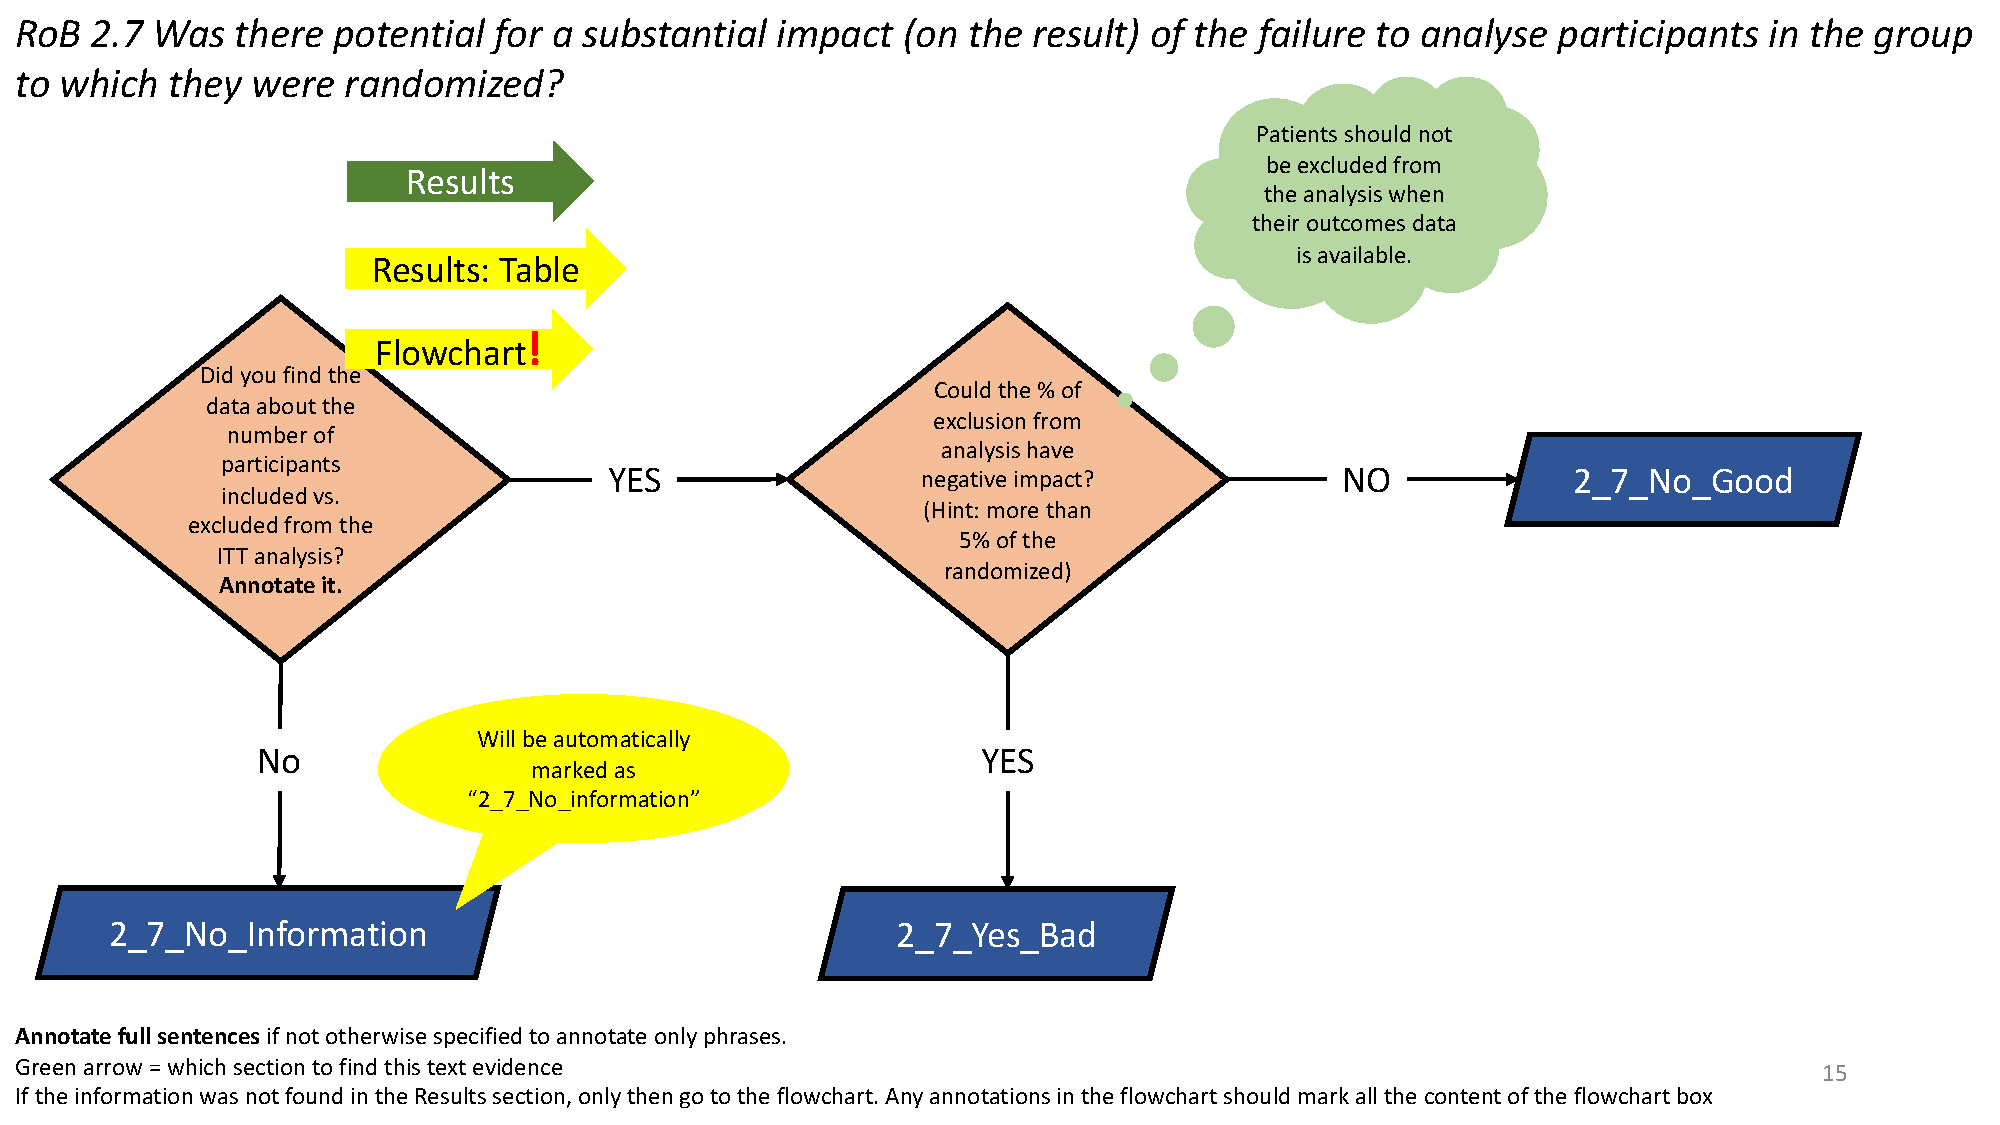
\includegraphics[width=\textwidth]{figures/2_7.pdf}
    \caption{Annotation instructions for the RoB 2.7 signalling question.}
    \label{fig:2_7}
\end{figure}
%
%
%


For annotation instructions for this signalling question, ``Was there potential for a substantial impact (on the result) of the failure to analyse participants in the group to which they were randomized?'' follow the Flowchart~\ref{fig:2_7}.
The analysis we focus on this question is ITT or intent-to-treat analysis.
The first diamond asks the annotators to find the number of people included in the (modified) ITT analysis vs. the number of people randomized to each of the intervention/comparator groups. 
If this information is found, annotate it and follow the ``yes'' flow in the flowchart.
Now examine whether the percentage of participants excluded from the ITT analysis could have had a negative impact.
We also include a hint here, and if more than 5\% of randomized participants were excluded from ITT analysis, the annotators mark the text as ``2.7 Yes Bad'' and ``2.7 No Good'' otherwise.
The first preference to find this information is the Results section.
This information is usually found in the flowcharts, but using our current annotation software, we cannot label the text found in images, and we keep labelling flowcharts as a second priority. 
Therefore, for the sake of simplicity and good agreement, the annotators are requested to mark the flowchart captions.
If the information is not found in the results section, mark the text in the table.
If the information is to be found nowhere except in a flowchart, mark the caption of the flowchart.
However, ensure that the flowchart annotation is your last resort.
%If you find it in the flowchart, mark the caption and also ``included n=XX for ITT''. % Unfortunately, you cannot mark the flowchart because the new tool does not allow image annotation
%Sometimes, there could be disagreements here. Let's take, for example, Solomons\_2020\_VISA\_A\_12months\_IAA\_Hilfiker\_Sattelmayer\_with\_Protocol.pdf where Martin marks "We did not impute or replace any missing values but rather fitted all the available data to the model" as No good. 
%However, what does the phrase "all the available data" mean? Maybe only 70\% of the outcomes data was available.
%
%
%
%%%%%%%%%%%%%%%%%%%%%%%%%%%%%%%%%%%%%%%%%%%%%%%%%%%%%
\section*{Annotation Guidelines for RoB domain 3}
\label{sec:dom3}
%%%%%%%%%%%%%%%%%%%%%%%%%%%%%%%%%%%%%%%%%%%%%%%%%%%%%
%
Domain 3 of the Revised Cochrane Risk of Bias (RoB) 2 tool addresses the potential ``Bias due to missing outcome data'' in a study.
Bias due to missing outcome data refers to situations where the data for some participants are not available for analysis, and this missingness may be related to the outcomes being measured.
This domain aims to evaluate whether there is a potential bias in how missing data is handled and reported, which can affect the validity and reliability of the RCT's findings.
%
%
%
\subsection*{Signalling question - 3.1 }
\label{subsec:3_1}
%
The question ``Were data for this outcome available for all, or nearly all participants randomized?'' assesses the completeness of outcome data in a study.
It aims to determine if data for the specific outcome of interest were collected and available for analysis for a high proportion of the participants who were initially randomized into the study.
By evaluating this question, you can assess the risk of bias associated with missing or incomplete outcome data.
If the data for the outcome of interest were not available for a substantial number of participants or if there was a high degree of missing data, it raises concerns about the potential impact on the validity and reliability of the study's findings.
Missing data can lead to reduced statistical power and imprecise estimates of treatment effects
Adequate availability of outcome data for the majority of randomized participants enhances confidence in the study's results and reduces the risk of bias in this domain~\cite{gnang2020empirical,shara2015randomly}.


%
%
%
\begin{figure}[hbt]
    \centering
    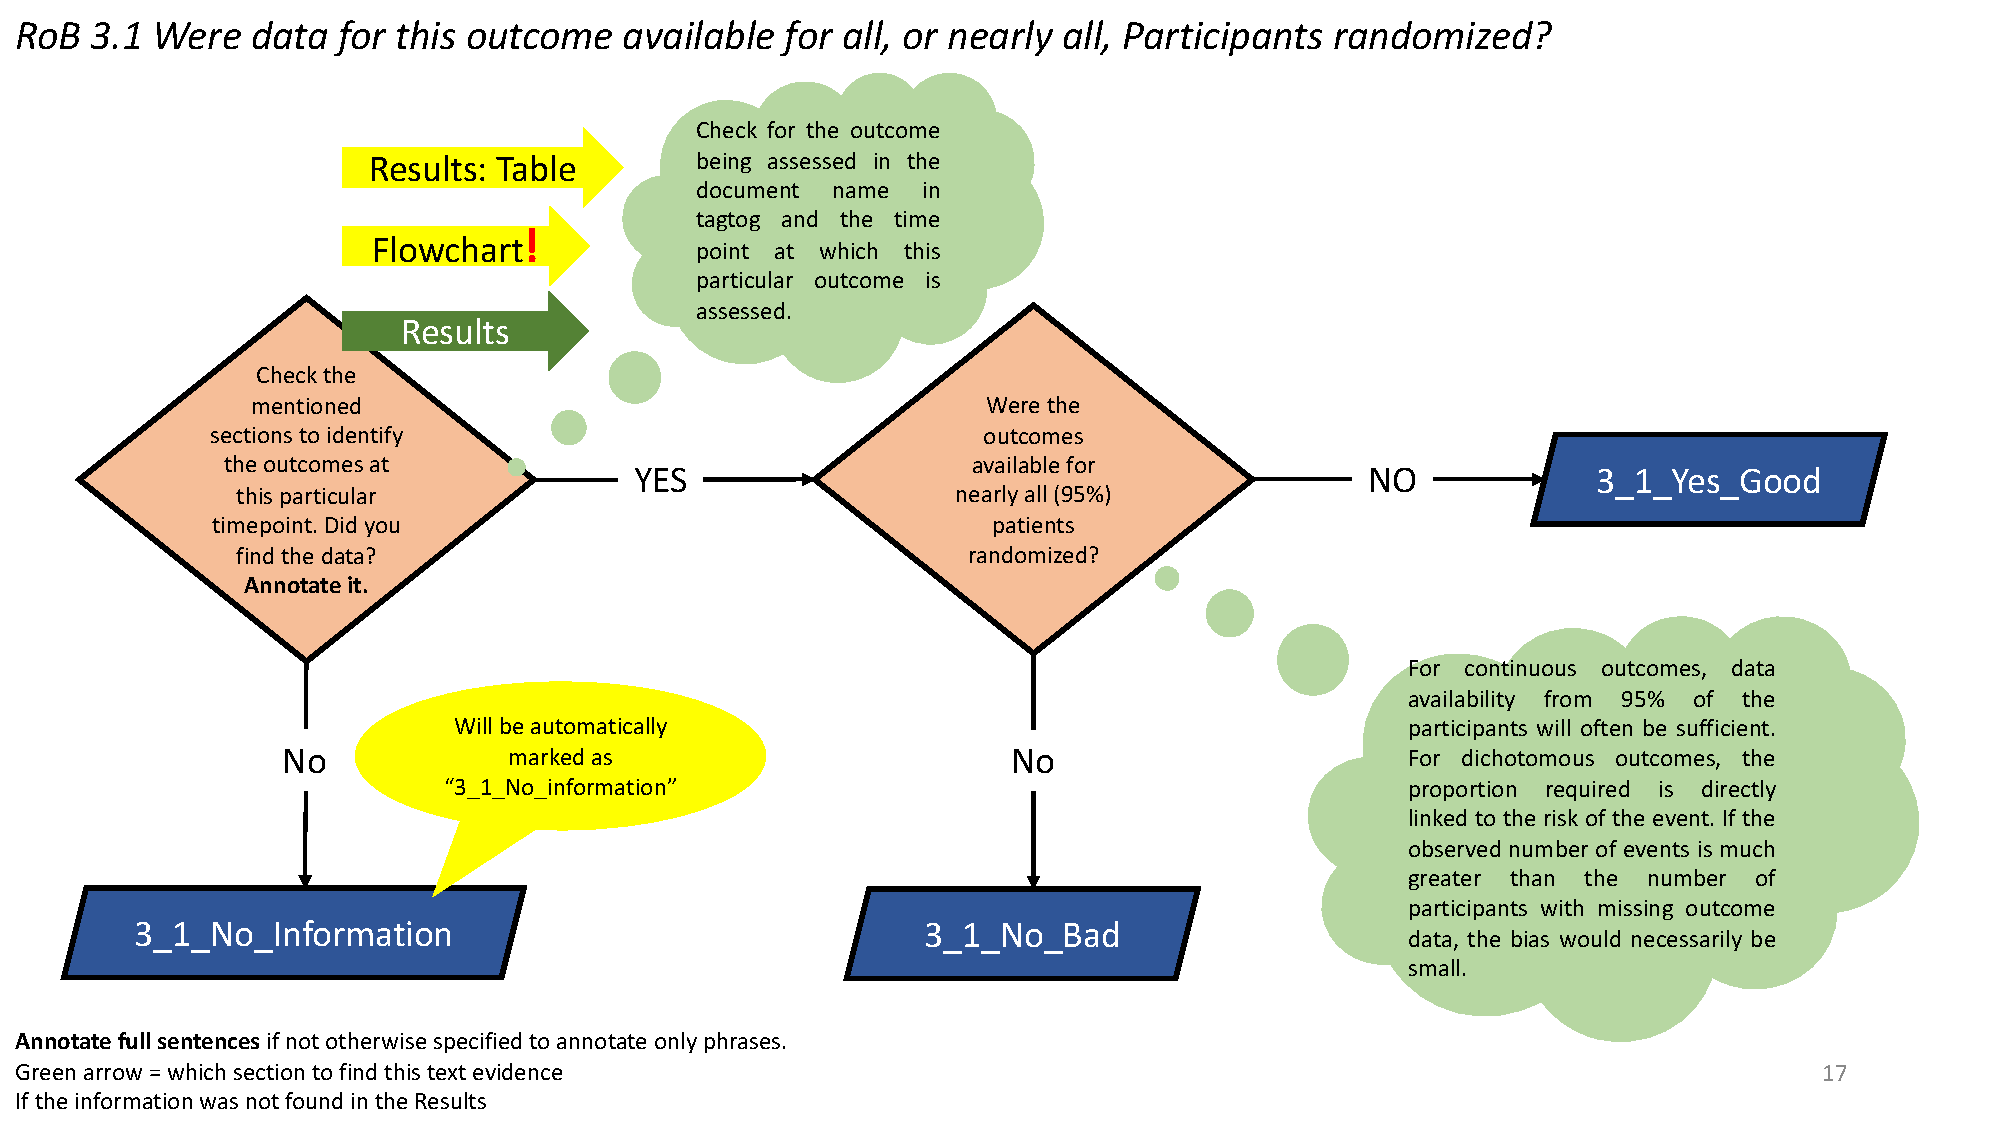
\includegraphics[width=0.95\textwidth]{figures/3_1.pdf}
    \caption{Annotation instructions for the RoB 3.1 signalling question.}
    \label{fig:3_1}
\end{figure}
%
%
%


For annotation instructions for this signalling question, ``Were data for this outcome available for all, or nearly all Participants randomized?'' follow the Flowchart~\ref{fig:3_1}.
Following the above explanation, the first diamond instructs the annotators to check the Results section (first priority) and the flowchart (second priority) to identify outcome data at the specific time point of interest.
If the annotators find that the outcomes data were available for all or nearly all (at least 95\% of the total) participants, mark the text descriptions mentioning it and label it with ``3.1 Yes Good''.
If the outcomes data were available for less than 95\% of participants randomized, then mark this information and label it with ``3.1 No Bad''.
If no information regarding the availability of outcome data at the specified time point is found, consider the question as having ``No Information''.
This information is likely found in the Results section of the RCT under consideration, but if not found there, then mark the information in results table. 
If the information is to be found nowhere except in a flowchart, mark the caption of the flowchart.
However, ensure that the flowchart annotation is your last resort.
%
%
%
\subsection*{Signalling question - 3.2 }
%
The signalling question ``Is there evidence that the result was not biased by missing outcome data?'' evaluates the potential bias introduced by missing data in a study.
It aims to evaluate whether there is sufficient evidence to conclude that the study's results were not influenced or biased due to missing outcome data.
When answering this question, researchers evaluate whether the missing outcome data could have influenced the study's results in a biased manner.
Missing outcome data can occur when participants drop out of a study, fail to provide data for certain outcomes, or when data is not collected as planned.
The concern is that the missing data may introduce bias if it is related to the treatment being studied or if it differs systematically between the treatment groups~\cite{akl2012potential}.
To determine if there is evidence that the result was not biased by missing outcome data, researchers typically assess the amount of missing data and whether it is evenly distributed across different study groups.
If there is a significant amount of missing data, especially if it is related to the outcomes being measured, it may increase the risk of bias.
Researchers evaluate the strategies employed to handle missing data.
This may involve techniques such as imputation (replacing missing values with estimated values) or sensitivity analyses to assess the impact of missing data on the results.
To annotate for this signalling question, the annotators should specifically look for the analysis method that was used to handle or correct for the missing outcomes data.
This analysis method could be, for example, Multiple Imputation (MI), Inverse Probability Weighting (IPW), Weighted Estimating Equations (WEE), and Pattern Mixture Models (PMM)~\cite{bell2014handling,khan2021missing}.


%
%
%
\begin{figure}[hbt]
    \centering
    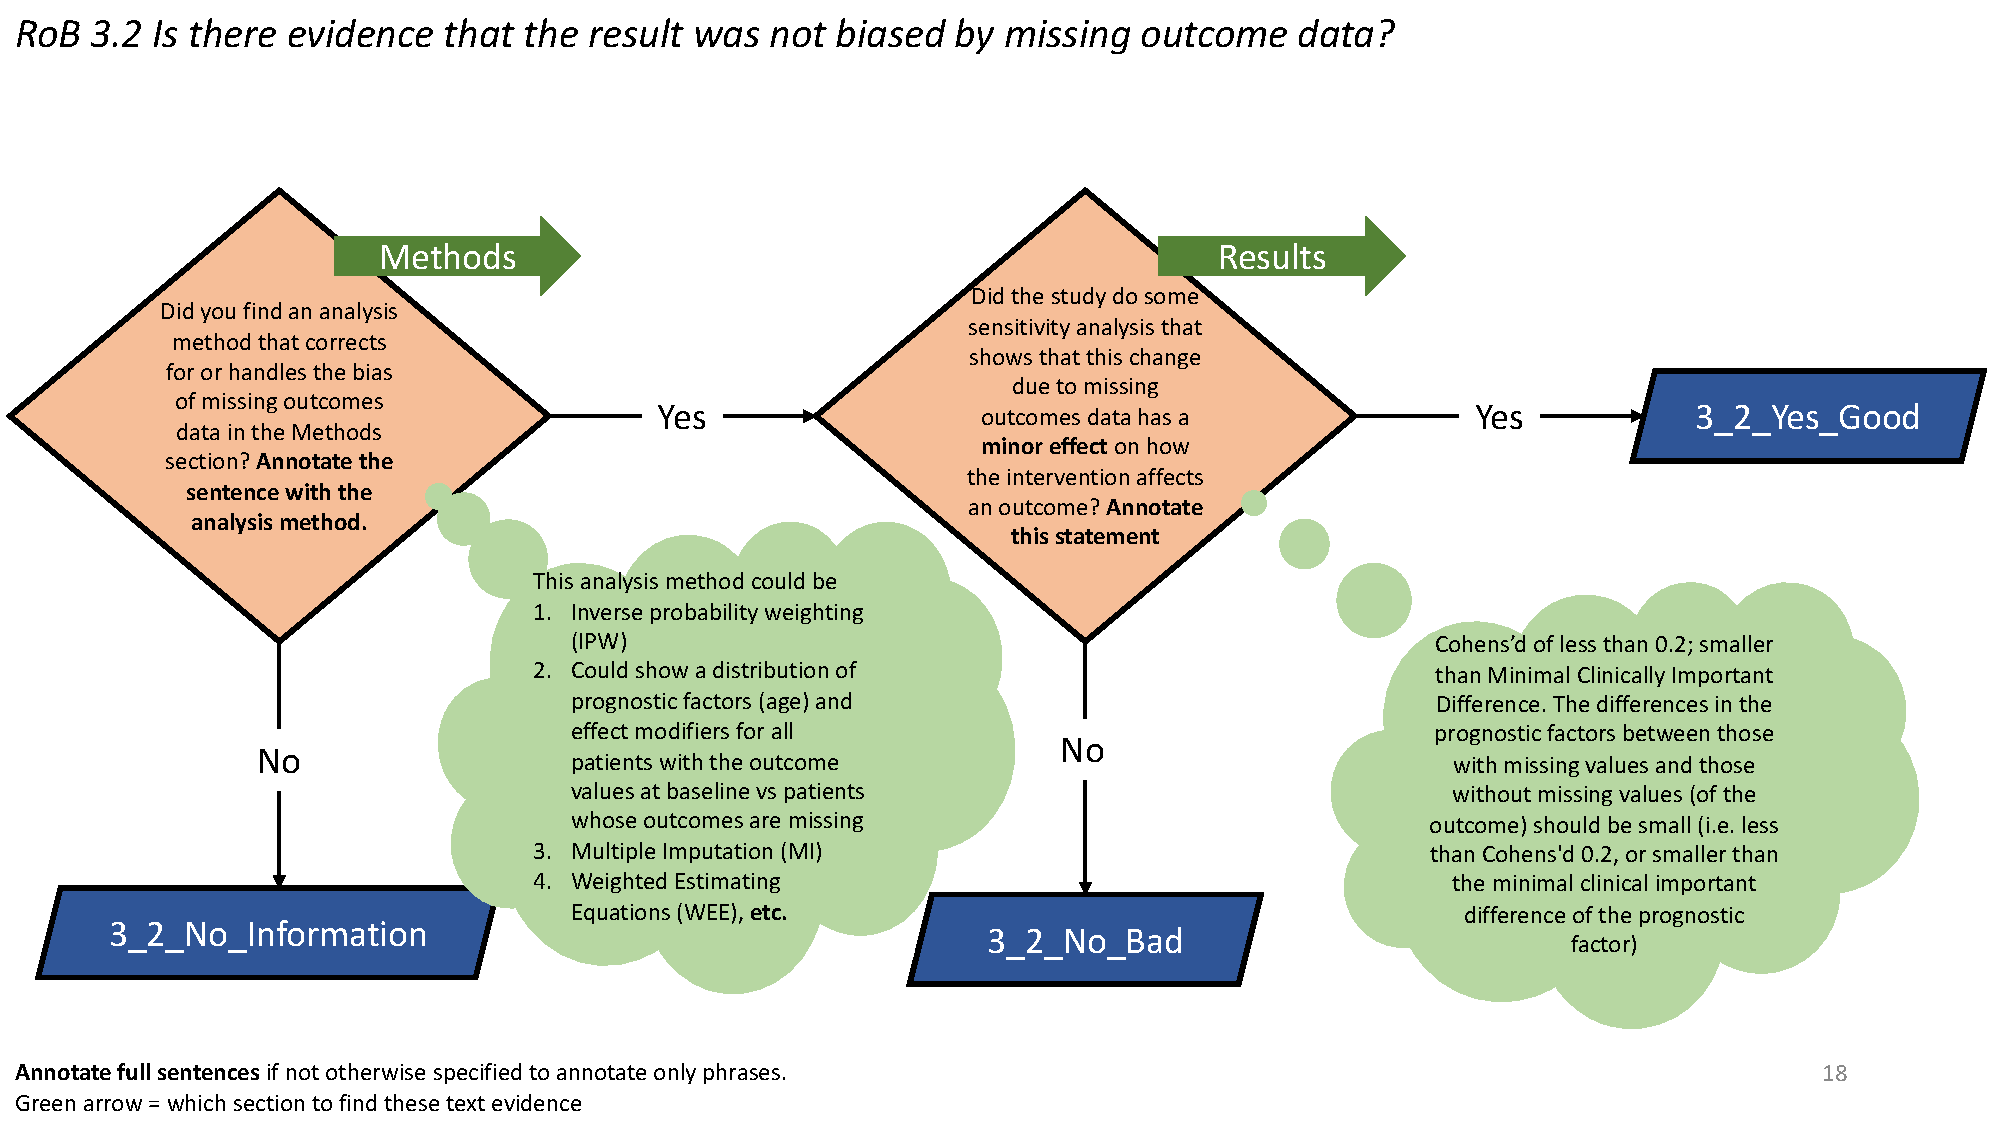
\includegraphics[width=0.95\textwidth]{figures/3_2.pdf}
    \caption{Annotation instructions for the RoB 3.2 signalling question.}
    \label{fig:3_2}
\end{figure}
%
%
%


For annotation instructions for this signalling question, ``Is there evidence that the result was not biased by missing outcome data?'' follow the Flowchart~\ref{fig:3_2}.
The first diamond asks the annotators to look for the use of one of these methods: Multiple Imputation (MI), Inverse Probability Weighting (IPW), Weighted Estimating Equations (WEE), and Pattern Mixture Models (PMM).
If the use of the analysis method is found, go to the next diamond, which instructs the annotator to identify any method that was used to conduct sensitivity analysis~\cite{goldberg2021data}.
Did the study do some sensitivity analysis that shows that this change is due to missing outcomes data, or did the different analysis methods used have a minor effect on how the intervention affects an outcome?
Then annotate these sentences containing the analysis method and sensitivity analysis and mark them with ``3.2 Yes Good''.
By conducting sensitivity analyses, researchers can gain insight into the potential impact of missing data on the study's findings. This information helps to address concerns regarding bias and strengthens the overall validity and reliability of the study results.
If no sensitivity analysis was done, then mark the sentence containing the method used to handle the missing data and label it as ``3.2 No Bad''.
The information to answer this signalling question is likely found in the Method section of the RCTs.

%
%
%
\subsection*{Signalling question - 3.3 }
\label{subsec:3_3}
%
The question ``Could the missingness in the outcome depend on its true value?'' assesses the potential for missing outcome data to be related to the actual values of the outcome variable.
This question aims to evaluate whether the missingness of data is related to the true values of the outcome being measured in a study.
By considering this question, you are examining whether there is a possibility that the missingness of outcome data is not random but instead depends on the actual values of the outcome variable.
If missingness is related to the true values, it can introduce bias and impact the validity of the study's results~\cite{bell2014handling,calvert2013reporting}.
To answer this question, reviewers need to assess whether there is a potential relationship between the missing data and the true value of the outcome.
This can be done by examining the reasons for missing data and analyzing whether the missing data is related to other participant characteristics or study factors.
For example, if the study assesses fatigue as the outcome of interest and if participants experience fatigue or drop out of the study due to fatigue, the missingness can potentially be related to missing outcome data in a study.
If the answer to RoB 3.3 is judged as ``low risk of bias'' it means that there is little risk that the missing data could have biased the study findings.
If the answer is ``high risk of bias'' it means that there is a significant risk of bias due to missing outcome data, and the study results should be interpreted with caution.


%
%
%
\begin{figure}[hbt]
    \centering
    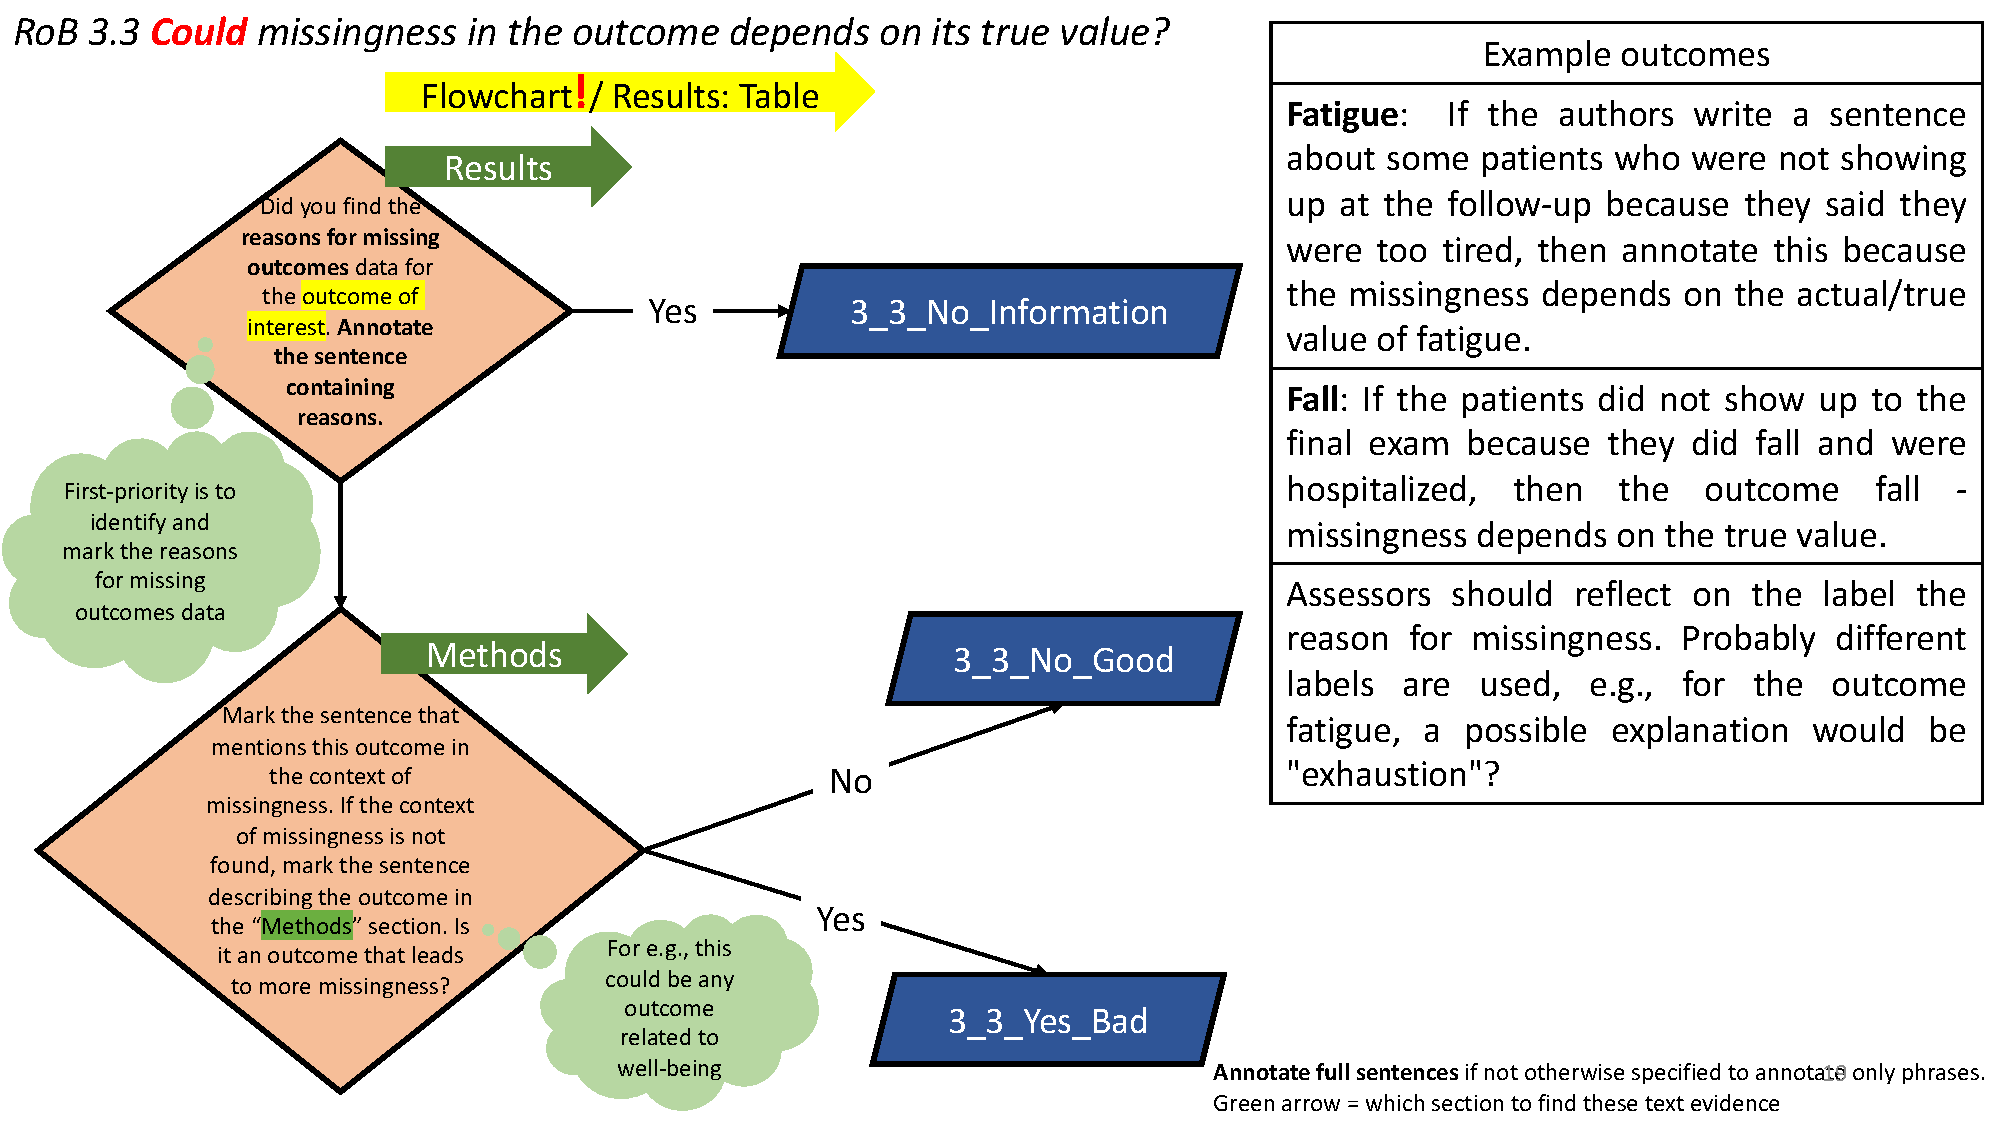
\includegraphics[width=\textwidth]{figures/3_3.pdf}
    \caption{Annotation instructions for the RoB 3.3 signalling question.}
    \label{fig:3_3}
\end{figure}
%




For annotation instructions for this signalling question, ``RoB 3.3 Could missingness in the outcome depends on its true value?'' follow the Flowchart~\ref{fig:3_3}.
In order for the annotator to answer this signalling question, the first diamond request the annotators to find the reasons for missing outcomes data.
If found the reason for missing outcomes data or not, go to the next diamond and which requests you to find, and if found, mark the sentences that mention this outcome in the context of missingness.
If this is an outcome that leads to missingness, then label the marked text as ``3.3 Yes Bad''.
Otherwise, if no such sentences with missingness context were identified, then mark the sentence describing the outcomes assessed in the Methods section and mark the sentence.
If this is an outcome that leads to missingness, then label the marked text as ``3.3 Yes Bad''.
This is a theoretical question, the answer to which could be basically obtained just by knowing what outcomes are being assessed in the RCT.
%
%
%
\subsection*{Signalling question - 3.4 }
\label{subsec:3_4}
%
The question ``Is it likely that the missingness in the outcome depended on its true value?'' assesses the likelihood of missing outcome data to be related to the actual values of the outcome variable.


For annotation instructions for this signalling question, ``RoB 3.4 Is it likely that missingness in the outcome depended on its true value?'' follow the Flowcharts~\ref{fig:3_4_1}~\ref{fig:3_4_2}~\ref{fig:3_4_3}~\ref{fig:3_4_4}.
To answer this question, the annotator should first find the numbers for missing outcome data in both the intervention and control arms at the specified time point.
If these numbers are found, check if the percentage of missing outcome data is greater than 5\% between randomization and the analysis time point.
If the difference exceeds 5\%, mark the corresponding description where these numbers are mentioned and label it as ``3.4 Yes Bad'', and otherwise label it as ``3.4 No Good''.
Ideally, a randomized controlled trial (RCT) should mention if the difference between the patients randomized and those whose outcomes were analyzed is greater than 5\%.
If such information is found, mark it.
If there is no explicit text mentioning this, mark the proportions.
This information is usually located in the Results section text or possibly in a table. It may also be identified in the flowchart, but the flowchart should be used as a last resort.
If the numbers regarding missing outcomes data are not found then, go to the Flowchart~\ref{fig:3_4_2}.


%
%
%
\begin{figure}[hbt]
    \centering
    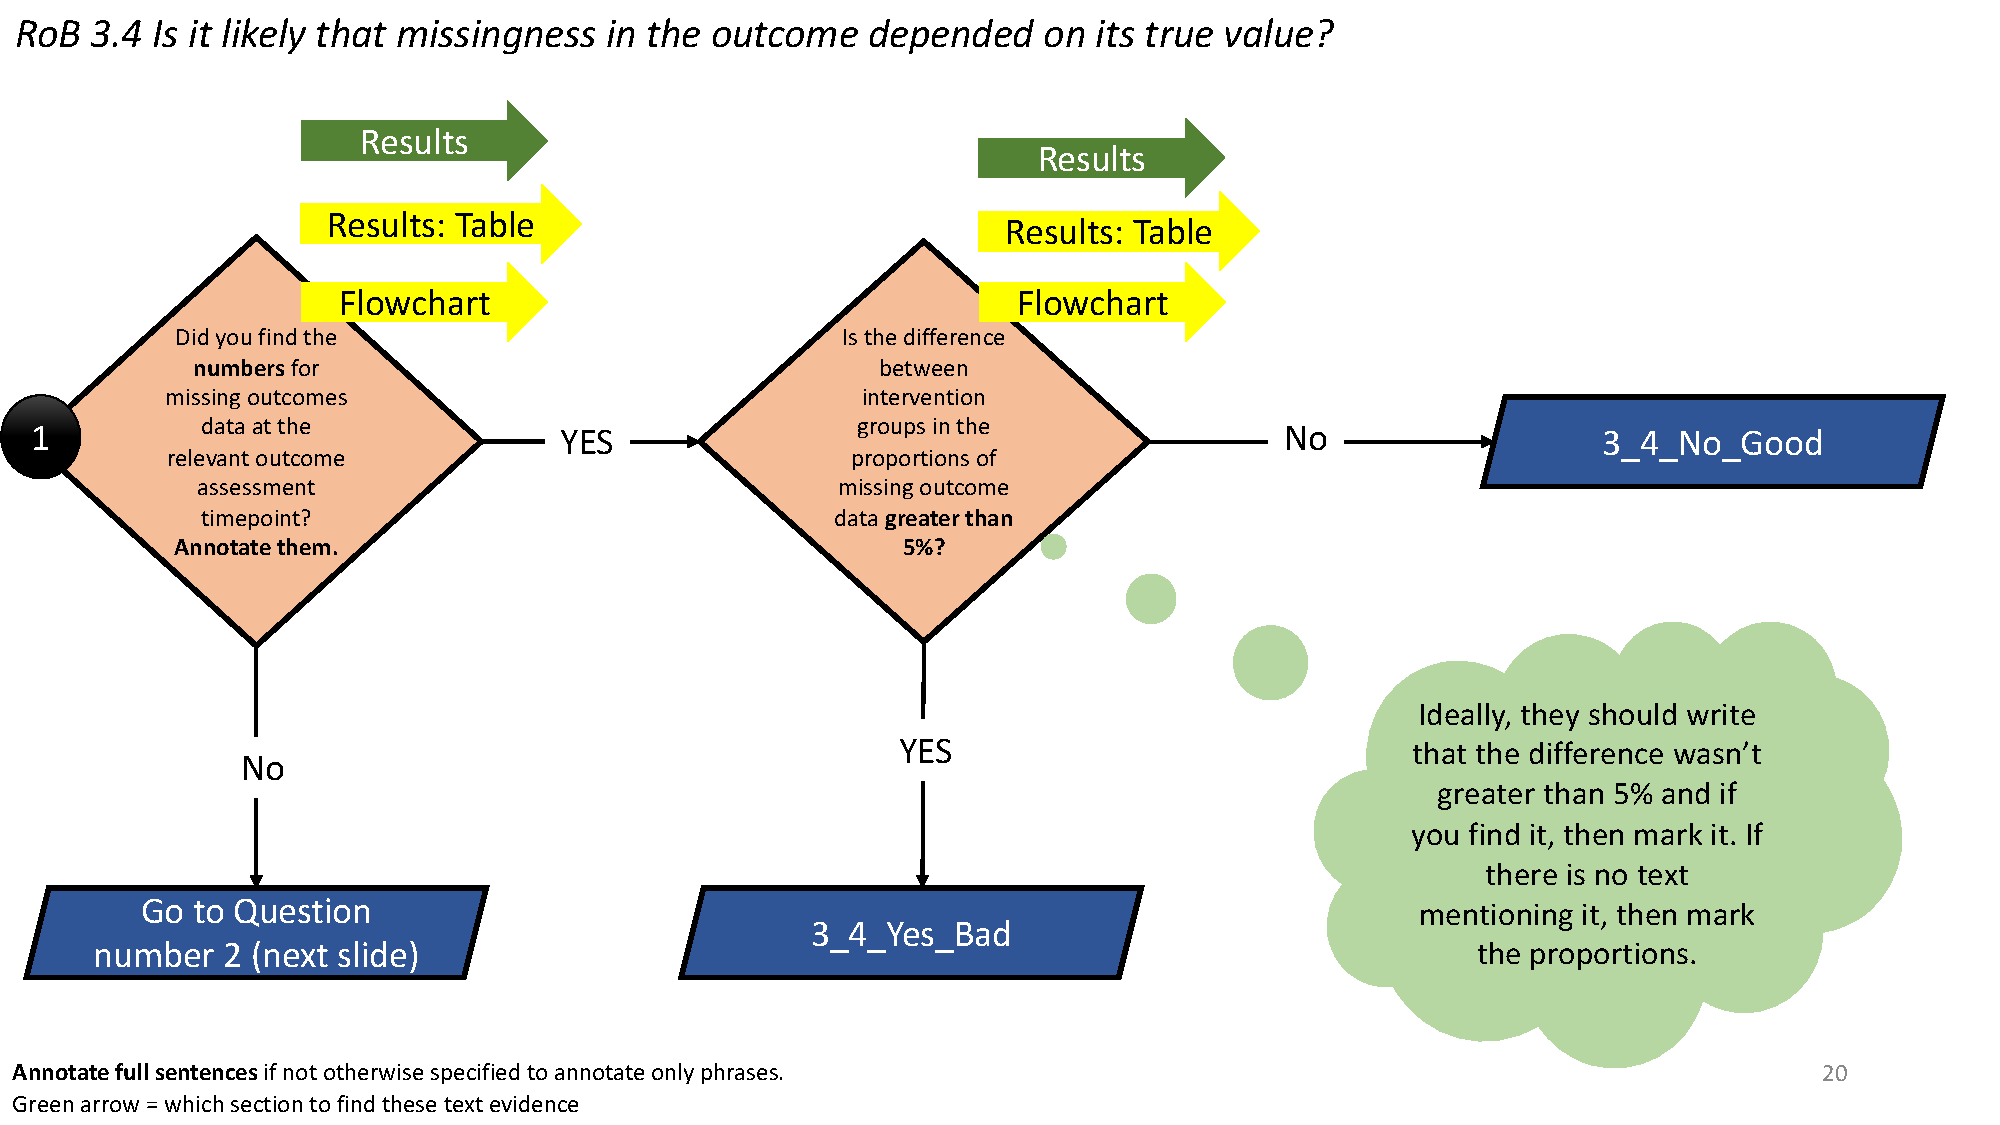
\includegraphics[width=\textwidth]{figures/3_4_1.pdf}
    \caption{Annotation instructions for the RoB 3.4 signalling question.}
    \label{fig:3_4_1}
\end{figure}


\begin{figure}[hbt]
    \centering
    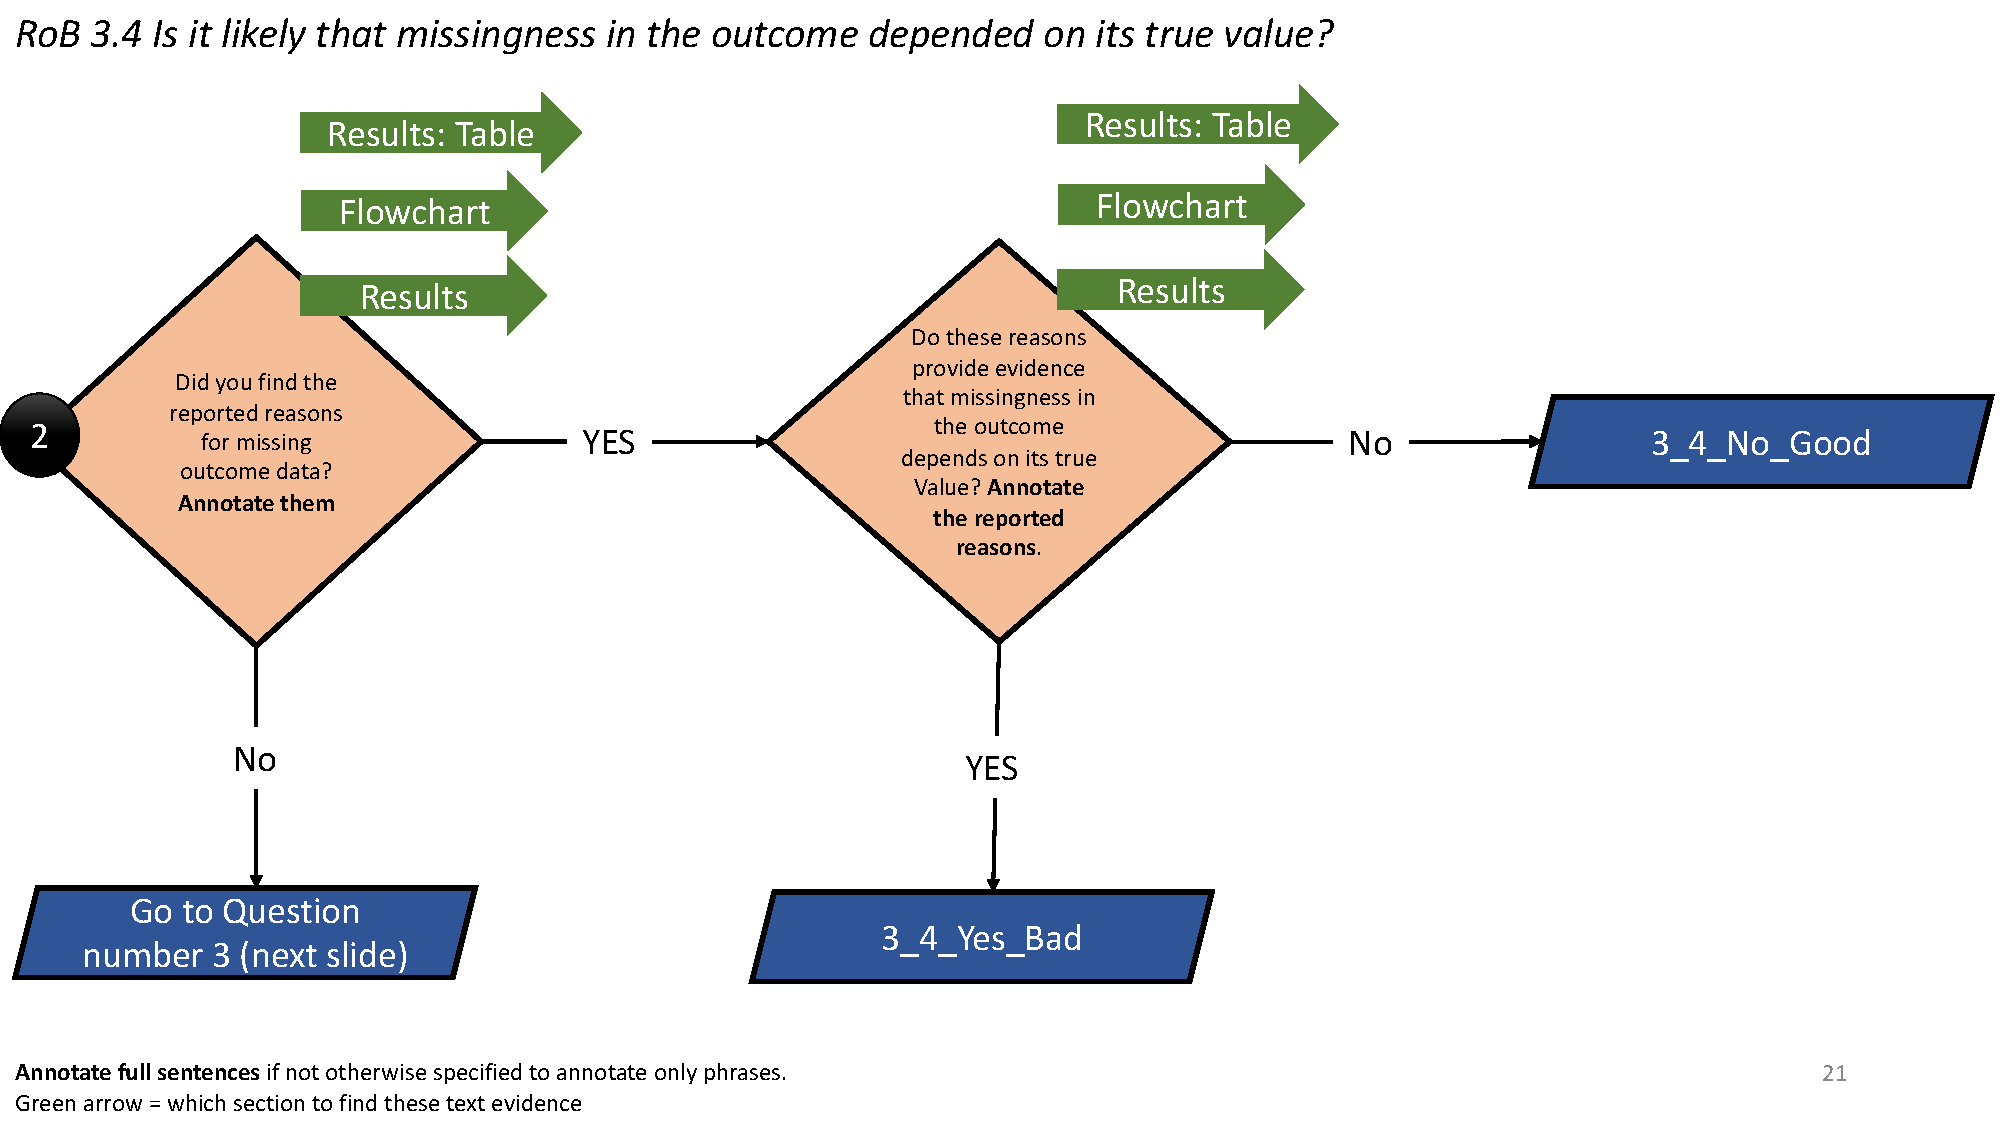
\includegraphics[width=\textwidth]{figures/3_4_2.pdf}
    \caption{Annotation instructions for the RoB 3.4 signalling question.}
    \label{fig:3_4_2}
\end{figure}


\begin{figure}[hbt]
    \centering
    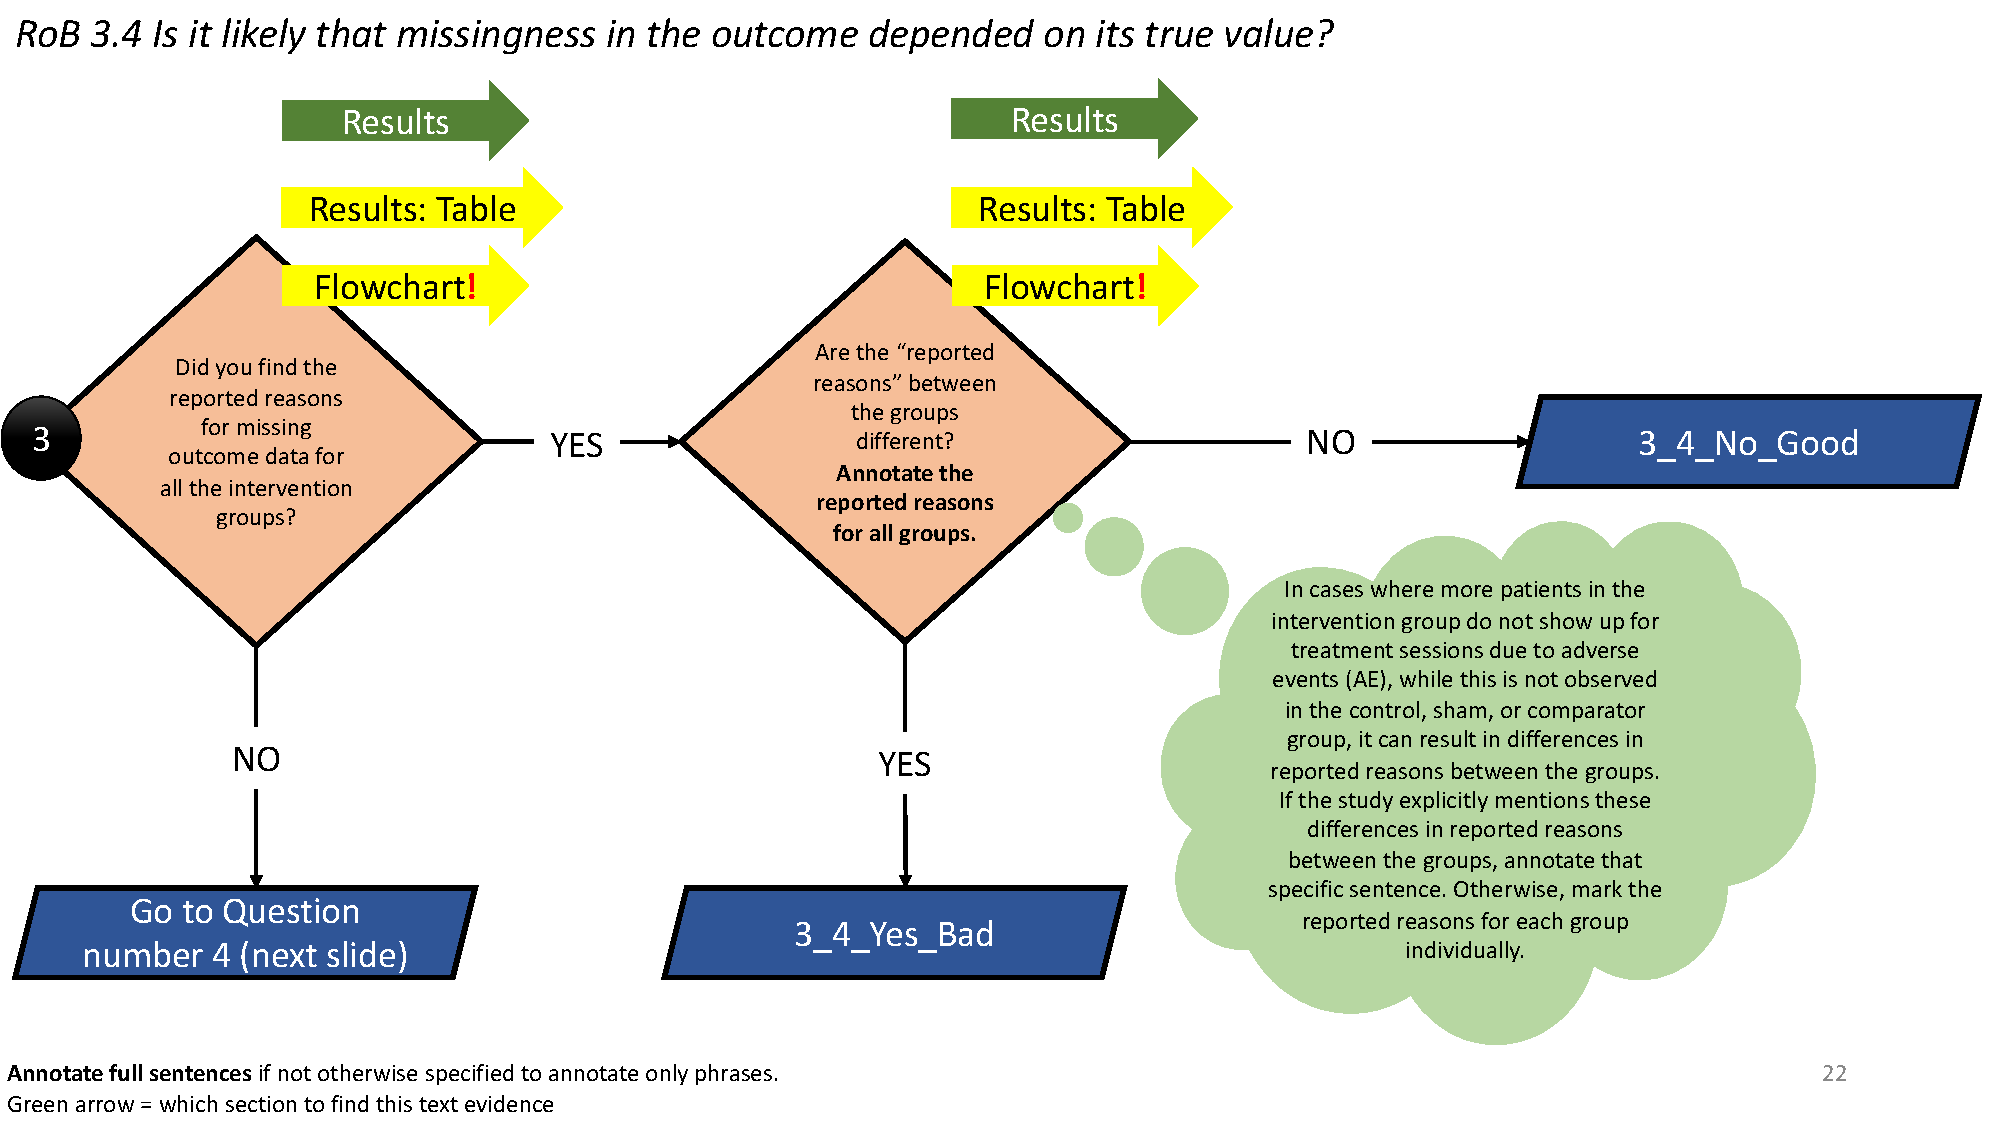
\includegraphics[width=\textwidth]{figures/3_4_3.pdf}
    \caption{Annotation instructions for the RoB 3.4 signalling question.}
    \label{fig:3_4_3}
\end{figure}


\begin{figure}[H]
    \centering
    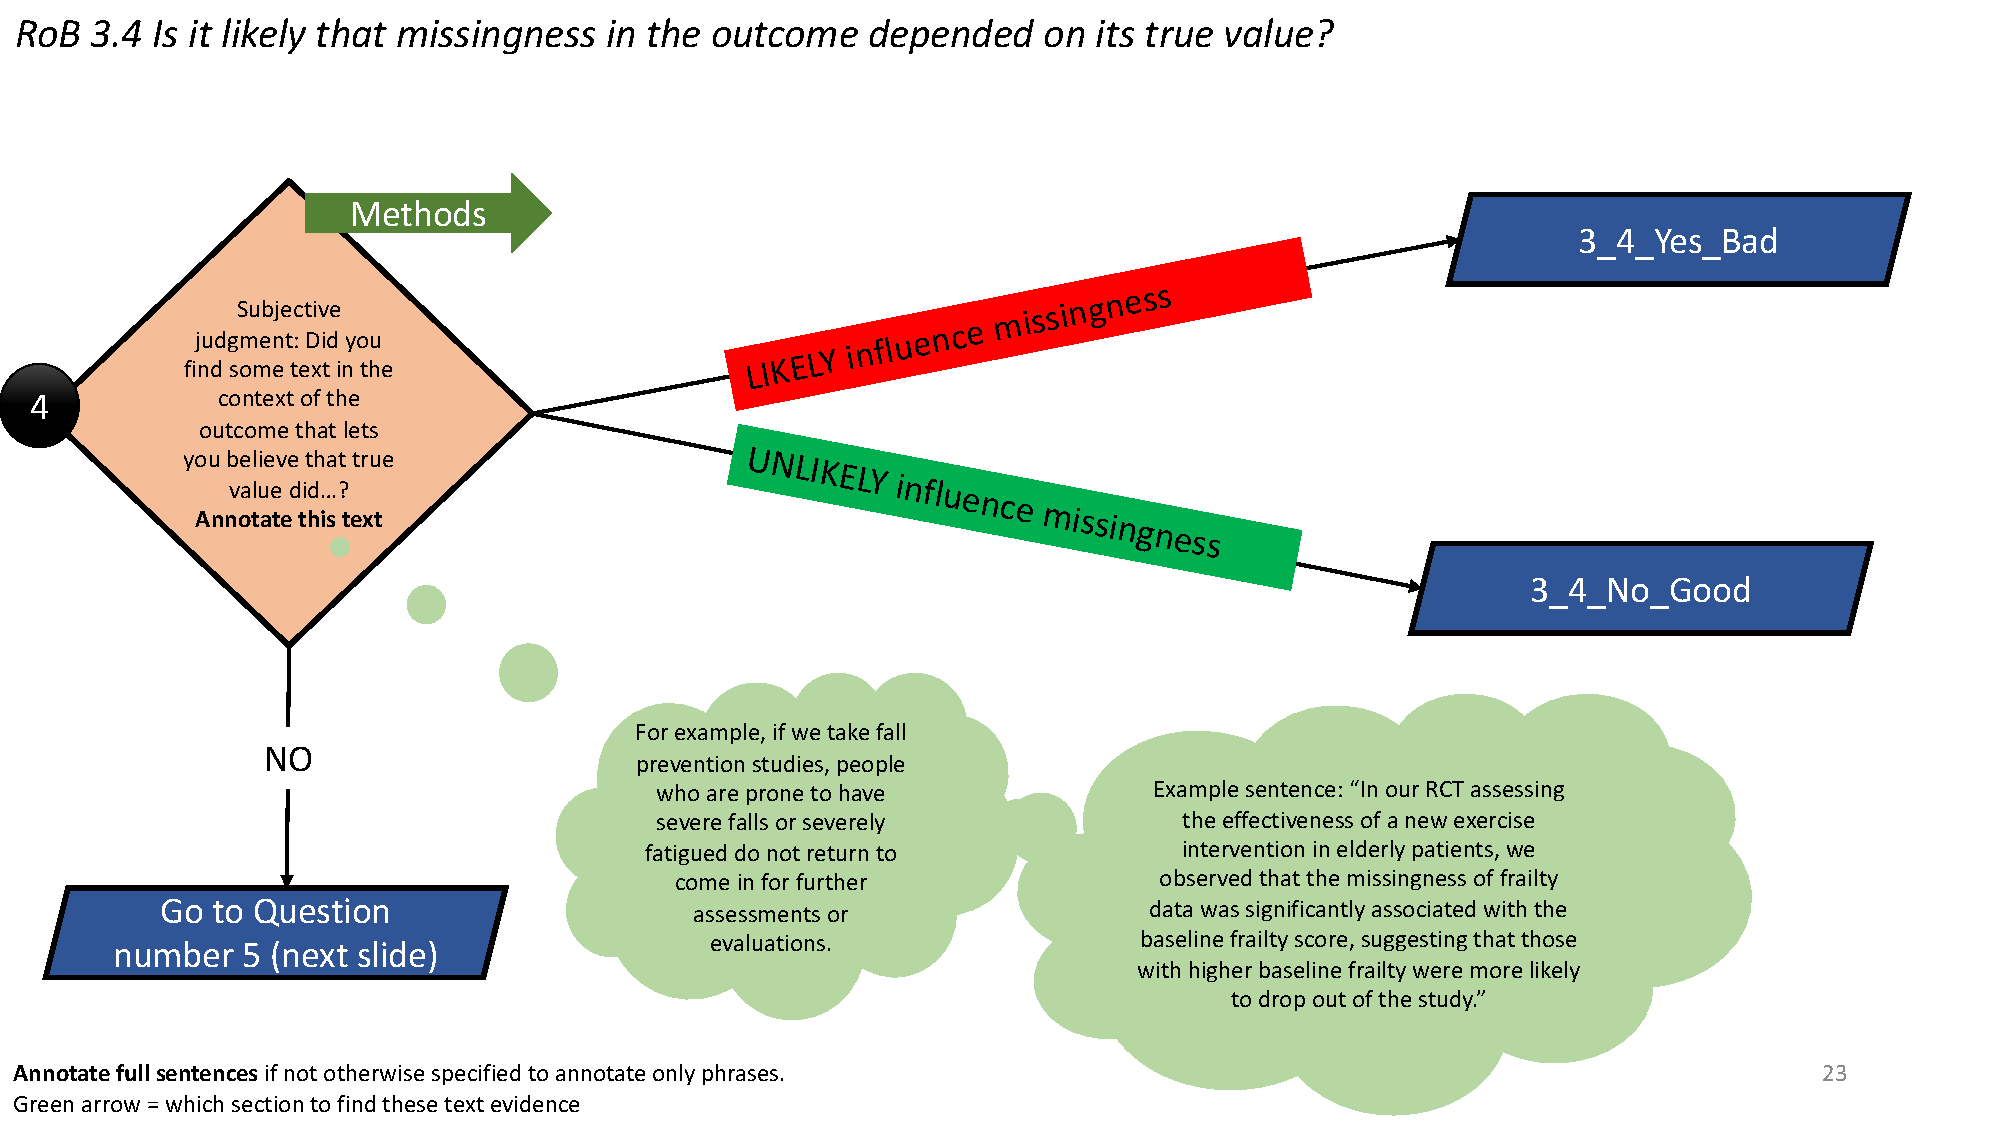
\includegraphics[width=\textwidth]{figures/3_4_4.pdf}
    \caption{Annotation instructions for the RoB 3.4 signalling question.}
    \label{fig:3_4_4}
\end{figure}


\begin{figure}[H]
    \centering
    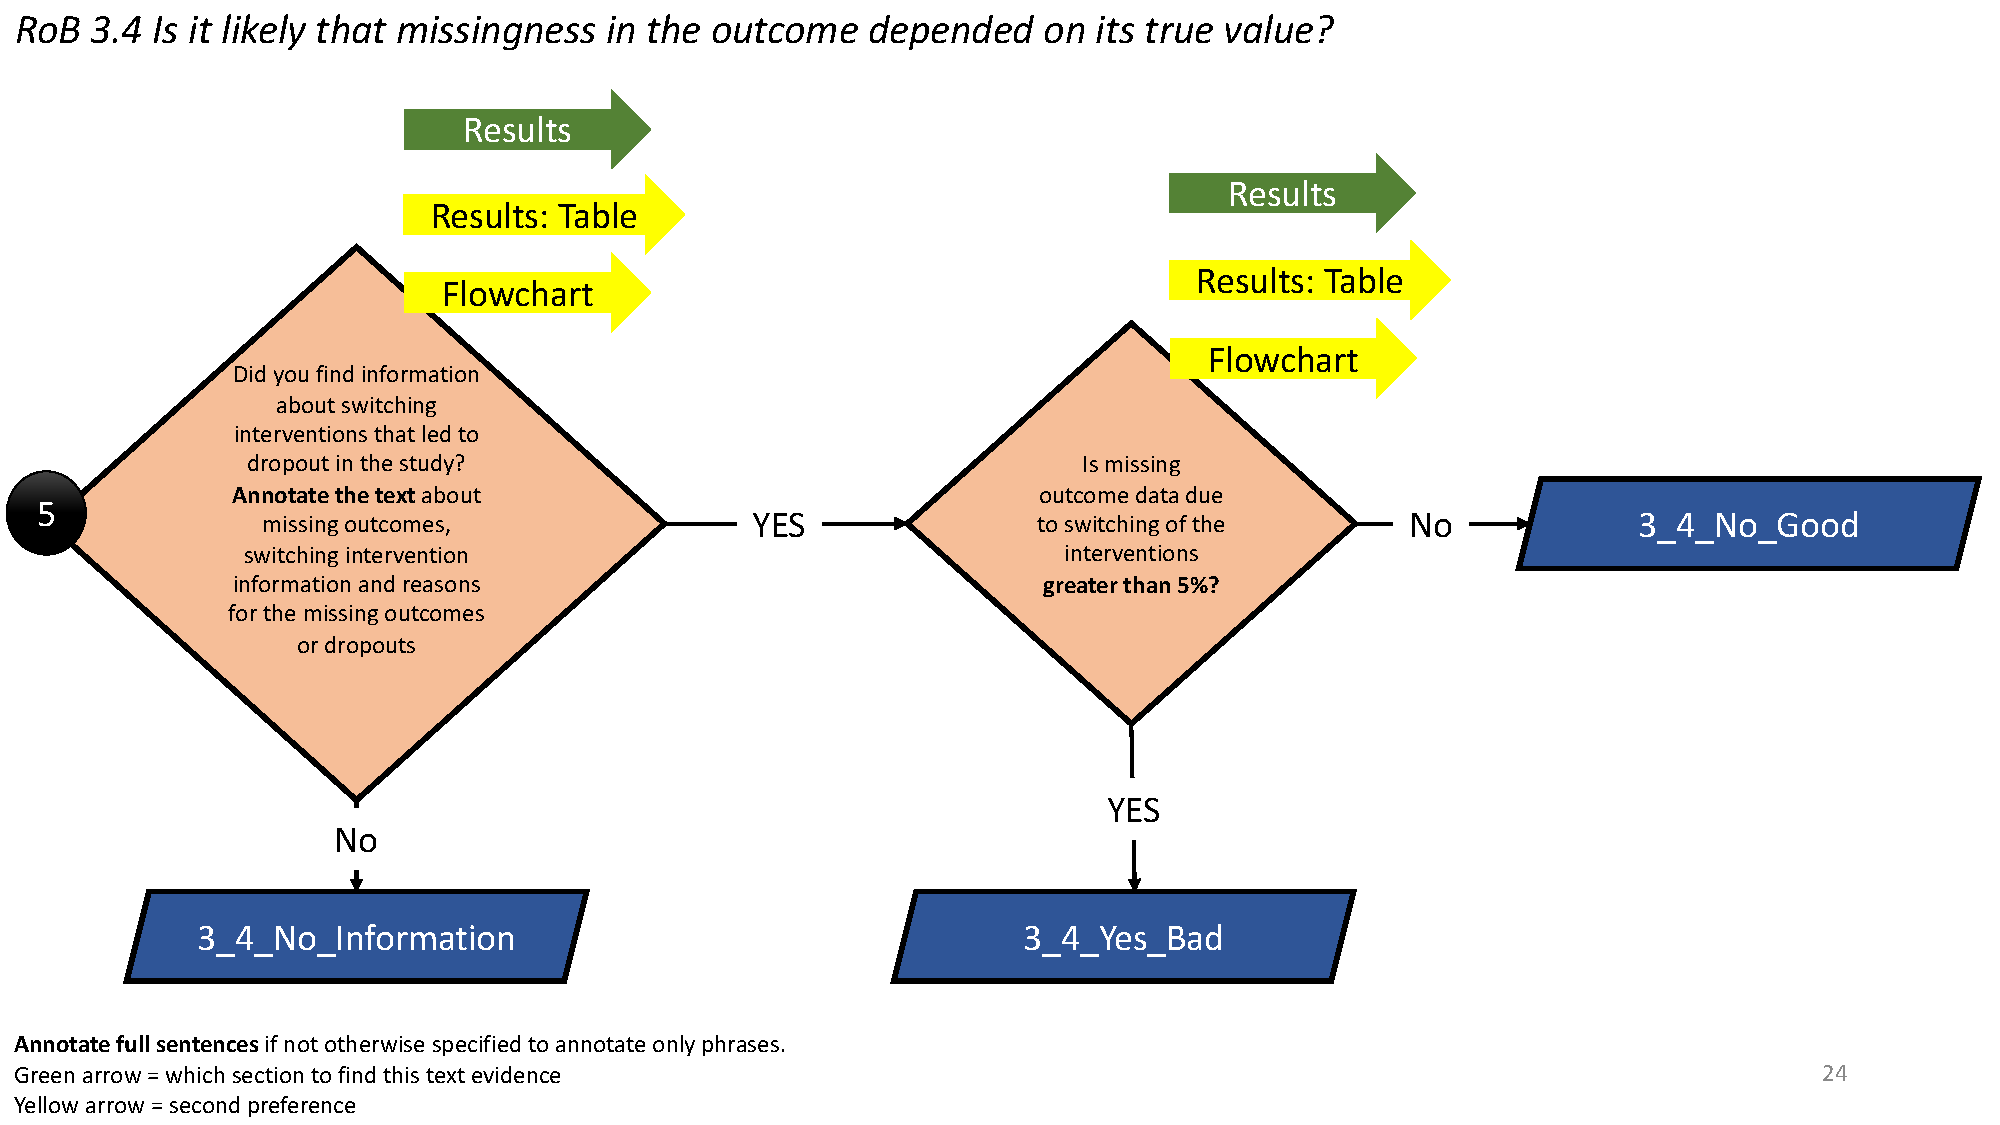
\includegraphics[width=\textwidth]{figures/3_4_5.pdf}
    \caption{Annotation instructions for the RoB 3.4 signalling question.}
    \label{fig:3_4_5}
\end{figure}
%
%
%

The Flowchart~\ref{fig:3_4_2} find the reported reasons for missing outcome data, if available, and annotate them.
If these reasons indicate that missingness in the outcome DOES NOT depend on its true value, follow the "no" route and label the reason as ``3.4 No Good''.
If the missingness in the outcome DOES depend on its true value then follow the connector route ``yes'' and label the reason with ``3.4 Yes Bad''.
Again, this information is likely to be found in the Results section text or probably in the table. 
It can also be identified in the flowchart, but flowchart should be the last resort.


Even if the reported reasons for missingness are found, proceed to Flowchart~\ref{fig:3_4_3} and determine if these reported reasons differ between the intervention groups.
If the reported reasons are different across the intervention groups, mark them and label them as ``3.4 Yes Bad'', and if the reported reasons across the groups are similar then mark them and label with ``3.4 No Good''.
Next, go to Flowchart 4~\ref{fig:3_4_4} and search for text descriptions related to the outcome that suggest the true value could influence missingness.
If such text is found, highlight it and label it as ``3.4 Yes Bad''.
If the text suggests that the true value could not influence missingness, mark it and label it as ``3.4 No Good''.
Regardless of the label choice, go to the next Flowchart~\ref{fig:3_4_4}.
The flowchart asks whether any information about switching interventions that led to dropout in the study was found.
Annotate the text related to missing outcomes, information about switching interventions, and reasons for missing outcomes or dropouts.
If the missing outcome data due to switching interventions exceeds 5\%, mark the description and follow the "yes" connector, labeling it as ``3.4 Yes Bad''.
If the missing outcome data due to switching interventions is less than 5\%, mark the description and follow the "no" connector, labeling it as ``3.4 No Good''.


%
%
%
%%%%%%%%%%%%%%%%%%%%%%%%%%%%%%%%%%%%%%%%%%%%%%%%%%%%%
\section*{Annotation Guidelines for RoB domain 4}
\label{sec:dom4}
%%%%%%%%%%%%%%%%%%%%%%%%%%%%%%%%%%%%%%%%%%%%%%%%%%%%%
%
The fourth risk domain in the RoB 2 tool is referred to as ``Bias in the measurement of the outcome'' for the outcome of interest.
This domain aims to evaluate whether there are potential sources of bias in how the outcome is assessed, including issues such as the blinding of outcome assessors and the reliability and validity of outcome measurement methods.
%
%
%
\subsection*{Signalling question - 4.1 }
\label{subsec:4_1}
%
%The signalling question 4.1 ``Was the method of outcome measurement inappropriate?'' aims to evaluate whether the methods employed to measure the outcomes of interest in the study were suitable and reliable.
%This question examines whether the chosen outcome measures were relevant to the research question and whether they were accurately and consistently measured.
%It considers factors such as the validity, reliability, and precision of the outcome measurement methods.
%Validity refers to whether the chosen measures effectively capture the construct being investigated, while reliability refers to the consistency and reproducibility of the measurement.
The signalling question 4.1, ``Was the method of outcome measurement inappropriate?'' aims to evaluate the validity, reliability and precision of the outcome measurement method employed to measure the outcomes of interest from the study.
The validity of an outcome measurement method refers to its ability to effectively capture the construct being investigated, while reliability refers to the consistency and reproducibility of the measurement.

%
%
%
\begin{figure}[hbt]
    \centering
    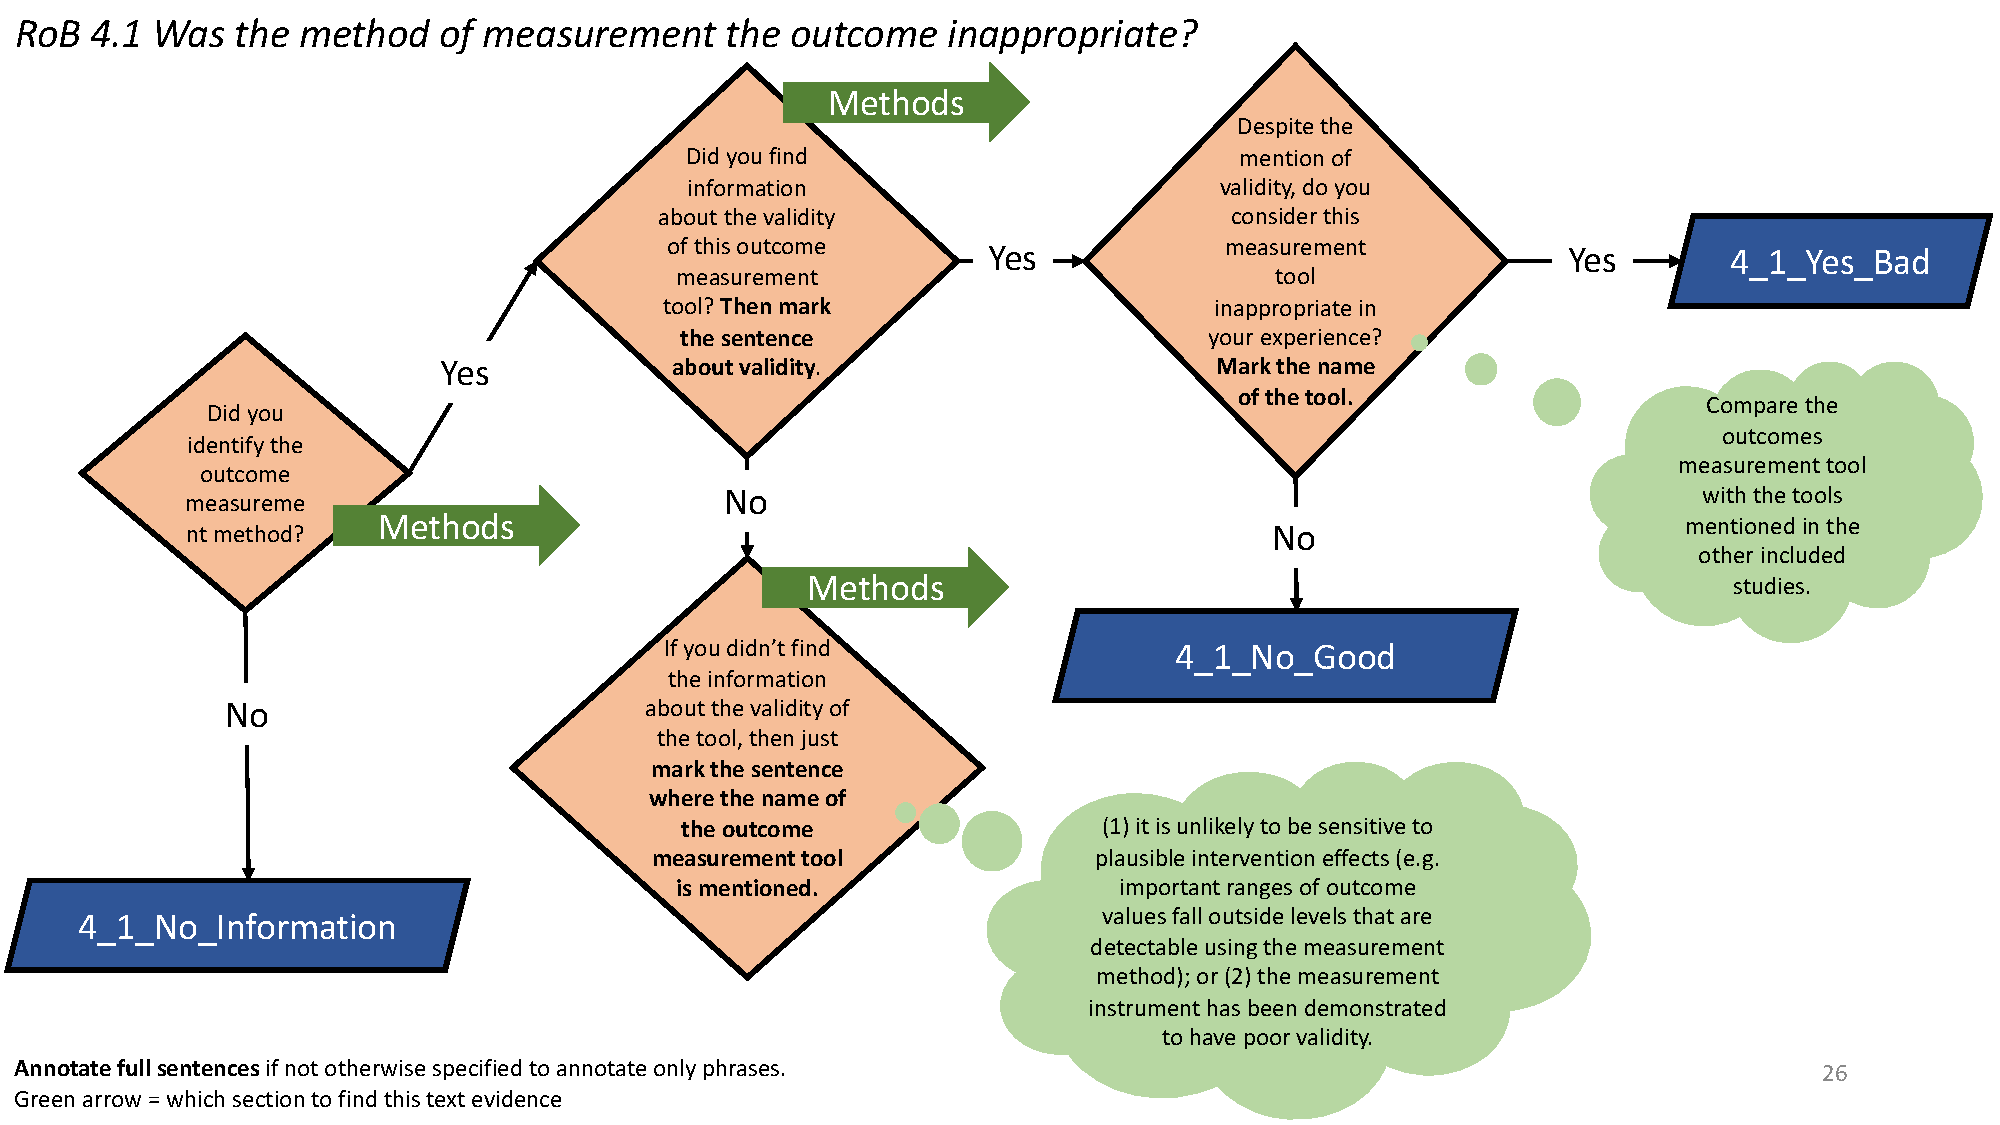
\includegraphics[width=\textwidth]{figures/4_1.pdf}
    \caption{Annotation instructions for the RoB 4.1 signalling question.}
    \label{fig:4_1}
\end{figure}
%
%
%


For annotation instructions for this signalling question, ``RoB 4.1 Was the method of outcome measurement inappropriate?'' follow the Flowchart~\ref{fig:4_1}.
As per the explanation above, the flowchart requests the annotators to identify the measurement method for the outcome of interest.
If you find information about the validity of the measurement method, mark the sentences that discuss this along with the name of the measurement tool.
Despite the validity being clarified, assess whether you consider this outcome measurement as appropriate and label the marked sentences as ``4.1 Yes Bad'' if you believe the method was inappropriate or as ``4.1 No Good'' if you believe it was appropriate.
If there is no information about the validity of the measurement tool/method, mark the name of the outcome measurement and label it as ``4.1 No Information''.
This information is found in the Methods section of the RCTs.
%
%
%
\subsection*{Signalling question - 4.2 }
\label{subsec:4_2}
%
The signalling question 4.1 ``Could measurement or ascertainment of the outcome have differed between intervention groups?'' assesses whether outcome measurement methods could have differed between the intervention groups in a study.
This question examines whether the methods used for outcome measurement were valid, consistent and applied equally to all intervention groups.
For example, if one group is assessed using a more sensitive or specific measurement tool, it may lead to overestimation or underestimation of treatment effects compared to the other group leading to systematic biases.
In general, unequal or inconsistent outcome measurement methods between the groups can undermine the internal validity of the study~\cite{enwald2010preventing}. % Nevertheless, the effect of possible biases, such as relying solely on self-reports and on intervention design without a no-information control group, should not be underestimated.

%
%
%
\begin{figure}[hbt]
    \centering
    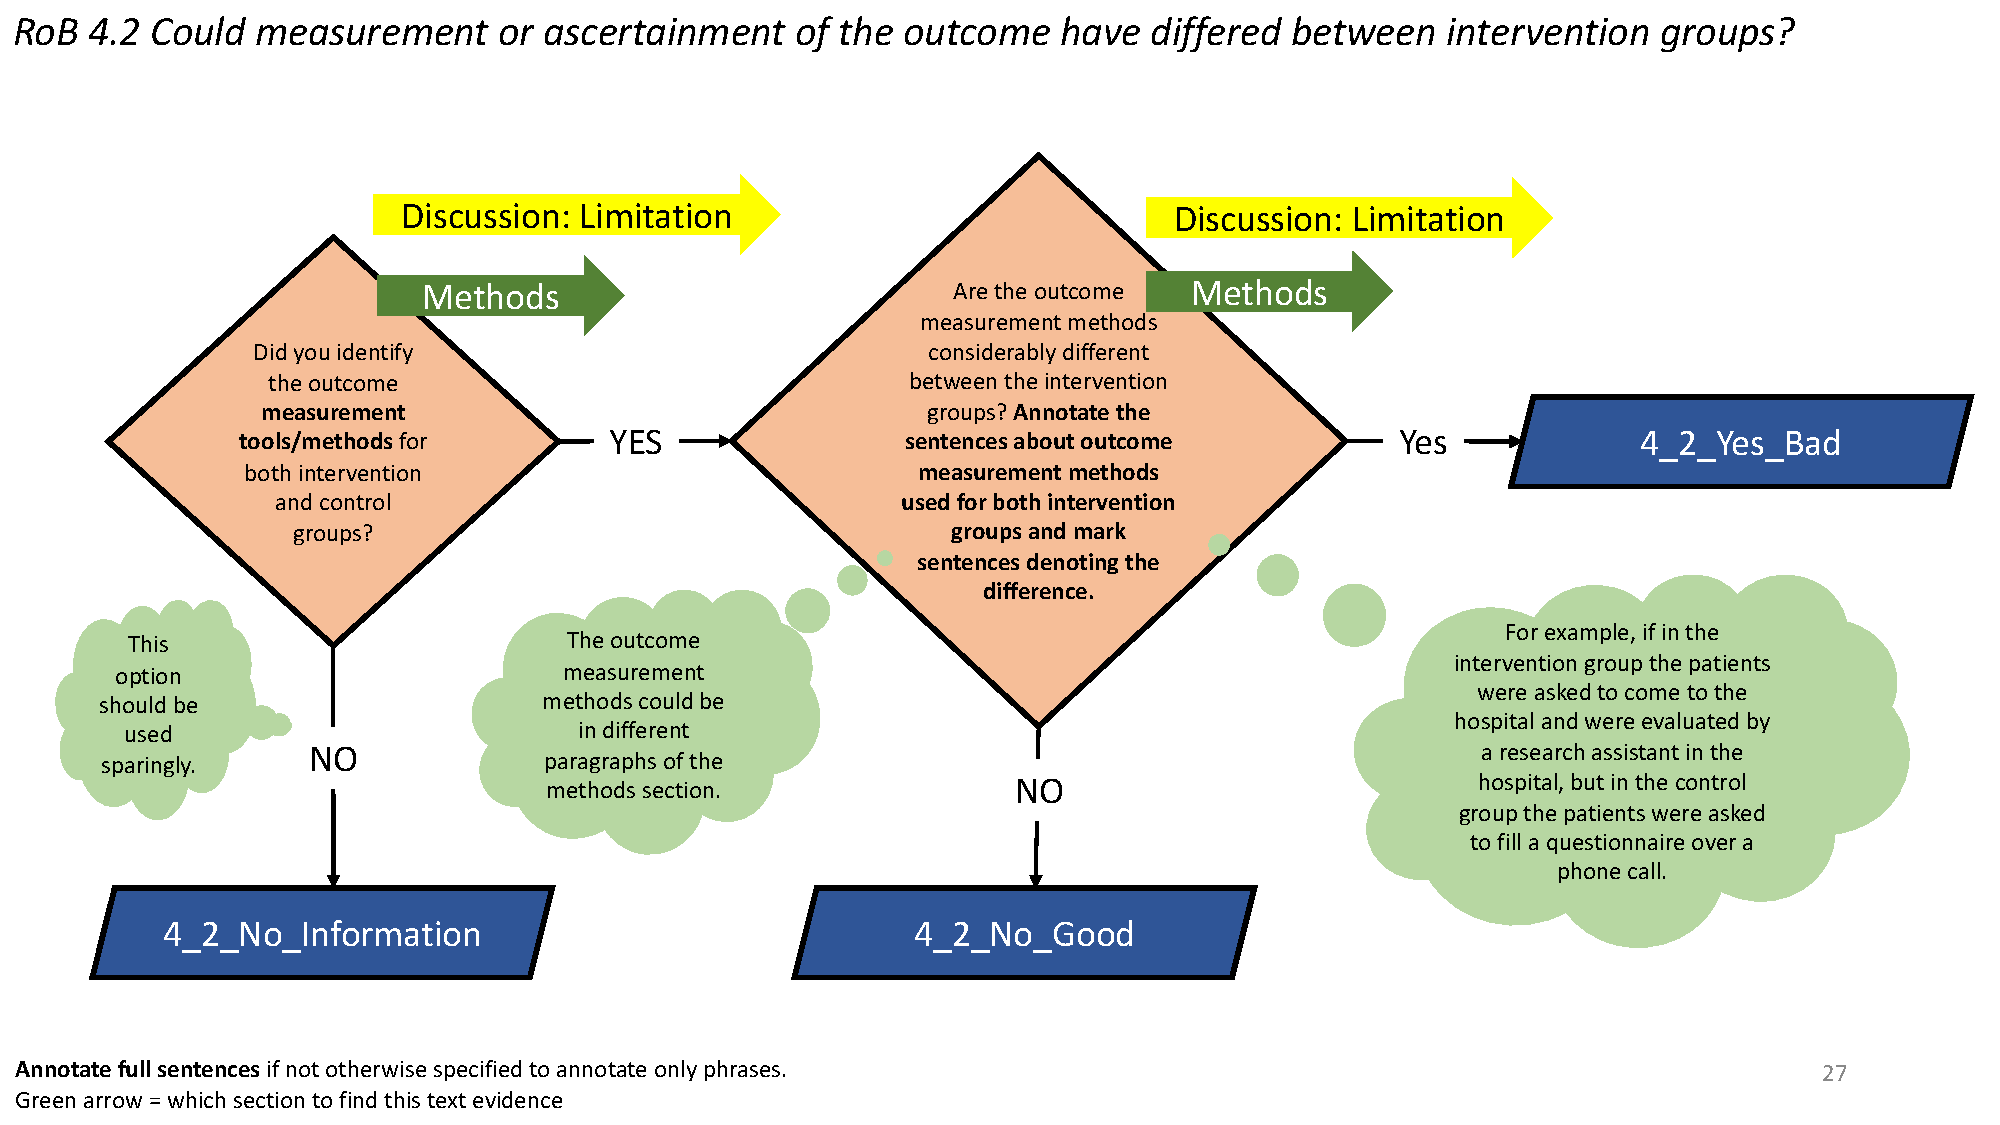
\includegraphics[width=\textwidth]{figures/4_2.pdf}
    \caption{Annotation instructions for the RoB 4.2 signalling question.}
    \label{fig:4_2}
\end{figure}
%
%
%

For annotation instructions for this signalling question, ``RoB 4.2 Could measurement or ascertainment of the outcome have differed between intervention groups?'' follow the Flowchart~\ref{fig:4_2}.
Following the explanation above, the annotators are asked to find the outcome measurement methods for all intervention groups (or intervention and control).
Mark the sentences describing outcome measurement methods from all intervention groups.
If the annotator identifies disparity between the outcome measurement methods, then label the sentences with ``4.2 Yes Bad'', and ``4.2 No Good'' otherwise.
For example, ``The control group's gait speed was measured using a standard stopwatch-based manual timing method. The intervention group's gait speed was measured using an advanced motion capture system.
This significant differences in measurement methods raises concerns regarding potential biases and systematic differences in outcome assessment.
In contrast, ``Both the control group and the experimental group utilized a validated visual analog scale (VAS) to assess pain intensity.''
The uniformity in the measurement methods increases the internal validity as well as comparability of the outcomes.
%
%
%
\subsection*{Signalling question - 4.3 }
\label{subsec:4_3}
%
The signalling question 4.3 ``Were outcome assessors aware of the intervention received by the study participants?'' assesses the blinding or masking of outcome assessors in a study.
If the outcome assessors are unblinded, they may unintentionally or inadvertently favour one one intervention over another based on preconceived notions about the interventions.
Blinding of outcome assessors is particularly important in studies where subjective outcomes are assessed which is the case in physiotherapy and rehabilitation.
For instance, a systematic review and meta-analysis on acupuncture for the treatment of peripheral neuropathy highlighted the potential bias introduced if outcome assessors are not blinded to treatment assignment~\cite{dimitrova2017acupuncture}.
Therefore, blinding the outcome assessors helps minimize the risk of bias and ensures that the assessments are conducted objectively and independently from knowledge of the intervention.
%- Inadvertently favor one intervention over another
%- Systematic differences in the outcome measurement (reduces accuracy and comparability)
%- recording outcomes in a way that aligns with their expectations.
%s- observer expectancy effect
%
%
%
\begin{figure}[hbt]
    \centering
    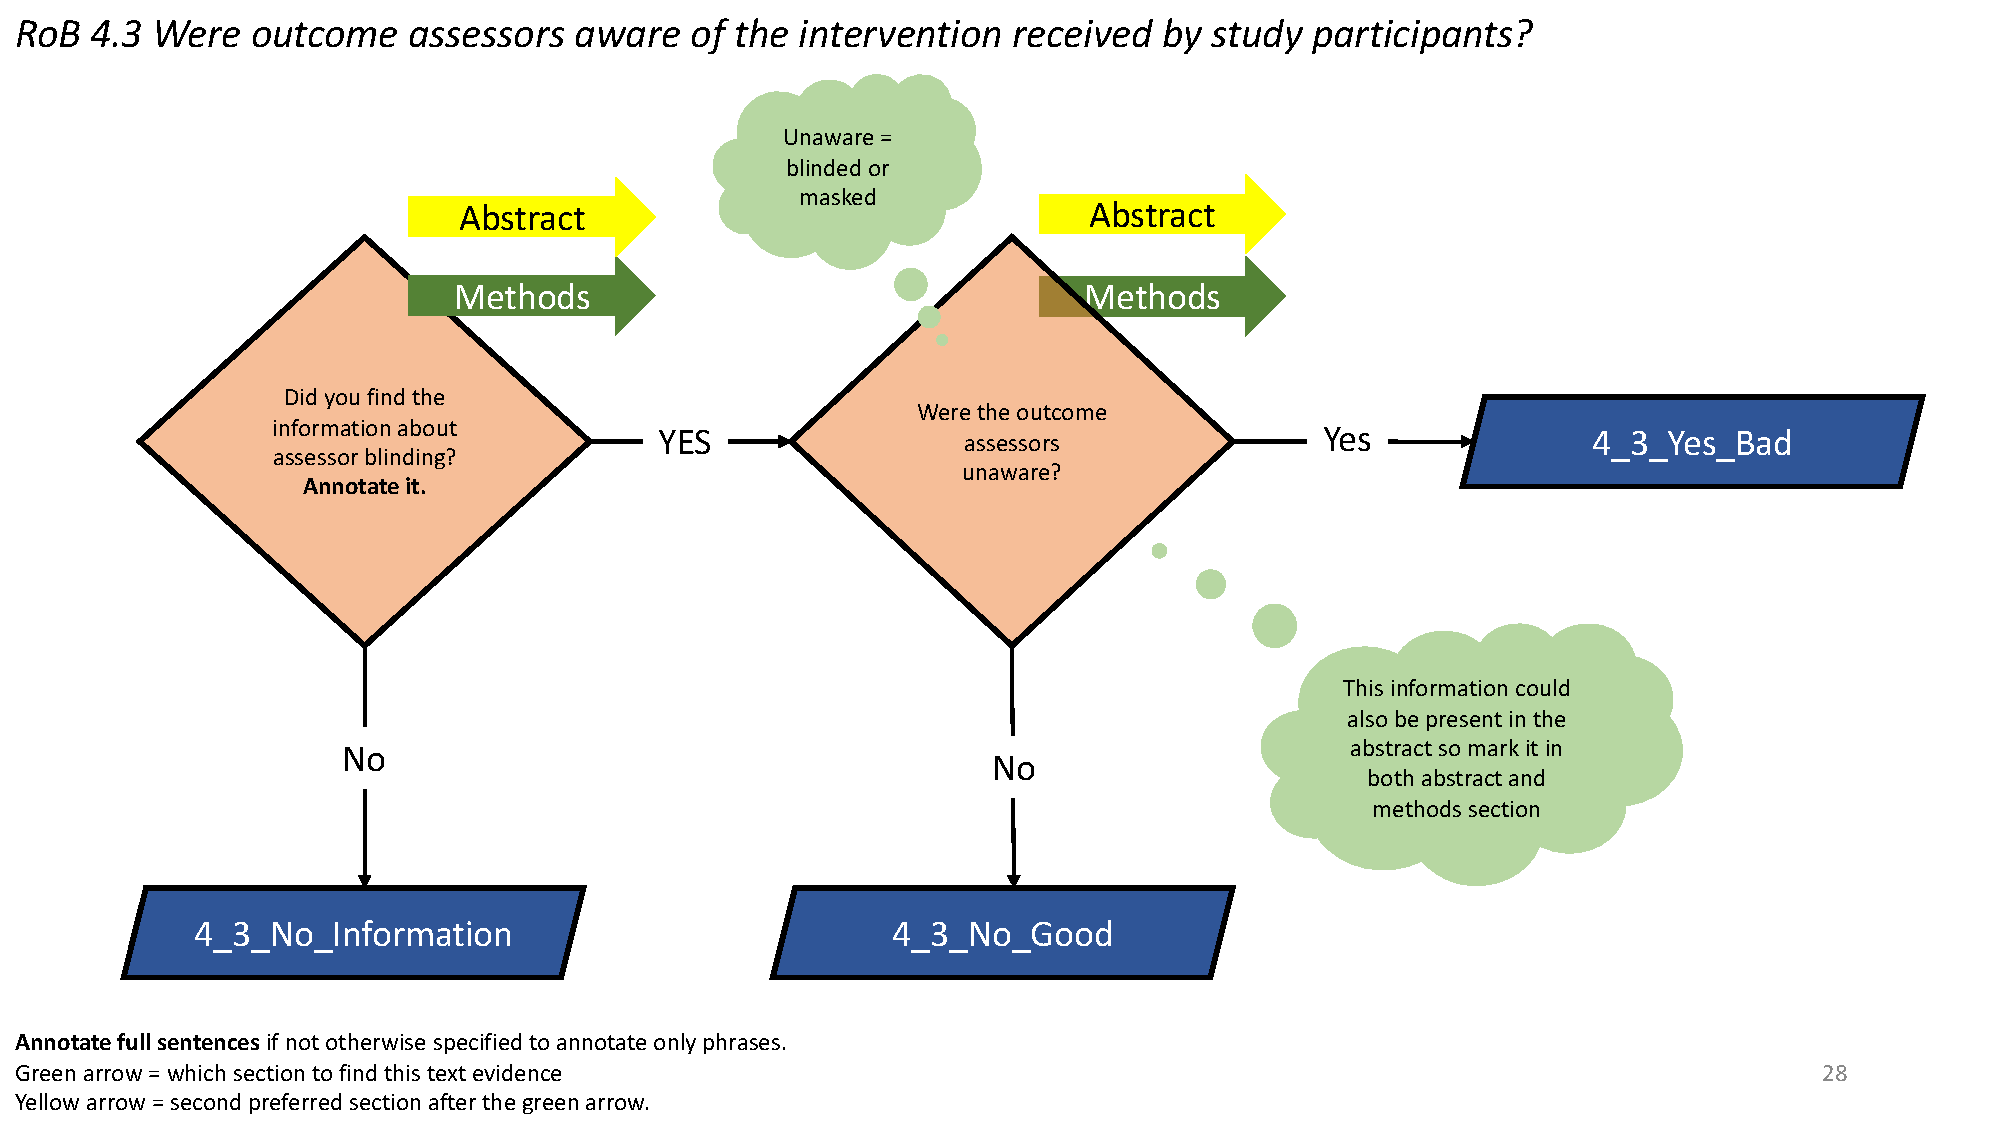
\includegraphics[width=\textwidth]{figures/4_3.pdf}
    \caption{Annotation instructions for the RoB 4.3 signalling question.}
    \label{fig:4_3}
\end{figure}
%
%
%


For annotation instructions for this signalling question, ``RoB 4.3 Were outcome assessors aware of the intervention received by the study participants?'' follow the Flowchart~\ref{fig:4_3}.
Following the explanation above, the first diamond in the flowchart instructs the annotators to identify information about assessor blinding. 
If assessor blinding information is not found, it will be automatically marked as ``2.3 No Information'' for this signalling question, following the  ``No'' arrow.
If proper assessor blinding description is found or the sentences describing that the outcome assessors were unaware of the assigned intervention, then annotate it and mark the sentence with ``4.3 No Good'' label.
In certain cases, outcome assessors are not blinded or could not be blinded, then mark such descriptions with label ``4.3 Yes Bad''.
For example, ``The outcome assessors were aware of the intervention received by participants, as the study aimed to evaluate the impact of a behavioral intervention on self-reported anxiety levels.''
This information if not found from the Methods sections, could also be annotated in the study abstract.

%
%
%
\subsection*{Signalling question - 4.4 }
\label{subsec:4_4}
%
The signalling question 4.4 ``Could assessment of the outcome have been influenced by knowledge of intervention received?'' evaluates the potential for bias resulting from outcome assessors' awareness of the intervention received by the participants.
This question aims to assess whether outcome assessments ``could'' have been influenced or biased by the assessors' knowledge of the intervention assignment.
As explained in the signalling question 4.3, that assessors awareness of assigned intervention could cause biases.

%
%
%
\begin{figure}[hbt]
    \centering
    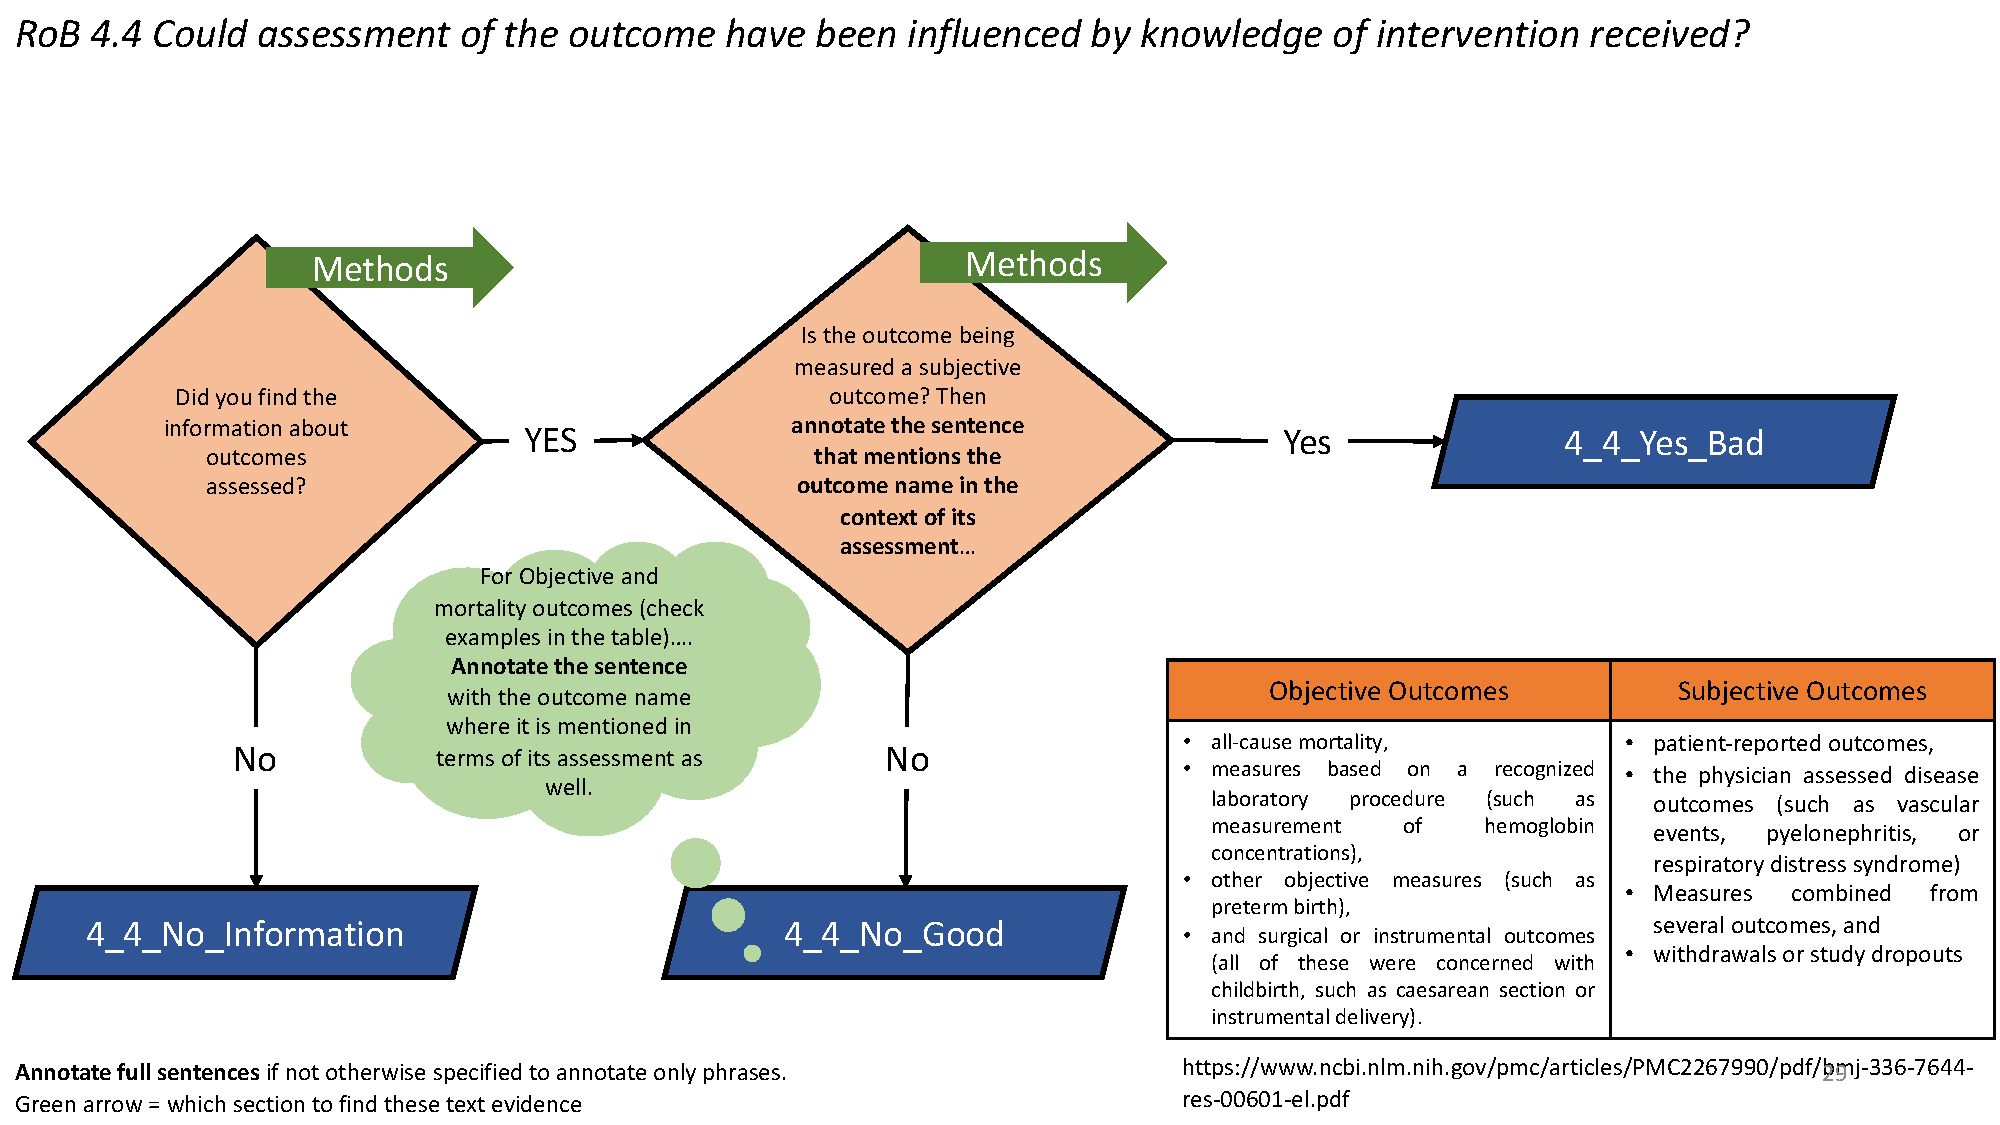
\includegraphics[width=\textwidth]{figures/4_4.pdf}
    \caption{Annotation instructions for the RoB 4.4 signalling question.}
    \label{fig:4_4}
\end{figure}



For annotation instructions for this signalling question, ``RoB 4.4 Could assessment of the outcome have been influenced by knowledge of intervention received?'' follow the Flowchart~\ref{fig:4_4}.
The first diamond in the flowchart asks the annotators to look for descriptions of outcomes assessed.
If the outcome of interest is subjective outcome, then annotate the sentence describing the outcome measurement in context of its assessment and label the description as ``4.4 Yes Bad''.
If the outcome of interest is objective outcome or mortality outcome, then annotate the sentence describing the outcome measurement in context of its assessment, but this time around label the description as ``4.4 No Good''.
For the domains of physiotherapy and rehabilitation, the question is quite theoretical and solely depends on whether the outcome assessed was subjective, objective or mortality.


%
%
%
\subsection*{Signalling question - 4.5 }
\label{subsec:4_5}
%
The signalling question 4.5 ``Is it likely that the assessment of the outcome was influenced by knowledge of the intervention received?'' evaluates the likelihood that the outcome assessment was biased due to assessors' knowledge of the intervention received by the participants.
The question is similar to the question 4.4, but it directly asks about the likelihood of the assessment being influenced by knowledge of the intervention.
It seeks a determination of the probability or likelihood of such an influence being present.


%
%
%
\begin{figure}[htbp]
    \centering
    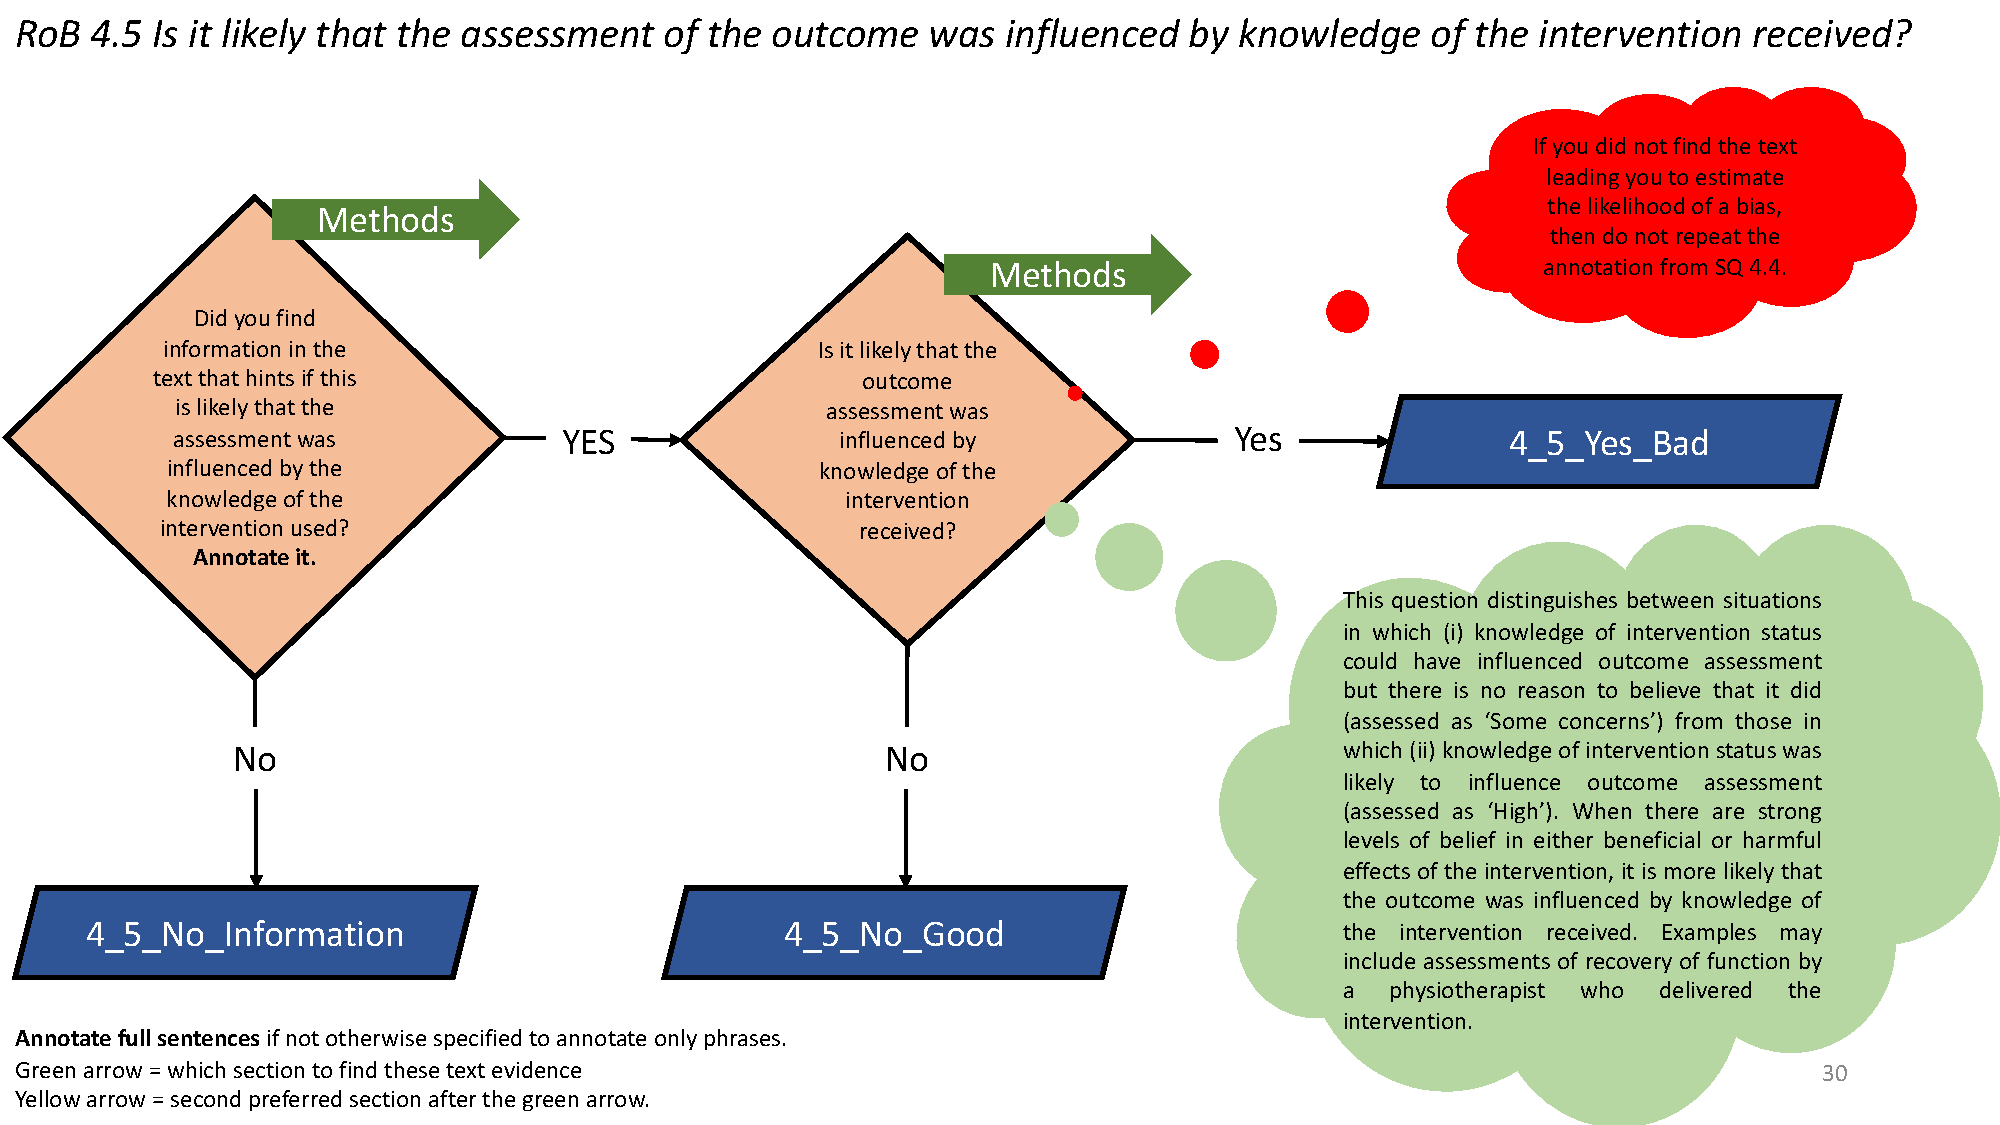
\includegraphics[width=\textwidth]{figures/4_5.pdf}
    \caption{Annotation instructions for the RoB 4.5 signalling question.}
    \label{fig:4_5}
\end{figure}
%
%
%


For annotation instructions for this signalling question, ``RoB 4.5 Is it likely that the assessment of the outcome was influenced by knowledge of the intervention received?'' follow the Flowchart~\ref{fig:4_5}.
The first diamond in the flowchart asks the annotators to find text that hints if the outcome assessment was influenced by the knowledge of intervention used.
If such a text is identified, then is it likely that the outcome assessment was influenced by the knowledge of the intervention received, if no the mark the identified description with the label ``4.5 No Good'', and otherwise as ``4.5 Yes Bad''.
The information is likely found in the Methods section.

%
%
%
%%%%%%%%%%%%%%%%%%%%%%%%%%%%%%%%%%%%%%%%%%%%%%%%%%%%%
\section*{Annotation Guidelines for RoB domain 5}
\label{sec:dom5}
%%%%%%%%%%%%%%%%%%%%%%%%%%%%%%%%%%%%%%%%%%%%%%%%%%%%%
%
Risk domain 5 in RoB 2 tool refers to the ``Bias in the selection of reported results'' domain.
This domain assesses the risk of bias that may arise from the selective reporting of outcomes or analyses within a study.
Selective reporting can lead to biased or incomplete reporting of results, which may distort the overall findings and affect the interpretation of the study's conclusions.
The assessment of risk domain 5 helps determine whether the study has adequately reported all the intended outcomes and analyses as specified in the study protocol or pre-specified plans.
This ensures transparency and reduces the risk of bias arising from selective reporting.
%
%
%
\subsection*{Signalling question - 5.1 }
\label{subsec:5_1}
%
The signalling question 5.1, ``Were the data that produced this result analyzed in accordance with a pre-specified analysis plan that was finalized before unblinded outcome data were available for analysis?'' evaluates whether particular results were analyzed according to a pre-defined analysis plan that was established before the researchers had access to the unblinded outcome data.
Suppose the analysis plan was established before accessing the unblinded outcome results and was followed correctly after obtaining the results; then it suggests that the analysis was conducted independently of the researcher's knowledge of the outcome, reducing the potential for bias in the interpretation of the data.
If an analysis plan was established until after accessing the results of the outcome, then some risk of bias could be introduced by knowledge of the results~\cite{riiser2022cycling}. % The randomized controlled trials included in the meta-analysis were considered to have a low risk of bias because they had a predefined analysis plan.
Assessment of this domain requires trial protocol document in addition to the trial itself.
In our work, one of the annotators manually retrieved and attached the pdf of trial protocol to the clinical trial study.
%
%
%
\begin{figure}[htbp]
    \centering
    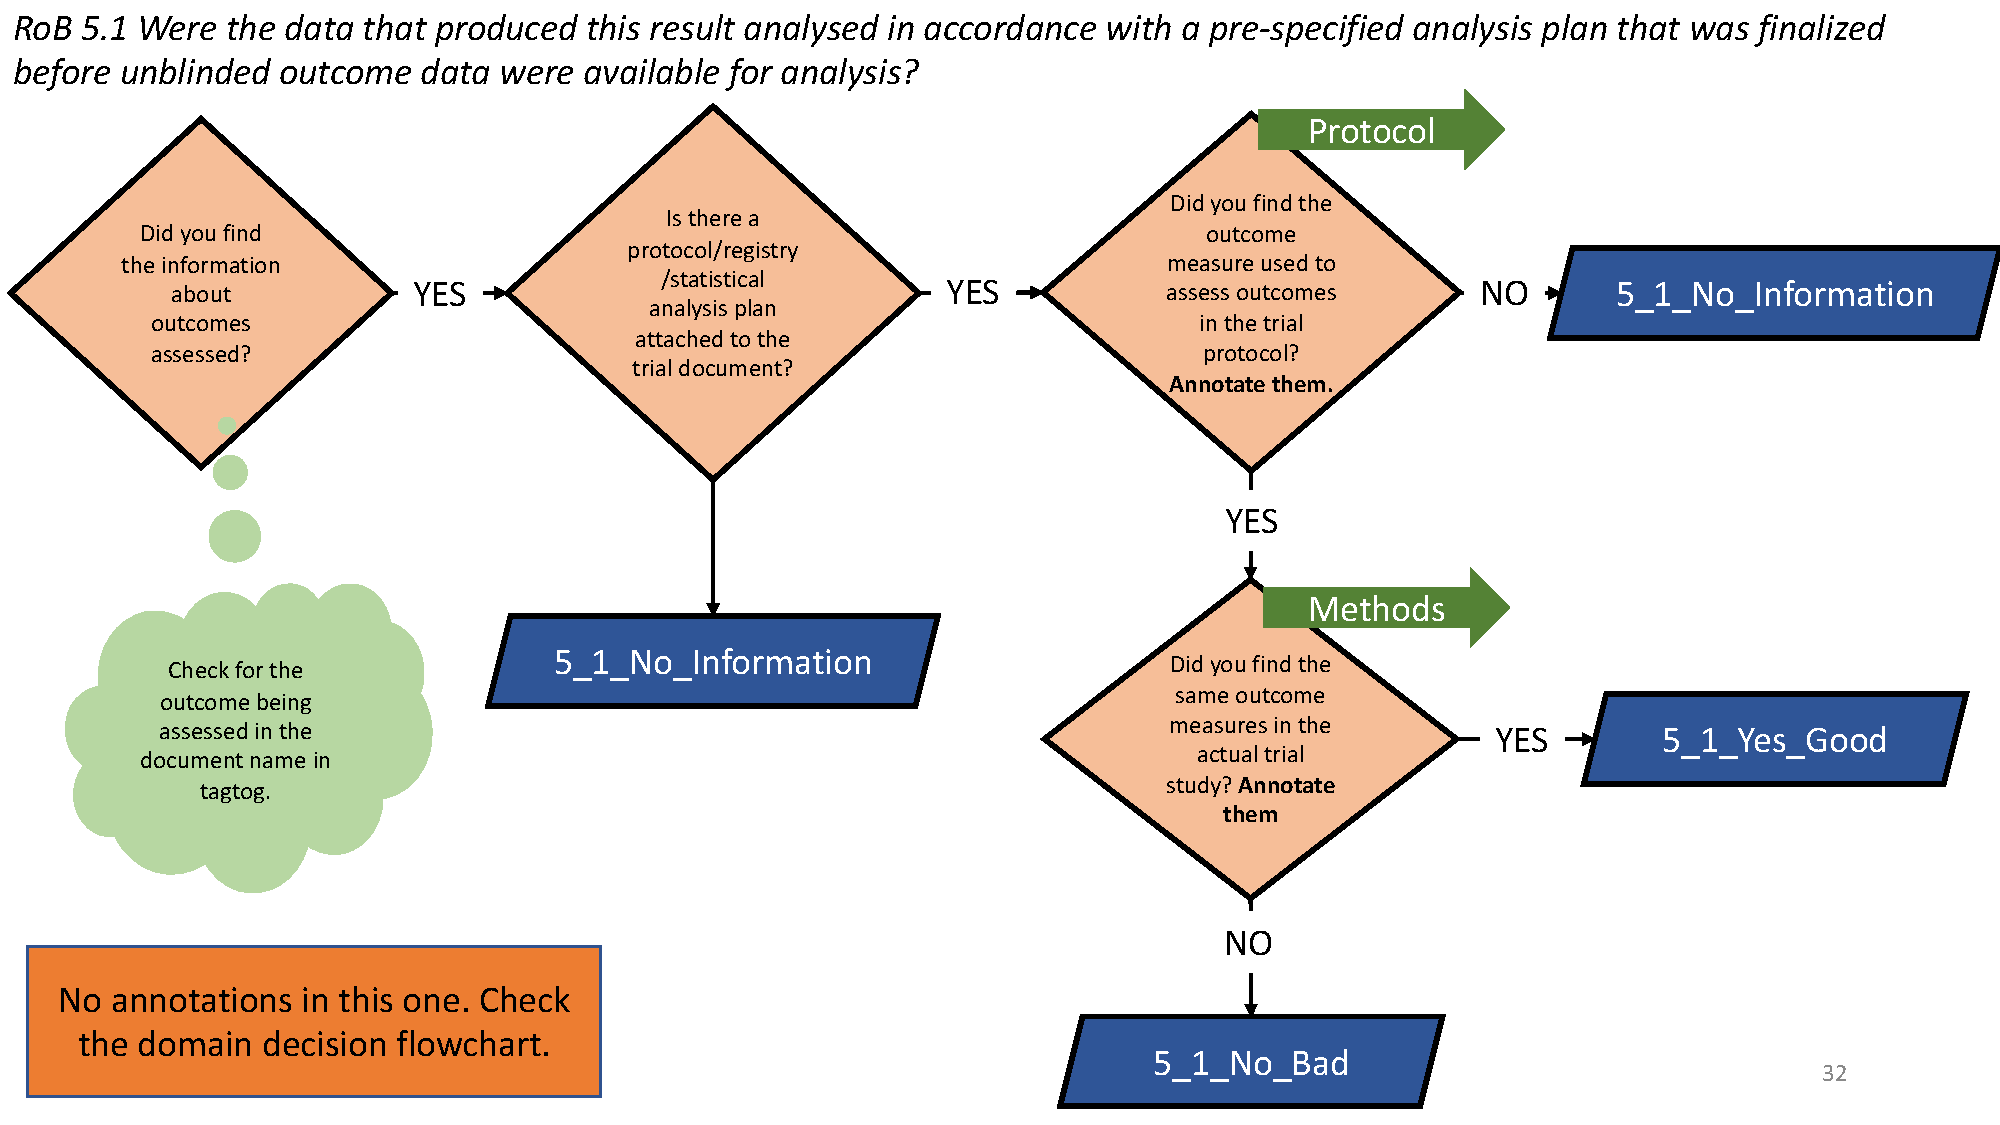
\includegraphics[width=\textwidth]{figures/5_1.pdf}
    \caption{Annotation instructions for the RoB 5.1 signalling question.}
    \label{fig:5_1}
\end{figure}
%
%
%

For annotation instructions for this signalling question, ``RoB 5.1 Were the data that produced this result analysed in accordance with a pre-specified analysis plan that was finalized before unblinded outcome data were available for analysis?'' follow the Flowchart~\ref{fig:5_1}.
In accordance with the explanation above, the first diamond in the flowchart asks the annotators to find the outcomes of interest that were assessed. 
Next, they are requested to check whether any protocol/registry/statistical analysis plan attached to the trial document.
If a trial protocol is not found, then the study will be automatically considered as ``5.1 No Information'' for this signalling question.
If a trial protocol is found, follow to identify the outcome measurements used to assess the outcome(s) of interest.
Annotate them
This information should be found in the trial protocol and if not found then the study will be automatically considered as ``5.1 No Information''.
Are the outcome measures in the clinical trial the same as outcome measures as listed in the trial protocol?
This information should be found in the methods section of the clinical trial.
Annotate the information. 
If the outcome measures as listed in the protocol and the clinical study are same, then label the trial as ``5.1 Yes Good'' and otherwise ``5.1 No Bad''.



%
%
%
\subsection*{Signalling question - 5.2 }
\label{subsec:5_2}
%
The signalling question 5.2, ``Is the numerical result being assessed likely to have been selected, on the basis of the results, from multiple eligible outcome measurements (e.g. scales, definitions, time points) within the outcome domain?'' aims to evaluate whether the researchers selectively chose a specific result among various possible outcome measurements, such as different scales, definitions, or time points, based on the findings they obtained.
If researchers have access to multiple outcome measurements and choose the one that yields a favourable or significant result, it can introduce bias and compromise the objectivity of the findings. 
Evaluating this risk of bias helps assess whether the reported result was genuinely chosen based on a predetermined protocol plan or selectively chosen based on the obtained results, potentially introducing a bias in favour of a particular outcome measurement.


%
%
%
\begin{figure}[htbp]
    \centering
    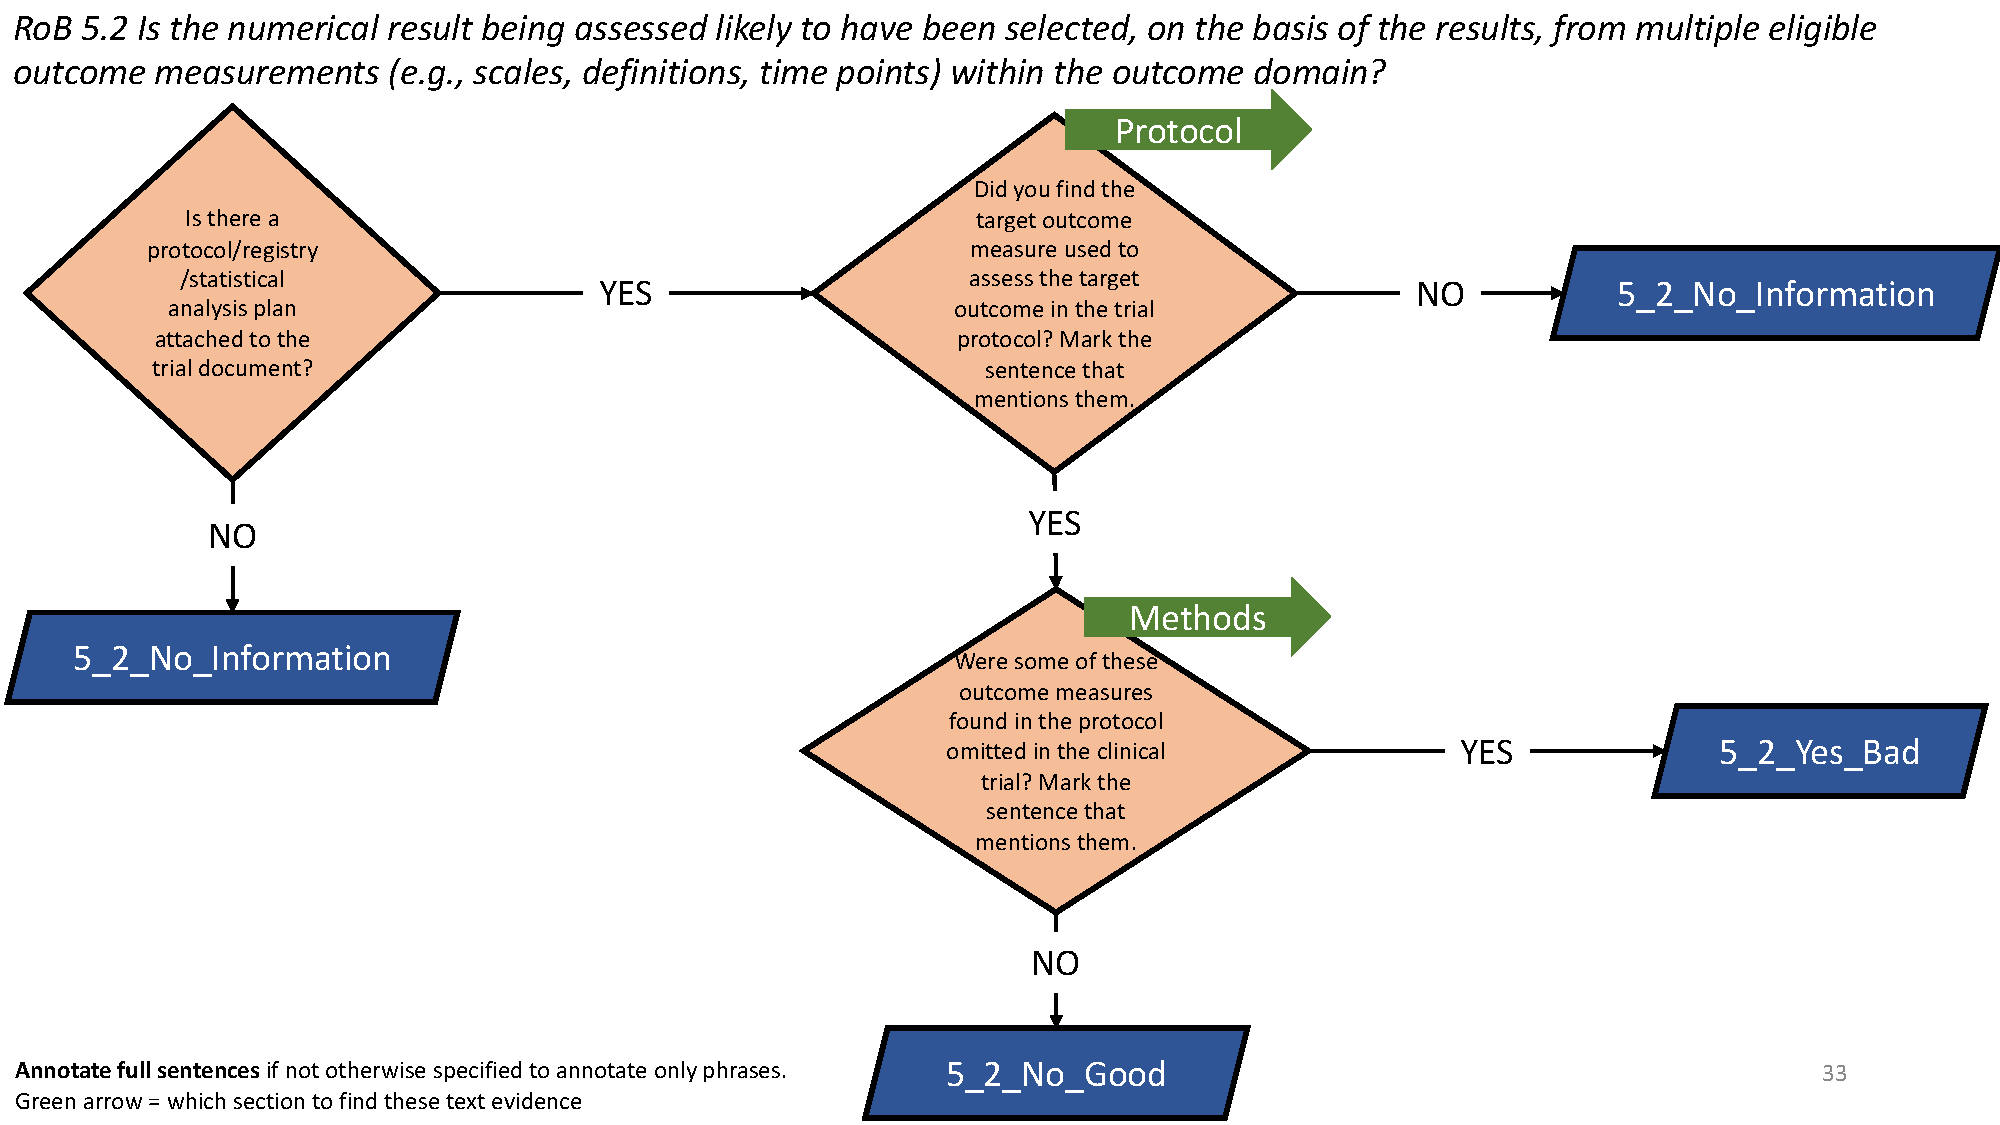
\includegraphics[width=\textwidth]{figures/5_2.pdf}
    \caption{Annotation instructions for the RoB 5.2 signalling question.}
    \label{fig:5_2}
\end{figure}
%
%
%

For annotation instructions for this signalling question, ``Is the numerical result being assessed likely to have been selected, on the basis of the results, from multiple eligible outcome measurements (e.g. scales, definitions, time points) within the outcome domain?'' follow the Flowchart~\ref{fig:5_2}.
In accordance with the explanation above, the first diamond in the flowchart asks the annotators to find the outcomes of interest that were assessed. 
Next, they are requested to check whether any protocol/registry/statistical analysis plan attached to the trial document.
If a trial protocol is not found, then the study will be automatically considered as ``5.2 No Information'' for this signalling question.
If a trial protocol is found, follow to identify all the outcome measures used to assess the target outcome in the trial protocol? 
Mark the sentence that mentions them.
This information should be found in the trial protocol and if not found then the study will be automatically considered as ``5.2 No Information''.
Were some of these outcome measures found in the protocol omitted in the clinical trial?
Mark the sentence that mentions them.
This information should be found in the methods section of the clinical trial.
If all the outcome measures as listed in the protocol are reported in the clinical study, then label the trial as ``5.2 Yes Good'' and otherwise ``5.2 No Bad''.

%
%
%
\subsection*{Signalling question - 5.3 }
\label{subsec:5_3}
%
This signalling question 5.3, ``Is the numerical result being assessed likely to have been selected, on the basis of the results, from multiple eligible analyses of the data?'' aims to determine whether the researchers selectively chose a specific numerical result among various possible data analyses based on the findings they obtained.
When researchers have flexibility in conducting multiple analyses on the same dataset and selecting and reporting the analysis that yields favourable results and supports some hypothesis, it could potentially introduce some risk of bias.
Hence this question aims to analyse whether a predefined analysis plan was in place in the trial protocol and whether it was genuinely followed for results analysis and reporting to ensure transparency and mitigate the risk of biased reporting.


%
%
%
\begin{figure}[htbp]
    \centering
    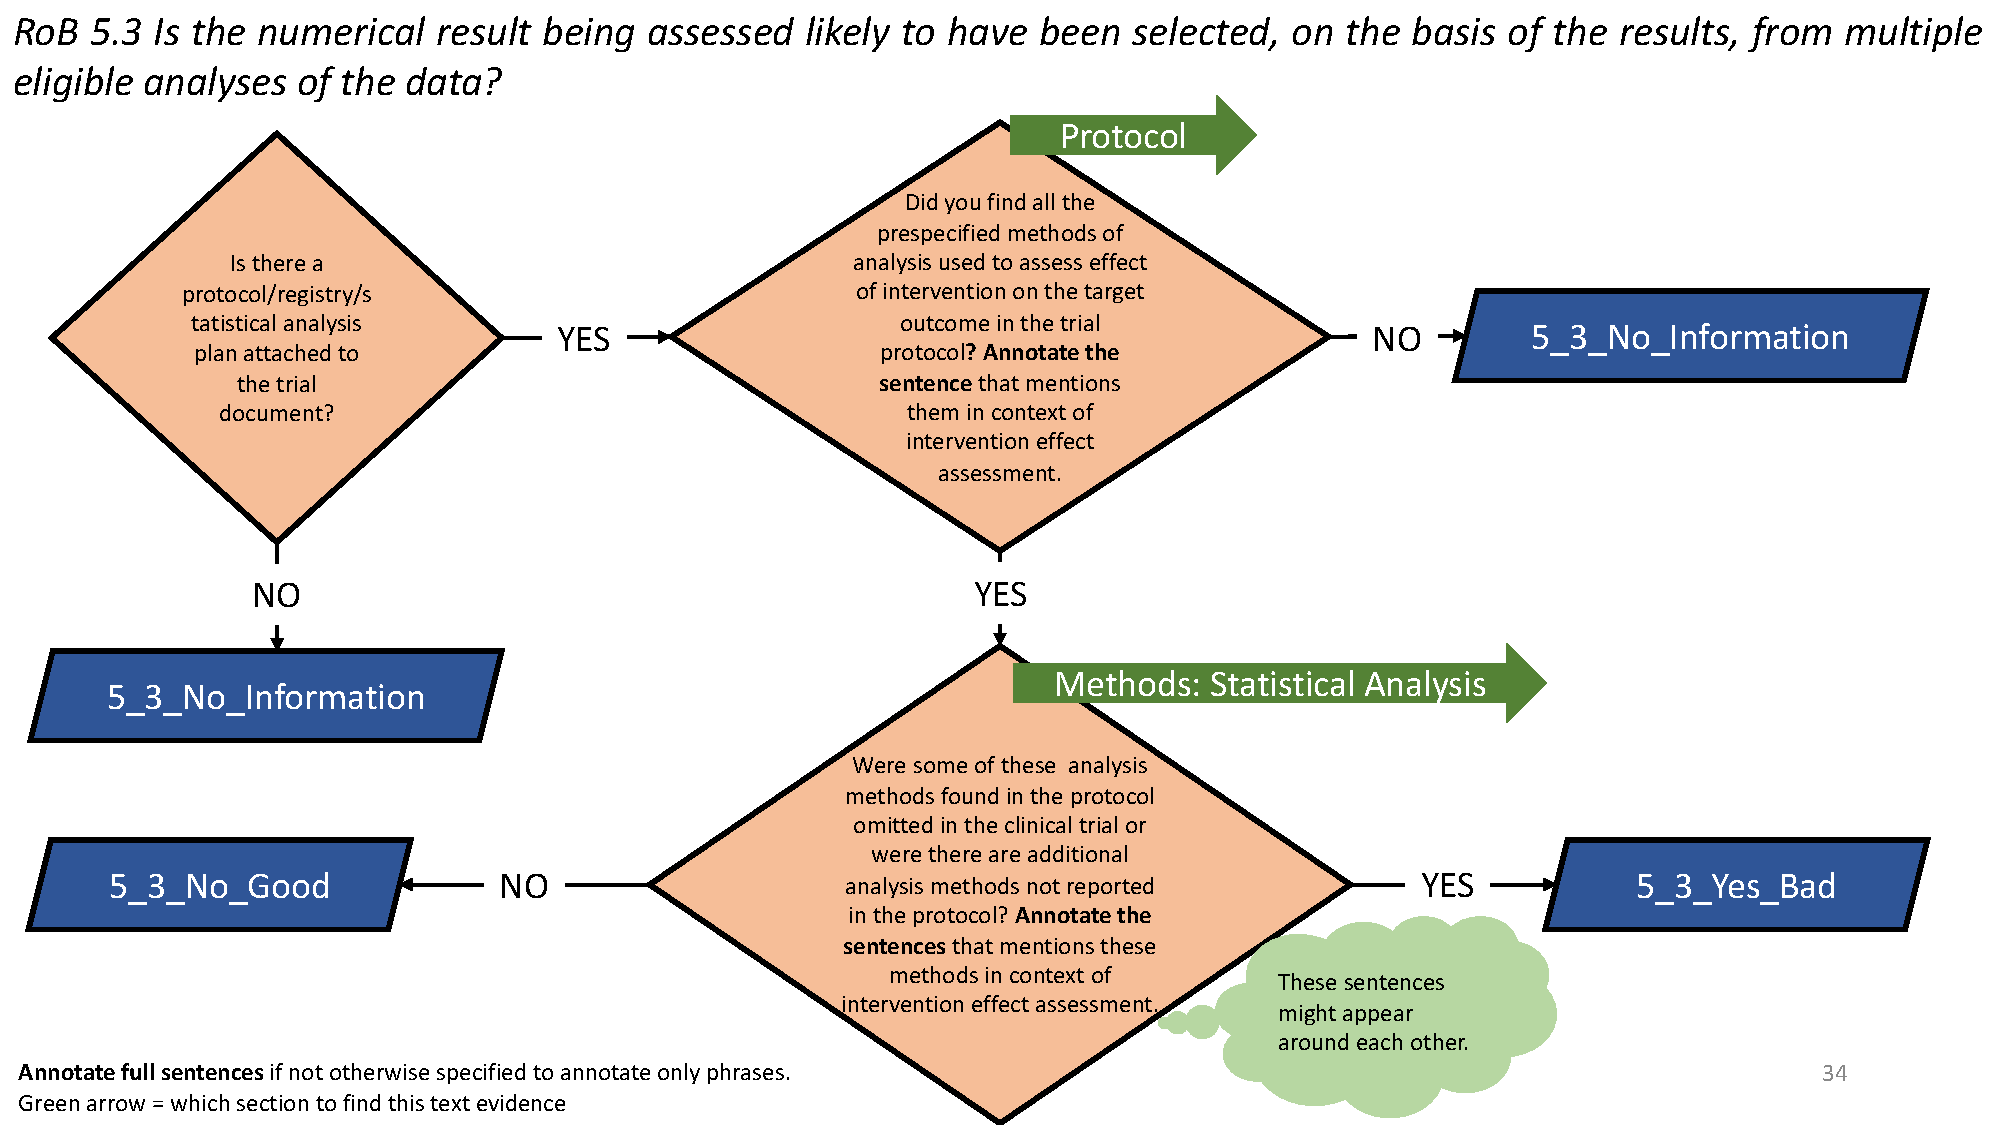
\includegraphics[width=\textwidth]{figures/5_3.pdf}
    \caption{Annotation instructions for the RoB 5.3 signalling question.}
    \label{fig:5_3}
\end{figure}
%
%
%

For annotation instructions for this signalling question, ``Is the numerical result being assessed likely to have been selected, on the basis of the results, from multiple eligible analyses of the data??'' follow the Flowchart~\ref{fig:5_3}.
In accordance with the explanation above, the first diamond in the flowchart asks the annotators if a trial protocol is found.
If a trial protocol is not found, then the study will be automatically considered as ``5.3 No Information''.
If a trial protocol is found, the annotators are asked to find all the prespecified methods of analysis used to assess effect of intervention on the target outcome in the trial protocol?
Mark the sentence that mentions them.
%This information should be found in the trial protocol and if not found then the study will be automatically considered as ``5.3 No Information''.
Check if all the outcomes analysis methods found in the trial protocol were also found in the clinical study.
If some of these  methods of analysis found in the protocol were omitted in the clinical trial or in case there are additional analysis methods not reported in the protocol, then annotate the sentence(s) that mentions these methods in context of intervention effect assessment.
If some of the methods were missing or some additional methods were conducted for outcomes analysis then label these descriptions as ``5.3 No Bad'' and otherwise ``5.3 Yes Good''.
This information should be found in the methods section (statistical analysis) of the clinical trial.
%
%
%
%%%%%%%%%%%%%%%%%%%%%%%%%%%%%%%%%%%%%%%%%%%%%%%%%%%%%
%\section*{Prompts for LLM evaluation}
%\label{sec:llms}
%%%%%%%%%%%%%%%%%%%%%%%%%%%%%%%%%%%%%%%%%%%%%%%%%%%%%
%
%The detailed results of LLM evaluation on 10 of the 60 RCTs are presented in this section.



%\textbf{Prompt: } Write your prompt here...
%\newline
%\textbf{Answer: } Write the answer that ChatPDF gave
%\newline
%\textbf{Discussion: } Individual discussion on the reply from ChatPDF
%
%
%
%\clearpage
%%===========================================================================================%%
%% If you are submitting to one of the Nature Portfolio journals using the eJP submission   %%
%% system, please include the references within the manuscript file itself. You may do this  %%
%% by copying the reference list from your .bbl file, paste it into the main manuscript .tex %%
%% file, and delete the associated \verb+\bibliography+ commands.                            %%
%%===========================================================================================%%
%\bibliographystyle{}
\bibliography{sn-bibliography.bib} % common bib file
%% if required, the content of the .bbl file can be included here once bbl is generated
%%\input sn-article.bbl


\end{document}